\documentclass[12pt,a4paper,twoside,openright]{report}
\usepackage{preamble} % imported packages/macros/styling from preamble.sty

\usepackage[sorting=none]{biblatex} % sorting=none means citations in bibliography appear in the order they are cited  
\usepackage[none]{hyphenat} % Disables hyphenation for the entire document. Words will no longer be split across multiple lines with hyphens
\addbibresource{ref.bib} % Add bibliography from ref.bib 

\begin{document}

% TC:ignore tells texcount to ignore word count until TC:endignore 

%TC:ignore

% ----------------------------------------------------------------------

% Title page 
\pagestyle{empty}

\rightline{\LARGE \textbf{Dylan Moss}}

\vspace*{30mm}
\begin{center}
	\Huge
	\textbf{Automatic Parallelisation using \\ Effect Tracking and Cost Analysis} \\[20mm]

	\vspace{-2mm}
	
\includegraphics[scale=0.5]{./figures/crest.png}
	\hspace{0mm}\\[20mm]
	\vspace{2mm}


	\LARGE
	Computer Science Tripos -- Part II \\[1mm]
	Queens' College \\[20mm]

	\Large
	\today
\end{center}

\newpage
\thispagestyle{empty}

% ----------------------------------------------------------------------

\pagestyle{plain}

\pagenumbering{roman}


% Declaration of originality
\section*{Declaration}

% Check the declaration of originality is up-to-date
I, Dylan Moss of Queens' College, being a candidate for Part II of the Computer Science Tripos, hereby declare that this dissertation and the work described in it are my own work, unaided except as may be specified below, and that the dissertation does not contain material that has already been used to any substantial extent for a comparable purpose. In preparation of this dissertation I did not use text from AI-assisted platforms generating natural language answers to user queries, including but not limited to ChatGPT. I am content for my dissertation to be made available to the students and staff of the University.

\emph{Signed:} Dylan Moss\\
\emph{Date:} \today

% Proforma
\chapter*{Proforma}
 {\large
  \begin{tabular}{ll}
	  Candidate number:   & 2432D                                        \\
	  Project Title:      & \bf Automatic Parallelisation using          \\ & \bf Effect Tracking and Cost Analysis \\
	  Examination:        & \bf Computer Science Tripos -- Part II, 2023 \\
	  Word Count:         & 11991\footnotemark[1]                        \\
	  Code Line Count:    & 6128\footnotemark[2]                         \\
	  Project Originator: & The Candidate and Prof. Alan Mycroft         \\
	  Project Supervisor: & Prof. Alan Mycroft                           \\
  \end{tabular}
 }
\footnotetext[1]{This word count was computed using {\texttt{texcount}}.}
\footnotetext[2]{This code line count was computed using {\texttt{cloc}} (excluding autogenerated test output).}
\stepcounter{footnote}

\section*{Original Aims of the Project}
The core aim was to implement automatic parallelisation into the compiler of a mid-featured, imperative programming language. This language, dubbed \textit{Kautuka}, implements a sensible subset of Go. The automatic parallelisation compiler translates Kautuka into parallelised Go, utilising \textit{side-effect tracking} and \textit{cost analysis} to produce \textit{safe} and \textit{efficient} parallel code. This eliminates the need for parallelisation primitives (which require complex mental models) to exploit the benefits of multicore parallelism. Kautuka's performance would be evaluated against sequential Go. Extensions include: implementing an inference algorithm, adding I/O operations (with aliasing analysis), and developing tools which integrate Kautuka into existing workflows.

\section*{Work Completed}

Exceeded all success criteria and the majority of extensions. Kautuka supports variables, control flow, functions, and user I/O operations. Kautuka produces parallelised code which outperforms sequential Go on I/O-bound programs (the target candidates for performance improvements). I extended side-effect tracking with aliasing analysis, to track file references in file-I/O operations. I implemented an inference algorithm into cost analysis, allowing me to translate of hundreds of lines of Go into Kautuka with minimal overhead. I demonstrated how Kautuka can be integrated into existing workflows, enabling its gradual adoption into established Go codebases.

\section*{Special Difficulties}

None.

% Table of contents 
\tableofcontents


% ----------------------------------------------------------------------
\newpage
\pagenumbering{arabic}
\setcounter{page}{1}
%TC:endignore

% textcount's word count is now enabled 


% Remove code snippets and algorithms from word count 
%TC:envir minted 1 xall 
%TC:macro \mintinline [ignore]
%TC:envir algorithmic 1 xall

% Include tables in word count
%TC:envir table 0 word
%TC:envir tabular 1 word

% Include footnotes in word count
%TC:macro \footnote [text]
%TC:macro \footnotetext [text]

% Word-count hacking... (not recommended)
%TC:macro \hyperref [ignore]
%TC:macro \ignore [ignore]
%TC:macro \path [ignore]


% Main chapters
\addtocontents{lol}{\protect\vspace*{10pt}}
\chapter{Introduction}
\label{sec:1}

Since the mid 2000s, single-core processor performance has stagnated, with performance gains primarily achieved through \textit{multicore parallelism}. Modern programming languages allow programmers to specify parallel execution behaviour (how code is executed across multiple cores) to improve program performance.

However, parallelisation is inherently non-deterministic, resulting in \textit{race conditions}: where a program's output depends on the interleaving order of its threads. Race conditions give rise to a new category of bugs known for their elusive nature, only manifesting in certain thread interleavings. Since many programming languages do not ensure correctness in parallel programs (that is the absence of race conditions), the onus is on the programmer to detect these bugs, which is both challenging and prone to error. In addition, executing programs across multiple cores necessitates inter-core communication: a costly operation which may result in worse performance compared to the original sequential program. Despite its potential for enhancing performance, multicore parallelism poses significant challenges when writing \textit{safe} and \textit{efficient} parallel programs. 

\textit{Automatic parallelisation compilers} alleviate these problems by automatically compiling sequential code into parallel code, ensuring the produced code is safe and efficient with minimal programming overhead. There are two main approaches to automatic multicore parallelisation. The first is \textit{data-level parallelisation}: running the same operation on multiple memory locations at once. This low-level approach is effective at parallelising loops and other vectorisation operations, and is often found in mainstream imperative programming language compilers. It is best suited at optimising data-intensive computations, where loops tend to make up most of the execution time~\cite{doi:10.1080/09720529.2021.1951435}. The alternative approach is \textit{task-based parallelisation}: parallelising groups of code representing an individual task. In this project, each code block is considered a task --- denoted by wrapping a group of code in a pair of isolated curly braces. This naturally extends the typical use of code blocks: grouping together statements which perform the same ``task'' into a new scope, as threads (parallelised code blocks) follow the same scoping rules as code blocks. The pseudocode below illustrates an example of task-based parallelisation.

\vspace{2mm}

\begin{tikzpicture}
  
  \node[] (image) at (0, 0) { 

  \noindent\begin{minipage}{.5\textwidth}
  \begin{minted}{python}
    {
      for i in range(1000) { 
        print(i)
      }
    }

    {
      x := 0 
      for j in range(1000) { 
        x += j
      }
    }
  \end{minted}
  \end{minipage}%
  \begin{minipage}{0.5\textwidth}
    \begin{minted}{python}
      new thread(){
        for i in range(1000) { 
          print(i)
        }
      }.run()

      new thread(){
        x := 0 
        for j in range(1000) { 
          x += j
        }
      }.run()
    \end{minted}
  \end{minipage}
};

\draw [-latex, ultra thick] (-1.8, 0) -- node[midway, above, align=center]{parallelise} (0.5, 0);

\end{tikzpicture}

\vspace{3mm}

\newpage 

Task-based automatic parallelisation, also known as \textit{high-level automatic parallelisation}, aims to improve the performance of programs containing large, independent tasks. Implementations in literature typically focus on toy functional languages as opposed to imperative languages, as this approach requires complex static analysis. However, despite the prevalence of imperative programming languages, the applications of high-level automatic parallelisation in such languages remains largely unexplored. 

Literature on high-level automatic parallelisation dates back to 1970s~\cite{10.1145/1478462.1478537} — describing how to perform parallelisation in the presence of effectful code~\cite{10.1145/73560.73564} and aliasing~\cite{10.1007/978-3-540-30579-8_14}. However, despite extensive research, the lack of practical implementations (which integrate into existing workflows) has led to slow adoption rates of this technology. This project aims to provide a practical implementation of high-level automatic parallelisation, while exploring its potential in imperative programming languages. 

\section{Project Summary}
\label{sec:1.1}

In this project, I designed a \textit{mid-featured, sequential, imperative programming language} with an \textit{accompanying high-level automatic parallelisation compiler}. My language (hereby dubbed \textit{Kautuka}, after the Indian ritual \textit{thread}) implements a sensible subset of Go with minor syntactic changes. The compiler automatically compiles (sequential) Kautuka to parallel Go code, which can be executed using Go's compiler.

I theorised that high-level automatic parallelisation could improve the performance of I/O-bound programs. This drove my decision to use Go as the compilation target, as it provides robust support for I/O operations and efficient parallelisation primitives. Since Kautuka compiles straight to Go, we can integrate Kautuka into existing Go codebases without disrupting existing workflows. However, much of this work is language agnostic, and generalises to other imperative programming languages beyond Go. 

High-level parallelisation in imperative languages introduces complexities not commonly found in toy functional languages (such as variable mutation, for-loops, and imperative-style functions). This project addresses both the theoretical and practical challenges presented by these issues.

The focus of this dissertation is on designing, implementing, and evaluating a software engineering project. However, I also decided to explore three research questions to help inform my requirements analysis (section \hyperref[sec:2.7]{2.7}) and form the basis of my evaluation (section \hyperref[sec:4]{4}):

\begin{itemize}
  \item \textit{Does high-level automatic-parallelisation theory, previously developed for toy functional languages, transfer across to a full-featured imperative language?} In sections \hyperref[sec:2.4]{2.4} to \hyperref[sec:2.6]{2.6}, I explain the theoretical extensions needed to make this transition, and in section \hyperref[sec:3.5]{3.5} I describe \textbf{a novel approach to cost analysis (execution time estimation) to overcome constraints found in imperative languages.}
  \item \textit{Can I/O-bound programs benefit from high-level automatic parallelisation?} In section \hyperref[sec:2.4]{2.4}, I design the theory required for I/O parallelisation. Section \hyperref[sec:4.3]{4.3} demonstrates that \textbf{Kautuka's performance exceeds that of equivalent sequential Go code for I/O-bound programs}. 
  \item \textit{Are there real-world applications of this compiler?} In section \hyperref[sec:3.5]{3.5}, I implement a powerful cost-inference algorithm to minimise user annotations. This improves the accessibility of this language to the average programmer. In section \hyperref[sec:4.4]{4.4} I demonstrate how \textbf{Kautuka can be integrated into existing Go codebases with minimal effort.}
\end{itemize}


\addtocontents{lol}{\protect\vspace*{10pt}}
\chapter{Preparation}
%TC:envir minted 1 xall 
%TC:envir algorithmic 1 xall

% Include tables in word count
%TC:envir table 0 word
%TC:envir tabular 1 word

% Include footnotes in word count
%TC:macro \footnote [text]
%TC:macro \footnotetext [text]

%TC:group minted 0 0
%TC:macro \mintinline [ignore]
%TC:macro \colb [ignore]

%TC:macro \ignore [ignore] 
%TC:macro \hyperref [ignore]

\label{sec:2}

\newcommand{\ignore}[1]{#1}
\newcommand{\bound}[2]{\langle{#1, #2}\rangle}

High-level automatic parallelisation utilises \textit{effect systems} to produce \textit{safe} and \textit{efficient} parallel code. Parallel code is \textit{safe} if it avoids race conditions (such as the concurrent execution of \ignore{\mintinline{go}{x = 1}} and \ignore{\mintinline{go}{x = 2}}), and \textit{efficient} if it outperforms the original sequential code. Effect systems augment classical type systems with \textit{effects}, to reason about program execution behaviours such as side effects and execution time. Similar to type systems, effect systems consist of \textit{typing judgements} which infer expression properties --- the execution time of \ignore{\mintinline{go}{e1;e2}} can be inferred to be the sum of \ignore{\mintinline{go}{e1}} and \ignore{\mintinline{go}{e2}}'s execution times.

In sections \hyperref[sec:2.4]{2.4} to \hyperref[sec:2.6]{2.6}, I outline three effect systems required for my implementation of automatic parallelisation. \textit{Side-effect systems} (section \hyperref[sec:2.4]{2.4}) prove that parallelisation is safe while \textit{type-cost} (section \hyperref[sec:2.5]{2.5}) and \textit{runtime-cost systems} (section \hyperref[sec:2.6]{2.6}) ensure that produced parallel code is efficient. These systems form the basis of my compiler implementation (sections \hyperref[sec:3.4]{3.4} and \hyperref[sec:3.5]{3.5}). Section \hyperref[sec:2.7]{2.7} details the project requirements and the software development practices followed throughout the project.

\section{Project Overview}

\label{sec:2.1}

The project consists of two components: the Kautuka language and the high-level automatic parallelisation compiler (hereby referred to as just \textit{the compiler}). This section describes the compilation process of Kautuka, and how Kautuaka can be integrated into existing Go codebases (section \hyperref[sec:2.1.1]{2.1.1}). Section \hyperref[sec:2.1.2]{2.1.2} outlines Kautuka's key language features, and section \hyperref[sec:2.1.3]{2.1.3} describes each step of the compilation process (and the purpose of each effect system).

\subsection{Compilation of Kautuka}

\label{sec:2.1.1}

\noindent\begin{minipage}{.5\linewidth}

  Kautuka's compiler is written in OCaml (ML); compiling Kautuka (Kau) into parallelised Go code. The produced Go code is then compiled into executable machine code using Go's existing compiler. The components implemented in this project are highlighted in grey on the tombstone diagram (fig. \hyperref[fig:tombstone]{2.1}).

\end{minipage}%
\hspace{1.5mm}\begin{minipage}{.5\linewidth}
  \hspace{3mm}
  \begin{tikzpicture}
    \begin{tombstonediagram}
      \compiler{cmp}{Kau}{Go}{ML}{}
      \program[anchor=prg-2-2.north east]{prg}{Program}{Kau}{at (cmp-1-1.north west)}
      \compiler{cmp2}{Go}{x86}{Go}{at (cmp-1-3.north east)}
      \program{prgo}{Program}{x86}{at (cmp2-1-3.north east)}
      \machine{mac}{ML}{at (cmp-2-2.south west)}
      \machine{mac}{Go}{at (cmp2-2-2.south west)}
      \machine{mac}{x86}{at (prgo-2-2.south west)}
      \highlightprogram{prg}
      \highlightcompiler{cmp}
    \end{tombstonediagram}
  \end{tikzpicture}
  \vspace{-3mm}
  \captionof{figure}{Kautuka Compilation}
  \label{fig:tombstone}
\end{minipage}

\vspace{2mm}

To integrate Kautuka into existing Go codebases, we expect the programmer to identify (sequential) Go files containing large, independent computations. These files can be translated into Kautuka by hand, as the languages share similar syntax. The programmer marks groups of code representing a single \textit{task} with curly braces (which we refer to as \textit{code blocks}). Our compiler then compiles Kautuka programs back to parallelised Go code, placing them alongside the Kautuka files. The Go codebase now contains parallelised Go files, and can be executed as normal using the standard Go compiler.

\subsection{Kautuka Language}

\label{sec:2.1.2}

Kautuka implements a sensible subset of Go (with minor syntactic changes), and closely resembles other C-like languages. This section provides a brief overview of all key language features.

Kautuka has the following types:

\vspace{-2mm}

\[ \tau ::= \textit{int, bool, string, unit, file\_ref, } \tau_1 * \cdots * \tau_n \rightarrow \tau \]

\vspace{-3mm}

where \( \tau_1 * \cdots * \tau_n \rightarrow \tau \) is the imperative-style function signature. Kautuka does not support currying or higher-order functions. Although I planned to implement recursion as a stretch goal, I was unable to complete this extension due to time constraints.

Kautuka does not support exponentiation, division, or modulus operations. Extending the language and compiler with division and modulus is relatively straightforward, however the exponentiation operator would be limited to only integer exponents\footnote{A decision explained in appendix \hyperref[sec:C]{C}.}. Kautuka includes a subtraction operator, but does not support negative numbers --- the responsibility is on the programmer to ensure that the result of subtraction is non-negative.

The language contains inbuilt console I/O functions: \textit{input} and \textit{print}, and file-I/O functions: \textit{open}, \textit{read}, \textit{write}, and \textit{append}. File references (of type \textit{file\_ref}) are obtained by calling the \textit{open} function with a filename string, and can be used to read and write to files. Disjoint file references are tracked using basic aliasing analysis (section \hyperref[sec:3.4]{3.4}), this project restricts aliasing analysis to just file references.

Kautuka also contains variables, control flow, functions, and code blocks (also referred to as just \textit{blocks}). Variables are declared with \ignore{\mintinline{go}{x := e}} and are assigned to with \ignore{\mintinline{go}{x = e}}. Variables declared in a local scope are bound to that scope. In Kautuka, variable types are inferred and so do not need to be annotated. \textit{For-loops} always take the form \ignore{\mintinline{go}{for x := e1; x < e2; x++ { e3 }}}, so that the number of loop iterations can be consistently estimated during cost analysis (section \hyperref[sec:3.5]{3.5}). Kautuka also supports for-each statements \ignore{\mintinline{go}{for x := range str { e }}}, iterating over every character of the string \ignore{\mintinline{go}{str}}. Functions are defined with \ignore{\mintinline{go}{func f(param_1 t_1, ..., param_n t_n) t { e }}}, where \ignore{\mintinline{go}{t}} is the function's return type and \ignore{\mintinline{go}{e}} contains at least one \ignore{\mintinline{go}{return}} statement (if the return type is \textit{non-unit}). Kautuka contains expressions (e.g., \ignore{\mintinline{go}{1 + 2}}), commands (e.g., \ignore{\mintinline{go}{x := 1}}), and structures (e.g., \ignore{\mintinline{go}{if true { 1 } else { 2 }}}). However, we treat commands and structures as unit-type \textit{expressions} to simplify our typing rules.

\subsection{Automatic Parallelisation Pipeline}

\label{sec:2.1.3}

This section outlines the contributions of each effect system to the compiler pipeline. Detailed descriptions of each effect system are provided later in this chapter.

Side-effect tracking \textit{statically} analyses code blocks, to determine which side effects they may potentially produce. Side effects are \textit{non-interfering} if they can be performed in parallel without causing a race condition. If two blocks contain non-interfering side effects, then their sequential execution behaviour is equivalent to all possible parallel execution behaviours --- proving that the parallelisation is safe. Note that side effects produced by local variables bound to a scope are ignored outside that scope.

\newpage

\begin{minted}{go}
  // No side effects 
  func f(a int) int { 
    return a + 1
  }

  // Side effects = { Write : Console } 🠔 (x, y local)
  func g(x int, y int) int { 

    // Side effects = { Read : Var(x), Write : Console } 🠔 (z local)
    {
      z := f(x)
      print(z)
    } 

    // Side effects = { Read : Var(x), Write : Var(y) }
    {
      y = x + 10
    }

    // These side effects are non-interfering 
    // So it is safe to parallelise these blocks 
  }
\end{minted}

Cost analysis determines whether parallelisation produces more \textit{efficient} code. This is achieved by estimating the runtimes of both the \textit{parallel} and \textit{sequential} forms of code. The first step is to estimate the \textit{size} of data types using type-cost analysis. The size of an integer is its numerical value, which can be estimated by tracking its upper and lower bounds. However, finding the output sizes of functions is challenging as they dependent on the function's input sizes, which vary by call site. To avoid tracing function calls throughout the program (which blows up inference time exponentially), we instead generate mappings (also known as \textit{function summaries}) from input sizes to output sizes for each function. At each function call, we look up this mapping and pass in the input sizes to obtain the output size. Since this example is simple, we provide exact values for data-type sizes, as opposed to upper and lower bound estimates:

\begin{minted}{go}
  // f_size(a) = a + 1 (maps input size to output size)
  func f(a int) int { 
    return a + 1
  }

  func g(x int, y int) int { 

    {
      z := f(x)   // Size of z = f_size(x) = x + 1
      print(z)
    } 

    {
      y = x + 10  // Size of y = x + 10 
    }

  }
\end{minted}

Using this information, we can estimate the \textit{runtime} of each block using a runtime-cost system. In this dissertation we use \textit{runtime} to refer to the time taken to execute an expression, and \textit{dynamic} to refer to analysis performed during program execution. Similar to before, we generate mappings from input sizes to function runtimes; a function's runtime depends on the size of its inputs. We generate \textit{runtime-cost expressions} by summing together runtimes in a code block. These expressions are \textit{dynamically evaluated} once input sizes are known, to produce accurate runtime estimates. If we assume that \ignore{\mintinline{go}{print(x)}} takes \( (100a) \mu s \) where \( a \) the size of \( x \), and \( x + y \) takes \( (2a + 2b) \mu s \) where \( a \) and \( b \) are the sizes of \( x \) and \( y \), and all remaining instructions take no time, then we produce the following runtime-cost expressions (in microseconds):

\begin{minted}{go}
  // f_runtime(a) = 2a + 2 (maps input size to runtime)
  func f(a int) int { 
    return a + 1
  }

  func g(x int, y int) int { 

    // Runtime expression = 102x + 102 
    {
      z := f(x)   // Runtime = f_runtime(x) = 2x + 2
      print(z)    // Runtime = 100 * f_size(z) = 100(x + 1) = 100x + 100
    }             

    // Runtime expression = 2x + 20 
    {
      y = x + 10  // Runtime = 2x + 2(10) = 2x + 20 
    }

  }
\end{minted}

Functions in Go can be marked as \( goroutines \)\footnote{\url{https://go.dev/tour/concurrency/1}} using the \ignore{\mintinline{go}{go}} keyword. When executed, a goroutine runs in the background, allowing execution of the main program to continue. Goroutines are lightweight green threads managed by the Go runtime, which are cheap to spawn and run as they do not interact with the underlying OS. Goroutines are a form of multicore parallelism: goroutine threads automatically execute across multiple cores if available. To run \textit{code blocks} in parallel, we wrap them in anonymous functions, mark them as a goroutines, and call the functions. For example \ignore{\mintinline{go}{{ print(x) }}} would become \ignore{\mintinline{go}{go func() { print(x) }()}}.

Code blocks are parallelised if it is \textit{safe} and produces more \textit{efficient} code. Both side-effect tracking and the generation of \textit{runtime-cost expressions} can be performed statically. However, runtime-cost expressions can only be \textit{evaluated} dynamically. Hence, \textit{safety} can be proved at compile time, but \textit{efficiency} cannot. The solution is to parallelise code into both its sequential and parallel forms if it is \textit{safe}. During the program's execution, we can evaluate the runtime-cost expressions and pick which form to execute based on the result. If \( { \textit{sequential\_runtime} < \textit{parallel\_runtime} + \textit{parallelisation\_costs} } \) then we execute the sequential form, else we choose the parallel form. \textit{parallel\_runtime} is the greatest individual runtime of all parallelised blocks, and \textit{parallelisation\_costs} account for the extra cost of spawning threads and communicating across processors. Here we assume that parallelisation costs sum to \( 50 \mu s\):

\definecolor{green}{rgb}{0, 0.5, 0}

\begin{minted}[escapeinside=||]{go}
  func f(a int) int { 
    return a + 1
  }

  func g(x int, y int) int { 

    // if sequential_runtime < parallel_runtime + parallelisation_costs
    if (102x + 102) + (2x + 20) < |\textcolor{green}{max}|(102x + 102, 2x + 20) + 50 {

      // sequential execution 
      {
        z := f(x)
        print(z)
      }

      {
        y = x + 10
      }

    } else { 

      // parallel execution 
      go func() { 
        z := f(x)
        print(z)
      }()

      go func() {    // spawn thread 
        y = x + 10
      }()            // invoke thread 

    }
  }
\end{minted}

\textbf{Key Takeaway.} \textit{Our program analysis consists of two parts: side-effect tracking to determine if parallelisation is \textbf{safe}, and cost analysis to determine if produced parallel code is more \textbf{efficient} than the original sequential code. If the first criteria is met (statically), then we compile the code into its sequential and parallel form. If the second criteria is met (dynamically), we execute the parallelised form of code.}


\section{Background Work}

\label{sec:2.2}

High-level automatic parallelisation literature tends to focus on either \textit{side-effect tracking} or \textit{cost analysis}. This section provides an overview of previous work, and describes how my project combines and builds upon these ideas.

\newpage

\vspace{-3mm}

\subsubsection*{Side-Effect Tracking}

\vspace{-2mm}

Lucassen and Gifford~\cite{10.1145/73560.73564} first proposed a side-effect system, which conservatively infers side effects produced by each expression in a statically-scoped Lisp dialect. Subsequent papers build upon this work by adding more complex features to the language, such as first class functions~\cite{article} and aliased reference values~\cite{talpin_jouvelot_1992}.  This project extends side-effect systems in a different direction to most papers: by implementing this theory into an imperative language. Section \hyperref[sec:3.4]{3.4} describes how we tackle the challenges posed by this new paradigm, such as imperative-style scoping rules.

\vspace{-3mm}

\subsubsection*{Cost Analysis}

\vspace{-3mm}

Reistad and Gifford~\cite{DBLP:conf/lfp/ReistadG94} describe how to estimate the runtime of expressions statically, through algebraic cost reconstruction. Algebraic cost reconstruction consists of: reconstruction, unification, and constraint solving in order to produce runtime bound estimates. This technique can be applied purely statically, however the disadvantages are that this technique often forms inaccurate bounds or non-convergent constraints.

I instead opted for the approach highlighted by Huelsbergen et al.~\cite{Huelsbergen1994UsingTR}, using hybrid analysis (a combination of static and dynamic analysis) to guide parallelisation. \textit{Runtime-cost expressions} are generated statically, and are evaluated dynamically to produce runtime estimates. To the best of my knowledge, this has never before been implemented in an imperative language compiler. Similar solutions use dynamic profiling: analysing instruction execution time to inform parallelisation whilst the program is running. However, this is outside the scope of this project.

The primary challenge of this project will be designing my own theory to infer both data-type sizes and runtime estimates in an imperative language. Since this language is mid-featured, I develop algorithms to deal with mutable variables, for-loops, and I/O operations, which are not commonly found in literature (sections \hyperref[sec:3.5.1]{3.5.1} and \hyperref[sec:3.5.2]{3.5.2})

\vspace{5mm}

\textbf{Key Takeaway.} \textit{Prior work has addressed the implementation of side-effect tracking and cost analysis in toy ML/Lisp dialects. This project extends these ideas by incorporating this analysis into an imperative programming language compiler. This requires the development of novel theory for cost analysis, to overcome issues not commonly found in functional language implementations.}


\section{Type Systems}

\label{sec:2.3}

Type systems consist of rules (\textit{typing judgements}), describing how \textit{types} are assigned to syntactic expression constructions. Standard type systems constrain the form of expressions based on their type --- guaranteeing the absence of runtime type errors. Types, and type systems, can be enriched with \textit{effects} to describe an expression's execution behaviour, such as its runtime and side effects.

\subsection{Typing Rules}

\label{sec:2.3.1}

Standard type systems contain typing judgements of the form \( \Gamma \vdash e : \tau \). This is read as: \textit{expression} \( e \) \textit{has the type} \( \tau \) \textit{in the typing context} \( \Gamma \). The typing context \( \Gamma \) is a partial function, mapping variables to their associated types in the current environment (\( \Gamma : \textit{Var} \rightarrow \tau \)). The notation \( \Gamma[x : \tau] \) asserts that the typing context \( \Gamma \) must contain the mapping \( x \mapsto \tau \).

Typing relationships are defined inductively with \textit{typing rules}:

\begin{prooftree}
  \AxiomC{\(\Gamma_{1} \vdash e_{1} : \tau_{1} \hspace{5pt} \ \cdots \ \hspace{5pt} \Gamma_{k} \vdash e_{k} : \tau_{k}\)}
  \RightLabel{\((\emph{rule-name})\)}
  \UnaryInfC{\(\Gamma \vdash e : \tau \)}
\end{prooftree}

This can be read as: \textit{if the premises above the bar} \(( \Gamma_i \vdash e_i : \tau_i )\) \textit{hold for all} \(0 \leq i \leq k, \) \textit{then the conclusion below the bar} \(( \Gamma \vdash e : \tau )\) \textit{must also hold.}

\subsection{Effect Systems}

\label{sec:2.3.2}

\textit{Computational effects} (or just \textit{effects}) describe the runtime behaviour of expressions, beyond standard typing guarantees. Expression effects are either \textit{immediate} or \textit{latent}. Consider the following code example:

\begin{minted}[escapeinside=||]{go}
  // e1
  print("hello world")
  
  // e2
  func g() { 
    |\textcolor{green}{input}()| 
  }
\end{minted}

\textit{Immediate effects} are produced when an expression is evaluated, for example \ignore{\mintinline{go}{e1}} produces the immediate side effect \( \{ \textsc{write} : \text{console} \, \} \). Latent effects are effects encapsulated by functions, and are only produced when the function is called. Expression \ignore{\mintinline{go}{e2}} defines a function \ignore{\mintinline{go}{g}} and produces no immediate side effects (written as \{\}). However, function \ignore{\mintinline{go}{g}} contains effectful code which produce the side effect \( \{ \textsc{read} : \text{console} \, \} \)\footnote{In reality {\ignore{\color{green}\mintinline{go}{input}}}\ignore{\mintinline{go}{()}} also writes to the console, but for the sake of this example we assume that it does not.} when called. This side effect is the \textit{latent effect} of function \ignore{\mintinline{go}{g}}.

\textit{Base types} \( \tau \) refer to a program's standard types: \textit{int, string, bool,} etc. Enriching base types with an arbitrary effect \textrm{eff} produces \textit{effectful types}, written as \( \tau^\textrm{eff}, \textrm{eff} \). The \( \textrm{eff} \) component refers to the immediate effects produced by an expression. The \( \tau^\textrm{eff} \) component represents base types \( \tau \) enriched with latent effects: all functions in \( \tau \) are annotated with latent effects. A function's latent effect is written above the arrow in the function's signature.

For example:

\vspace{1mm}

\begin{align*}
  \text{Base type } (\tau) \text{ of e1: }                                 & ()                                                                        \\
  \text{Effectful type } (\tau^\textrm{eff}, \textrm{eff}) \text{ of e1: } & (), \{ \textsc{write} : \text{console} \, \}                            \\
  \\[1em]
  \text{Base type } (\tau) \text{ of e2: }                                 & g: () \rightarrow ()                                                      \\
  \text{Effectful type } (\tau^\textrm{eff}, \textrm{eff}) \text{ of e2: } & g: () \xrightarrow{\{ \textsc{read} \, : \, \text{console} \}} (), \{\} \\
\end{align*}

\vspace{-2mm}

Effect-system typing judgements take the form \( \Gamma^\textrm{eff} \vdash e : \tau^\textrm{eff}, \textrm{eff} \). The typing context \( \Gamma^\textrm{eff} \) maps variables to their base types now enriched with latent effects (\( \Gamma : \textit{Var} \rightarrow \tau^\textrm{eff} \)).

\textbf{Key Takeaway.} \textit{Type systems can be extended with effects to produce \textbf{effect systems}, providing richer analysis of program execution behaviour. Effect system typing judgements take the form} \( \Gamma^\textrm{eff} \vdash e : \tau^\textrm{eff}, \textrm{eff}\)\textit{. The} \( \tau^\textrm{eff} \) \textit{component represents an expression's \textbf{immediate} effect and} \( \tau^\textrm{eff} \) \textit{represents an expression's base type enriched with \textbf{latent effects}.}

\section{Side-Effect Analysis}

Certain operations, such as I/O, do not fit into the typical lambda-calculus style evaluation. These operators are referred to as \textit{side-effecting operations}, producing \textit{side effects} when evaluated. This section explores how we define side effects in Kautuka (section \hyperref[sec:2.4.1]{2.4.1}) and how we use them to build a side-effect system (section \hyperref[sec:2.4.2]{2.4.2}).

\label{sec:2.4}

\subsection{Side Effects}

\label{sec:2.4.1}

Some considerations must be taken when defining side effects, as they are not well-defined in literature — most notably the treatment of variable read and writes. In the following example:

\begin{minted}{go}
  {
    x := 0 
    x = 1
  }
\end{minted}

The code block defines (\ignore{\mintinline{go}{:=}}) a variable \ignore{\mintinline{go}{x}} and mutates it (\ignore{\mintinline{go}{=}}). Mutating a variable produces a \textsc{write} side effect. However, since \ignore{\mintinline{go}{x}} is local to the block, this effect is encapsulated: all changes to the local variable \ignore{\mintinline{go}{x}} cannot be observed outside the block. In this project, we choose to ignore non-observable  side effects by removing local-variable side effects at the end of every scope.

However, non-local variable side effects cannot be ignored as they may produce \textit{data races}. For example, if one block writes to a variable and a second block reads or writes to that same variable in parallel, this causes a \textit{race}. Hence, we are required to track non-local variable \textit{read} and \textit{write} side effects.

Console and file I/O are also tracked in this project. However, file I/O requires aliasing analysis in order to identify disjoint file references (section \hyperref[sec:3.4.1]{3.4.1}).

Side effects comprise two components: a \textit{channel} and an \textit{operation}. A \textit{channel} describes what a side effect interacts with, in our case: non-local variables, console I/O and file I/O. It is atypical to consider non-local variables as a channel. However, since we treat non-local variables and channels in the same way, describing non-local variables as a channel simplifies our definitions. \textit{Operations} describe the interaction with the channel, this project only considers \textit{read} and \textit{write} operations\footnote{Initialisation operations are also common in literature, however these are not necessary for our analysis as local-variable side effects are ignored (variable initialisations are dropped once we leave a scope).}, written as \( \textsc{r} \) and \( \textsc{w} \) respectively.


\begin{align*}
  \mathit{Operation}          & = \{ \ \textsc{r}, \textsc{w} \ \}                                                                  \\
  \mathit{Channel}            & = \{ \ \text{console}, \text{var}(x), \text{file}(\textit{id}, \textit{ref} \,)\footnotemark{} \ \} \\
  \mathit{Side\text{-}Effect} & = \mathit{Channel} \times \mathit{Operation}                                                        \\
\end{align*}

\addtocounter{footnote}{-1}
\stepcounter{footnote}\footnotetext{The values \textit{id} and \textit{ref} are required for aliasing analysis (section \hyperref[3.4.1]{3.4.1}).}

\vspace{-6mm}

The expression \ignore{\mintinline{go}{print("hello")}} produces the side effect \( { (\textsc{w}, \text{console}) } \), hereby written with the notation \( { \textsc{w}: \text{console} } \). Expressions can produce multiple side effects, which we represent with a \textit{side-effect set} \( f \), where \( f \in \mathscr{P}(\mathit{Side\text{-}Effect}) \). For example, the expression \ignore{\mintinline{go}{print(x)}} produces the side-effect set \( { \{ \textsc{r}: \text{var}(x), \textsc{w}: \text{console} \} } \). A set is sufficient for our analysis, as we are not concerned with the ordering of side effects.

\subsection{Side-Effect System}

\label{sec:2.4.2}

A \textit{side-effect system} extends the standard type system with side effects (\textrm{se}), to track potential side effects produced by each expression. The \textit{immediate effect} is the set of side effects \( { f \in \mathscr{P}(\mathit{Side\text{-}Effect}) } \) produced by an expression's evaluation. Functions are labelled with their \textit{latent side effects} by enriching base types \( \tau \) to produce effectful types \( \tau^\textrm{se} \). From this, we derive the side-effect typing judgement \( \Gamma^\textrm{se} \vdash e : \tau^\textrm{se}, f\). A subset of Kautuka's side-effect system typing rules are listed below, with explanations provided in section \hyperref[sec:3.4.2]{3.4.2}. \( \tau^\textrm{se} \) and \( \Gamma^\textrm{se} \) are written as \( \tau \) and \( \Gamma \) for brevity:

\vspace{1mm}

\begin{prooftree}
  \AxiomC{}
  \RightLabel{\((\emph{var-read})\)}
  \UnaryInfC{\(x : \tau, \, \Gamma \vdash x : \tau, \{\textsc{r}, \text{var}(x)\}\)}
\end{prooftree}

\vspace{-2mm}

\begin{prooftree}
  \AxiomC{\(\Gamma \vdash e_1 : \tau_1, f_1 \)}
  \AxiomC{\((x: \tau_1), \Gamma \vdash e_2 : \tau_2, f_2 \)}
  \RightLabel{\((\emph{var-assign})\)}
  \BinaryInfC{\(\Gamma[x : \tau_1] \vdash x = e_1; \, e_2 : \tau_2, (f_1 \cup f_2 \cup \{(\textsc{w}, \text{var}(x))\}) \)}
\end{prooftree}

\vspace{1.5mm}

\hspace*{-1.5cm}\begin{minipage}{.5\paperwidth}
  \begin{prooftree}
    \AxiomC{\( \Gamma \vdash e : \textit{string}, f \)}
    \RightLabel{\((\emph{print})\)}
    \UnaryInfC{\(\Gamma \vdash \textrm{print}(e) : \textit{unit}, f \cup \{(\textsc{w}, \text{console})\}\)}
  \end{prooftree}
\end{minipage}%
\hspace*{-1.3cm}\begin{minipage}{.5\paperwidth}
  \begin{prooftree}
    \AxiomC{ \( \Gamma \vdash n : \textit{int}, \{ \} \) }
    \RightLabel{\((\emph{input-1} \, \footnotemark{})\)}
    \UnaryInfC{\(\Gamma \vdash \textrm{input}(n) : \textit{string}, \{(\textsc{w}, \text{console})\}\)}
  \end{prooftree}
\end{minipage}

\vspace{2mm}

\addtocounter{footnote}{-1}

\begin{prooftree}
  \AxiomC{\( \Gamma \vdash e : \textit{file\_ref}\,(i, g), f \)}
  \AxiomC{\( \Gamma \vdash n : \textit{int}, \{ \} \)}
  \RightLabel{\((\emph{file-read-1} \, \footnotemark{})\)}
  \BinaryInfC{\(\Gamma \vdash \textrm{read}(e, n) : \textit{string}, f \cup \{(\textsc{r}, \text{file}(i, g))\}\)}
\end{prooftree}

\vspace{1mm}

\begin{minipage}{\textwidth}
  \begin{prooftree}
    \AxiomC{\( \Gamma \vdash e_1 : \textit{file\_ref}\,(i, g), f_1 \)}
    \AxiomC{\( \Gamma \vdash e_2 : \textit{string}, f_2 \)}
    \RightLabel{\((\emph{file-write})\)}
    \BinaryInfC{\(\Gamma \vdash \textrm{write}(e_1, e_2) : \textit{unit}, (f_1 \cup f_2 \cup \{(\textsc{w}, \text{file}(i, g))\}) \)}
  \end{prooftree}
\end{minipage}

\addtocounter{footnote}{-1}
\stepcounter{footnote}\footnotetext{The extra argument \( n \) is required for type-cost analysis (section \hyperref[sec:3.5.1]{3.5.1}).}

\vspace{4mm}
\textbf{Key Takeaway.} \textit{Side-effect systems are used to track all potential side effects produced by an expression. The side-effect typing judgement takes the form \( \Gamma^\textrm{se} \vdash e : \tau^\textrm{se}, f\), to describe both immediate and latent side effects. If the side effects of two code blocks are \textbf{non-interfering}, then it is \textbf{safe} to run them in parallel.}


\section{Type-Cost Analysis}


\label{sec:2.5}

Program analysis techniques often calculate numerical properties associated with an expression or type, known as a \textit{costs}. This section lays the groundwork for constructing effect systems which estimate both \textit{type costs} (data-type size estimates) and \textit{runtime costs} (runtime estimates). \textit{Cost bounds} (upper and lower bounds on a cost) provide sufficiently accurate estimates for costs. A cost bound indicates a cost's order of magnitude ---  knowing whether a block's runtime is in the order of \(1\mu s, 1ms\) or \(1s\) is sufficient to tell us if the block should be parallelised in the majority of cases.

As mentioned in section \hyperref[sec:2.1.3]{2.1.3}, we want to avoid tracing function calls throughout the program when analysing function costs. Since a function's cost is dependent on its input sizes, mappings can be generated from input sizes to function costs for each function in the program. At every function call, we look up this mapping and pass in the input sizes to obtain its cost.


\subsection{Type-Cost Bounds}


\label{sec:2.5.1}

Cost bounds consist of a lower bound \( l \) and an upper bound \( u \), written as \( \bound{l}{u} \). Let us consider the following example:

\newpage

\begin{minted}{go}
  if cond { 
    x = 3 
  } else { 
    x = 5
  }
\end{minted}


The size of \ignore{\mintinline{go}{x} at the end of the \textit{if-statement}} is represented with the bound \( \bound{3}{5} \). We remember that the size of an integer is its numerical value. In the case of integers, \textit{type costs} refer to both the type \textit{and} size of an expression; the type cost of \( x \) would be written as \textit{int}\(\bound{3}{5}\). This means that, no matter which branch is executed, \ignore{\mintinline{go}{x}} will always be integer bounded by \( \bound{3}{5} \). If we subsequently apply \ignore{\mintinline{go}{x = x + 1}}, then \ignore{\mintinline{go}{x}}'s new type cost will be \( \textit{int}\bound{3 + 1}{5 + 1} = \textit{int}\bound{4}{6} \). These inference rules are applied statically to generate type costs for all expressions. Section \hyperref[sec:3.4.2]{3.4.2} describes how we deal with complications that arise in the presence of control flow.

If a program were to be absent of functions, then all cost bounds would be \textit{concrete} (bounds would only contain integer values). However, the introduction of functions requires us to generate mappings from input costs to function costs. In this case, \textit{input costs} refer to the size of the function's inputs, and \textit{function costs} refers to the size of the function's output. A function call's type cost can be derived from its output size and the return (base) type of the function's signature. Considering the following example:


\begin{minted}{go}
  func g(y int) int { 
    z := y + 1 
    return z 
  }
\end{minted}



The type cost of \ignore{\mintinline{go}{z}} is \textit{int}\( \bound{y_l + 1}{y_u + 1} \), where \( y_u \) and \( y_l \) refer to the upper and lower bounds of \( y \). Note that \( y \) here represents the size of the function's input, which is only known at execution time. Since \ignore{\mintinline{go}{z}} is returned by the function, the function's return size is \( \bound{y_l + 1}{y_u + 1} \), which can be described with the mapping \( g_{\textit{size}}(y) = \bound{y_l + 1}{y_u + 1} \) (mapping input sizes to output sizes).

If we were to call this function with \ignore{\mintinline{go}{g(5)}}, where \( 5 \) has the size \( \bound{5}{5} \), we would look up the mapping and substitute in the input size. This produces the output size \( g_{\textit{size}}(\bound{5}{5}) = \bound{6}{6} \), hence the function call has type cost \textit{int}\( \bound{6}{6} \). If type costs are treated as effects, then the mapping from input to output sizes for functions can be thought of as the function's latent effect --- this idea is explored further in the next section.

In the case above, we describe the type cost \textit{int}\( \bound{y_l + 1}{y_u + 1} \) as being dependent on the unknown variable \( y \). To represent this mathematically, we introduce a \textit{dependent cost calculus}, detailed in appendix \hyperref[sec:C]{C}. However to summarise: costs are represented as a polynomial, whose variables represent unknown input sizes.

\subsection{Type Costs}

\label{sec:2.5.2}

Data-type \textit{sizes} are metrics used to estimate the runtime of operators, in-built functions and control flow. If the runtime of string concatenation depends on the length of its input strings, then string length is a useful size metric for strings. In Kautuka, the size of integers are their \textit{numerical values}, and the size of strings are their \textit{lengths}. Sized types \( \tau_\textrm{sized} \) are types where size is well-defined, in our case \textit{ints} and \textit{strings}. Whereas \textit{unsized types} \( \tau_\textrm{unsized} \) do not have an associated size: \textit{unit}, \textit{bool} and \textit{file\_ref}. Functions are sized if and only if their return type is sized. Types which may either be sized or unsized are written as \( \tau \).

A \textit{quantified type} is a combination of a \textit{sized type} and its \textit{associated size}. \textit{Type costs} collectively describe both quantified types and unsized types. Note that in the previous section, the definitions of quantified types and type costs were equivalent as we were only considering sized types. Quantified types are written as \( \tau_\textrm{sized}(c) \) or \( \tau_\textrm{sized}\bound{l}{u} \), where \( c \) and \( \bound{l}{u} \) are the type's size (in cost bound form).

\vspace{1mm}

\begin{align*}
  \mathit{Sized\text{-}Type}      & = \{ \textit{int, string, } \tau_1 * \cdots \tau_n \rightarrow \tau_{\textrm{sized}} \}             \\
  \mathit{Unsized\text{-}Type}    & = \{ \textit{unit, bool, file\_ref, } \tau_1 * \cdots \tau_n \rightarrow \tau_{\textrm{unsized}} \} \\
  \mathit{Quantified\text{-}Type} & = \mathit{Sized\text{-}Type} \times \mathit{Cost\text{-}Bound}                                       \\
  \mathit{Type\text{-}Cost}       & = \mathit{Quantified\text{-}Type} \cup \mathit{Unsized\text{-}Type}                                 \\
\end{align*}

\vspace{-6mm}

A type-cost system is an effect system used to infer the type-cost effects (\( \textrm{cost} \)) of all program expressions. An expression's type cost is its \textit{immediate effect}, and the mapping from function input to output sizes is its \textit{latent effect}. For example, the latent effect of function \ignore{\mintinline{go}{g}} from the previous section, \( { g_{\textit{size}}(y) = y + 1 } \), is written as:

\[ g : int \xrightarrow{g_{\textit{size}}(y) = y + 1} int \]

When calling a function, we only look up this mapping if the function's return type is \textit{sized}. To simplify our typing rules, mappings contain all function input variables (including unsized inputs), however the output can only depend on sized inputs.

Effect system judgements generally take the form \( \Gamma^\textrm{eff} \vdash e : \tau^\textrm{eff}, \textrm{eff} \). However, the type-cost system is an exceptional case. Typically, a typing context \( \Gamma^\textrm{eff} \) maps variables to their base types, and functions to their function signatures annotated with latent effects. However, \( \Gamma^\textrm{cost} \) instead maps variables to their \textit{type costs} (base types annotated with immediate effects). This occurs because variable types have a size, and so variables also store effects (which is uncommon in effect systems). Since \( \tau^\textrm{cost} \) is enriched with both immediate and latent effects, the immediate effect component (\( \textrm{cost} \)) is no longer required on the right side of the judgement (\( \tau^\textrm{cost}, \textrm{cost} \)). So typing judgements for type-cost systems are written in the form \( \Gamma^\textrm{cost} \vdash e : \tau^\textrm{cost} \).

In a type-cost system, types should be marked as \( \tau^\textrm{cost} \) (a sized or unsized type), \( \tau_\textrm{sized}^\textrm{cost} \) (a sized type) or \( \tau_\textrm{unsized}^\textrm{cost} \) (an unsized type) --- where sized types can have an associated size. However, this notation is very verbose for typing rules, so we instead write these as \( \tau, \tau_\textrm{sized} \), and \( \tau_\textrm{unsized} \). Similarly, typing contexts \( \Gamma^\textrm{cost} \) are written as \( \Gamma \). If we want to specify that a type is a base type (what would originally have been written as \( \tau \)), we mark this as \( \tau^\textrm{base} \). Note that \( \tau_\textit{sized} \) and \( \tau^\textrm{base} \) refer to the \textit{same} base type \( \tau \), with the former enriched with \textrm{cost} effects.

A subset of type-cost system typing rules are provided below, with full derivations described in section \hyperref[sec:3.5.1]{3.5.1}:

\hspace*{-1.5cm}\begin{minipage}{.33\paperwidth}
  \vspace{4mm}\begin{prooftree}
    \AxiomC{}
    \RightLabel{\((\emph{int})\)}
    \UnaryInfC{\(\Gamma \vdash n : \textit{int}\bound{n}{n}\)}
  \end{prooftree}
\end{minipage}%
\hspace*{-1cm}\begin{minipage}{.33\paperwidth}
  \vspace{3mm}\begin{prooftree}
    \AxiomC{}
    \RightLabel{\((\emph{bool})\)}
    \UnaryInfC{\(\Gamma \vdash b : \textit{bool} \)}
  \end{prooftree}
\end{minipage}
\hspace*{-1cm}\begin{minipage}{.33\paperwidth}
  \begin{prooftree}
    \AxiomC{\(\text{len}(s) = n\)}
    \RightLabel{\((\emph{string})\)}
    \UnaryInfC{\(\Gamma \vdash s : \textit{string}\bound{n}{n}\)}
  \end{prooftree}
\end{minipage}

\vspace{3mm}

\hspace*{-2cm}\begin{minipage}{.5\paperwidth}
  \begin{prooftree}
    \AxiomC{\( \Gamma \vdash e_1 : \textit{int}(c_1) \)}
    \AxiomC{\( \hspace{-3mm}\Gamma \vdash e_2 : \textit{int}(c_2) \)}
    \RightLabel{\((\emph{add})\)}
    \BinaryInfC{\(\Gamma \vdash e_1 + e_2 : \textit{int}(c_1 + c_2)\)}
  \end{prooftree}
\end{minipage}%
\hspace*{-1cm}\begin{minipage}{.5\paperwidth}
  \begin{prooftree}
    \AxiomC{\( \Gamma \vdash e_1 : \textit{int}(c_1) \)}
    \AxiomC{\( \hspace{-3mm}\Gamma \vdash e_2 : \textit{int}(c_2) \)}
    \RightLabel{\((\emph{mult})\)}
    \BinaryInfC{\(\Gamma \vdash e_1 * e_2 : \textit{int}(c_1 \cdot c_2)\)}
  \end{prooftree}
\end{minipage}

\vspace{4mm}

\((\emph{def-func-2})\):

\vspace{-2mm}

\hspace*{-2cm}\begin{minipage}{1.0\paperwidth}
  \begin{prooftree}
    \AxiomC{\(x_1: \tau_1(c_1), \, \ldots \,, x_n : \tau_n(c_n), \Gamma \vdash e : \tau_\textrm{sized}(c) \)}
    \AxiomC{\((g: \tau_1^\textrm{base} * \cdots * \tau_n^\textrm{base} \xrightarrow{g_\textit{size}(c_1, \ldots, c_n) = c} \tau^\textrm{base}), \Gamma \vdash e^\prime : \tau^\prime \)}
    \RightLabel{}
    \BinaryInfC{\(\Gamma \vdash (\textrm{def } g(x_1: \tau_1^\textrm{base}, \, \ldots \, , x_n: \tau_n^\textrm{base}) \; \tau^\textrm{base} \; \{ \, e \, \} ; \, e^\prime) : \tau^\prime \)}
  \end{prooftree}
\end{minipage}%

\vspace{4mm}

\newpage

\((\emph{apply-func-2})\):

\vspace{-3mm}

\begin{prooftree}
  \AxiomC{\( \Gamma \vdash g: (\tau_1^\textrm{base} * \cdots * \tau_n^\textrm{base}) \xrightarrow{g_\textit{size}(c_1, \ldots, c_n) = c} \tau^\textrm{base}\)}
  \AxiomC{\( \Gamma \vdash e_1 : \tau_1(c_1) \hspace{5mm} \cdots \hspace{5mm} \Gamma \vdash e_n : \tau_n(c_n) \)}
  \RightLabel{}
  \BinaryInfC{\( \Gamma \vdash g(e_1, \ldots, e_n) : \tau_\textrm{sized}(g_\textit{size}(c_1, \ldots, c_n)) \)}
\end{prooftree}

\vspace{1mm}

\textbf{Key Takeaway.} \textit{Cost bounds estimate numerical properties of either types or expressions. An example is \textbf{type costs}, which estimate data-type sizes. Function type costs are represented by producing a mapping from the function's input sizes to its output size. At each function call, we substitute in the input sizes to obtain the function's output size (if the return type is sized).}

\section{Runtime-Cost Analysis}

\label{sec:2.6}

Runtime-cost analysis builds upon type-cost analysis to estimate expression runtimes. This process consists of two stages: we first estimate the runtime of instructions (as a function of their input sizes) using static profiling (section \hyperref[sec:2.6.1]{2.6.1}). These estimates are then used to infer the runtime costs of each expression, in a similar fashion to type-cost analysis (section \hyperref[sec:2.6.2]{2.6.2}).

\vspace{-1mm}

\subsection{Instruction Runtime Estimation}

\label{sec:2.6.1}

We collectively refer to operations and initialisations of control flow structures as \textit{instructions}. The execution time of operations may depend on their input sizes. For example, multiplication of two integers \( x \) and \( y \) may take \( (a + b) \mu s \) where \( a \) and \( b \) are the sizes of \( x \) and \( y \) --- evaluating \ignore{\mintinline{go}{3 * 5}} would take \( 15 \mu s \). By executing instructions on various input sizes and measuring their runtimes, we derive the relationship between \textit{input size} and \textit{runtime} for each operation --- in process called \textit{static profiling}. Initialisation times for control flow structures are modelled as \textit{constant}, whose values are also obtained through static profiling. We capitalise instruction names when describing the mapping from input sizes to runtimes (control flow structure initialisations take no inputs). Using the above example, the multiplication operator would have the mapping \( { \text{MULT}(x, y) = x + y } \). If calling a function incurs a constant cost of \( 50 \mu s\), this is written as \( { \text{FUNC\_CALL}() = 50 } \).

Similar to type-costs, we represent runtime-cost estimates using \textit{cost bounds}. If we were to execute \ignore{\mintinline{go}{x * y}}, where the sizes of \ignore{\mintinline{go}{x}} and \ignore{\mintinline{go}{y}} are \( \bound{1}{2} \) and \( \bound{5}{6} \) respectively, then we would obtain the runtime cost \( { \text{MULT}(\bound{1}{2}, \bound{5}{6}) = \bound{1}{2} + \bound{5}{6} = \bound{6}{8} \mu s  } \).

\subsection{Code-Block Runtime Estimation}

\label{sec:2.6.2}

By reasoning about control flow and function calls, we can use runtime estimates for operators to produce \textit{runtime-cost expressions}. For example, if an expression \ignore{\mintinline{go}{e}} takes \( t \) microseconds to execute, then \ignore{\mintinline{go}{for i := 0; i < 10; i++ { e }}} takes approximately \( 10t \) microseconds to execute. However, operation runtimes may depend on the loop's construction. If the runtime of \ignore{\mintinline{go}{print(i)}} depends on the size of \( i \), then each iteration of \ignore{\mintinline{go}{for i := 0; i < 1000; i += 100 { print(i) }}} has a different runtime. We design algorithms to deal with such issues in sections \hyperref[sec:3.5.1]{3.5.1} and \hyperref[sec:3.5.2]{3.5.2}.

For each function, we can derive a mapping from \textit{input sizes} to \textit{runtime cost}. For example, calling the following function:

\begin{minted}{go}
  func g(x int, y int) { 
    return x * y 
  }
\end{minted}

\newpage

Takes \( \text{MULT}(x, y) + \text{FUNC\_CALL}() \) microseconds, where \( \text{FUNC\_CALL}() \) encapsulates extra costs incurred by invoking a function. If \( \text{MULT}(x, y) = x + y \) and \( \text{FUNC\_CALL}() = 10 \), then we generate the following mapping: \( g_{\textit{runtime}}(x, y) = x + y + 10 \).

\textit{Runtime-cost systems} extend \textit{type-cost systems} with \textit{runtime effects}. The \textit{immediate effects} are the expression's runtime, represented with the cost bound \( r \). The \textit{latent effects} are the function's mappings from input sizes to runtime costs. We enrich type-costs \( \tau^\textrm{cost} \) with runtime effects \( \textrm{run} \) to produce \( \tau^\textrm{run} \), for example:

\[ g : \textit{int} * \textit{int} \xrightarrow{\stackanchor[1mm]{\(\scriptstyle g_{\textit{size}}(x, y) = x \, \cdot \, y \)}{\(\scriptstyle g_{\textit{runtime}}(x, y) = x + y + 10 \)}} \textit{int} \]

Since the type \( \tau^\textrm{run} \) is an extension of \( \tau^\textrm{cost} \), we still maintain the notion of sized and unsized types. From this, we derive the typing judgement \( \Gamma^\textrm{run} \vdash e : \tau^\textrm{run}, r \). A subset of typing rules are shown below, with explanations provided in section \hyperref[sec:3.5.2]{3.5.2}.

Similar to before, we write the types \( \tau^\textrm{run}, \; \tau^\textrm{run}_\textrm{sized}, \; \tau^\textrm{run}_\textrm{unsized} \) as \( \tau, \, \tau_\textrm{sized}, \,\tau_\textrm{unsized} \). \( \Gamma^\textrm{run} \) is written as \( \Gamma \) and base types \( \tau \) are specified with \( \tau^\textrm{base} \).

\vspace{1mm}

\begin{prooftree}
  \AxiomC{\( \Gamma \vdash e_1 : \textit{int}(c_1), r_1 \)}
  \AxiomC{\( \hspace{-3mm}\Gamma \vdash e_2 : \textit{int}(c_2), r_2 \)}
  \RightLabel{\((\emph{add})\)}
  \BinaryInfC{\(\Gamma \vdash e_1 + e_2 : \textit{int}(c_1 + c_2), r_1 + r_2 + \text{ADD}(c_1, c_2) \)}
\end{prooftree}

\begin{prooftree}
  \AxiomC{\( \Gamma \vdash e_1 : \textit{int}(c_1), r_1 \)}
  \AxiomC{\( \hspace{-3mm}\Gamma \vdash e_2 : \textit{int}(c_2), r_2 \)}
  \RightLabel{\((\emph{mult})\)}
  \BinaryInfC{\(\Gamma \vdash e_1 * e_2 : \textit{int}(c_1 \cdot c_2), r_1 + r_2 + \text{MULT}(c_1, c_2) \)}
\end{prooftree}

\begin{prooftree}
  \AxiomC{\( \Gamma \vdash e_1 : \textit{unit}, r_1 \) }
  \AxiomC{\( \Gamma \vdash e_2 : \tau, r_2 \) }
  \RightLabel{\((\emph{seq})\)}
  \BinaryInfC{\(\Gamma \vdash e_1; e_2 : \tau, r_1 + r_2 \)}
\end{prooftree}

\vspace{2mm}

Note that in the following rules, \( g \) does not have a \( g_\textit{size} \) mapping, as its return type is \textit{unsized}.

\vspace{3mm}

\((\emph{def-func-1})\):

\vspace{-2mm}

\hspace{-20mm}\begin{minipage}{1.0\paperwidth}
  \begin{prooftree}
    \AxiomC{\(x_1: \tau_1(c_1), \, \ldots \,, x_n : \tau_n(c_n), \Gamma \vdash e : \tau_\textrm{unsized}, r \)}
    \AxiomC{\((g : \tau_1 * \cdots * \tau_n \xrightarrow{g_\textrm{runtime}(c_1, \ldots, c_n) = r} \tau_\textrm{unsized}), \Gamma \vdash e^\prime : \tau^\prime, r^\prime \)}
    \RightLabel{}
    \BinaryInfC{\(\Gamma \vdash (\textrm{def } g(x_1: \tau_1^\textrm{base}, \, \ldots \, , x_n: \tau_n^\textrm{base}) \; \tau^\textrm{base} \; \{ \, e \, \} ; \, e^\prime) : \tau^\prime, r^\prime \)}
  \end{prooftree}
\end{minipage}%

\vspace{3mm}

\((\emph{apply-func-1})\):

\vspace{-3mm}

\begin{prooftree}
  \AxiomC{\( \Gamma \vdash g : \tau_1 * \cdots * \tau_n \xrightarrow{g_\textrm{runtime}(c_1, \ldots, c_n) = r} \tau_\textrm{unsized}\)}
  \AxiomC{\( \Gamma \vdash e_1 : \tau_1(c_1), r_1 \hspace{5mm} \cdots \hspace{5mm} \Gamma \vdash e_n : \tau_n(c_n), r_n \)}
  \RightLabel{}
  \BinaryInfC{\( \Gamma \vdash g(e_1, \ldots, e_n) : \tau_\textrm{unsized}, (r_1 + \cdots + r_n + g_\textrm{runtime}(c_1, \ldots, c_n) + \text{FUNC\_CALL}()) \)}
\end{prooftree}

\vspace{3mm}


\textbf{Key Takeaway.} \textit{\textbf{Static profiling} generates mappings from input size to runtime for each instruction. These mappings form the basis of our \textbf{runtime-cost system}, which statically generates \textbf{runtime-cost expressions} parameterised on the unknown size of function inputs.}

\section{Requirements Analysis}

\label{sec:2.7}

Requirements for the core project are listed in the Success Criteria of the Project Proposal (Appendix \hyperref[sec:F]{F}). These are summarised as: creating a high-level automatic parallelisation compiler for a mid-featured imperative programming language, implementing both effect tracking and cost analysis to guide parallelisation. Once these core criteria were met, I implemented stretch goals to explore my research questions --- these informed my choice of extension features during requirements analysis.

\newpage

\newlength{\mylen}
\setbox1=\hbox{$\bullet$}\setbox2=\hbox{\tiny$\bullet$}
\setlength{\mylen}{\dimexpr0.5\ht1-0.5\ht2}

\begin{enumerate}
  \renewcommand\labelitemi{\raisebox{\mylen}{\tiny$\bullet$}}

  \setlength{\itemsep}{2pt}
        \setlength{\parskip}{0pt}
        \setlength{\parsep}{0pt}
  \item \textit{Transfer automatic-parallelisation theory from functional to imperative languages.}
        \begin{itemize}
          \item Recursion: a feature commonly found in functional implementations
        \end{itemize}
  \item \textit{Investigate the performance of high-level parallelisation on I/O-bound programs.}
        \begin{itemize}
          \item Console I/O: Investigate performance on I/O operations
          \item File I/O: Same as above, but with file-reference aliasing
        \end{itemize}
  \item \textit{Investigate real-world applications of the compiler.}
        \begin{itemize}
          \item Type-cost inference: minimise programmer overhead, for greater accessibility
          \item Integration tools: integrate Kautuka into existing codebases (with minimal friction)
        \end{itemize}
\end{enumerate}


\subsection{MoSCoW Analysis}

\label{sec:2.7.1}

To prioritise tasks, I performed MoSCoW\footnote{\textbf{M}ust have, \textbf{S}hould have, \textbf{C}ould have, \textbf{W}on't have.} analysis for both language (table \hyperref[tab:table1]{2.1}) and compiler (table \hyperref[tab:table2]{2.2}) features. All core deliverables are \textit{Must-Have} features, with extensions placed in the \textit{Should-Have} and \textit{Could-Have} categories. I prioritised extensions based on their relevance to my research questions, and their feasibility to complete within the project's timeframe.

\vspace{-2mm}

\subsubsection*{MoSCoW Analysis of Kautuka Features:}

\begin{table}[h!]
  \centering
  \begin{tabular}{lp{86mm}}
    \toprule % <-- Toprule here
    \textbf{MoSCoW Category} & \textbf{Kautuka Language Features}                                                                                                                                 \\
    \midrule % <-- Midrule here
    \textit{Must-have}       & Control flow (if-else, for-loops, functions), mathematical operations\tablefootnote{Excluding operations such as exponentiation and division.}, boolean operations \\[2mm]
    \textit{Should-have}     & Console I/O (print, input), file I/O (open, read, write, append)                                                                                                   \\[2mm]
    \textit{Could-have}      & Recursion, integration into Go                                                                                                                                     \\[2mm]
    \textit{Won't-have}      & Structs, enums, modules                                                                                                                                            \\
    \bottomrule
  \end{tabular}
  \label{tab:table1}
  \caption{MoSCoW analysis of Kautuka's language features}
\end{table}

\vspace{-2mm}

\subsubsection*{MoSCoW Analysis of Compiler Features:}

\begin{table}[h!]
  \centering
  \begin{tabular}{lp{95mm}}
    \toprule % <-- Toprule here
    \textbf{MoSCoW Category} & \textbf{Automatic Parallelisation Compiler Features}                                                                      \\
    \midrule % <-- Midrule here
    \textit{Must-have}       & Non-local variable side-effect tracking, type-cost analysis (no inference), runtime-cost analysis, hybrid parallelisation \\[2mm]
    \textit{Should-have}     & I/O side-effect tracking, type-cost inference                                                                             \\[2mm]
    \textit{Could-have}      & Recursive function type-cost inference                                                                                    \\[2mm]
    \textit{Won't-have}      & Algebraic cost reconstruction, dynamic profiling                                                                          \\
    \bottomrule
  \end{tabular}
  \label{tab:table2}
  \caption{MoSCoW analysis of the compiler's features}
\end{table}

\newpage

\subsection{Software Development Model}

\label{sec:2.7.2}

The implementation of this project was split into three chronological phases: implementing Kautuka's base compiler (excluding static analysis), implementing static analysis, and adding extensions. Implementing the base compiler for Kautuka naturally lends itself to spiral development: adding new syntax features and tests during each iteration. However, each static analysis stage depends heavily on the completion of the previous stage --- making this phase more applicable to a waterfall approach. Despite its lack of flexibility, I found this approach to be very effective due to the project's fixed scope and deadline. For extensions, I returned to the spiral model: iteratively implementing extensions upon the existing compiler architecture.

\subsection{Version Control and Tools Used}

\label{sec:2.7.3}

I used Git version control due to its powerful branching capabilities: allowing orthogonal tasks to be split across multiple branches. Once a task was complete, it could be merged back into \ignore{\texttt{main}}. This was useful during the spiral development phases of development where I could work on multiple features concurrently.

Instead of using existing benchmarking tools for \textit{static analysis}, I decided to write my own custom scripts using bash. This enabled more precise control over which instruction runtimes I was measuring, and allowed me to analyse the effects of different compiler flags. I analysed the results, and hence derived mappings from input sizes to output runtimes, using Python's \ignore{\texttt{sklearn}} (model training) and \ignore{\texttt{matplotlib}} (data visualisation) libraries. I chose these libraries as they both act on \ignore{\texttt{numpy}} arrays, allowing me to train models and visualise the results without changing the data's representation.

\section{Starting Point}

\label{sec:2.8}

I had no prior experience with OCaml, compilers or automatic parallelisation beyond the relevant Computer Science Tripos courses\footnote{IA Foundations of Computer Science, IB Semantics, IB Compiler Construction, IB Concurrent and Distributed Systems, II Types, II Optimising Compilers.}. My previous experience with the Go programming language was limited to only basic syntax: mathematical operations, control flow and functions. Before starting, I conducted research with sample Go programs to investigate the feasibility of this project. Beyond that, I have no practical experience writing Go programs.

\section{Summary}

\label{sec:2.9}

We introduce three effect systems to ensure that parallelisation produces \textit{safe} and \textit{efficient} parallel code, serving as the foundation to my compiler's implementation. We tackle challenges introduced by: functions, imperative-style scopes, and local variables, many of which only manifest in the context of imperative languages. My three research questions influenced requirements analysis, and I justify decisions made on the choice of tools and software development models used throughout the project.

\addtocontents{lol}{\protect\vspace*{10pt}}
\chapter{Implementation}
%TC:envir minted 1 xall 
%TC:envir algorithmic 1 xall

% Include tables in word count
%TC:envir table 0 word
%TC:envir tabular 1 word

% Include footnotes in word count
%TC:macro \footnote [text]
%TC:macro \footnotetext [text]

%TC:group minted 0 0
%TC:macro \mintinline [ignore]
%TC:macro \colb [ignore]

%TC:macro \ignore [ignore]
%TC:macro \hyperref [ignore]
%TC:macro \path [ignore]

\vspace{-1mm}

\RestyleAlgo{ruled}
\SetKwComment{Comment}{/* }{ */}
\SetKwFor{Match}{match}{with}{end match}%
\SetKwFor{Case}{case}{}{end case}%

\label{sec:3}

The compiler implementation consists of \textbf{nine} pipeline stages. Section \hyperref[sec:3.1]{3.1} provides an overview of the pipeline and my general approach to the compiler implementation. Subsequent sections (\hyperref[sec:3.2]{3.2} to \hyperref[sec:3.6]{3.6}) describe the implementation of each pipeline stage. The implementation builds upon theory established in the previous chapter, providing concrete typing rules for all effect systems. Section \hyperref[sec:3.4]{3.4} extends the notion of side-effect tracking with \textit{non-interference} operators and \textit{aliasing analysis}. Sections \hyperref[sec:3.5]{3.5} and \hyperref[sec:3.6]{3.6} present a \textit{powerful cost inference algorithm} to infer expression runtimes.

\vspace{-2mm}

\section{Implementation Overview}

\label{sec:3.1}

\vspace{-1mm}

Kautuka's syntax and language design were formalised before development started on the project. The language specification can be found in appendix \hyperref[sec:A]{A}. However, all key language considerations have already been outlined in the preparation chapter (section \hyperref[sec:2.1.2]{2.1.2}).

This section explores the compiler implementation: providing an illustration of the full compiler pipeline (section \hyperref[sec:3.1.1]{3.1.1}) and an overview of the code repository (section \hyperref[sec:3.1.2]{3.1.2}). Section \hyperref[sec:3.1.3]{3.1.3} describes my general approach to implementing both the effect systems, and the remaining compiler stages.

\vspace{-3mm}

\subsection{Compiler Pipeline}

\label{sec:3.1.1}

\vspace{-1mm}

The following diagram (fig. \hyperref[fig:3.1]{3.1}) summarises the compiler pipeline. We refer to each block in the flowchart as a pipeline \textit{stage}, and each colour as a pipeline \textit{phase}.

\vspace{-1mm}

\definecolor{red_pastel}{HTML}{FFB5B5}
\definecolor{orange_pastel}{HTML}{FFE5A8}
\definecolor{yellow_pastel}{HTML}{FAFFA7}
\definecolor{green_pastel}{HTML}{C7FFB4}
\definecolor{blue_pastel}{HTML}{BBEAFF}
\definecolor{light_grey}{HTML}{EAEAEA}

\begin{figure}[ht!]
  \begin{tikzpicture}[
      end_point_node/.style={rounded rectangle, draw, fill=light_grey,
          align=center, text width=2.5cm,
          minimum height=1cm, inner ysep=2.5mm,
          inner xsep=4mm},
      basicnode/.style={draw, text width=2.5cm,
          align=center, minimum height=1cm, inner xsep=2.5mm, , inner ysep=2.5mm},
      lexer_parser_node/.style={basicnode, fill=red_pastel},
      preparation_node/.style={basicnode, fill=orange_pastel, minimum height=1.4cm},
      side_effect_node/.style={basicnode, fill=yellow_pastel, minimum height=1.4cm},
      cost_analysis_node/.style={basicnode, fill=green_pastel},
      parallelisation_node/.style={basicnode, fill=blue_pastel}
    ]

    \node[end_point_node] at (0.2, 0) (kautuka) { Kautuka };
    \node[lexer_parser_node] at (4.6, 0) (lexer_parser) { Lexing and Parsing };
    \draw[-latex] (kautuka) to (lexer_parser);
    \node[preparation_node, align=center] at (8.7, 0) (import) { Identify Go Libraries };
    \draw[-latex] (lexer_parser) to (import);
    \node[preparation_node] at (12.8, 0) (alpha_conversion) { Alpha Conversion };
    \draw[-latex] (import) to (alpha_conversion);
    \node[side_effect_node, below=of kautuka] at (0.2, -1.09) (file_tracking) { Track Disjoint File References };
    \draw[-latex] (alpha_conversion.east) [rounded corners]-- (15,0) -- (15, -1.5) -- (-2, -1.5) -- (-2, -3) [sharp corners]-- (file_tracking.west);
    \node[side_effect_node] at (4.6, -3) (side_effect_tracking) { Side-Effect Tracking };
    \draw[-latex] (file_tracking) to (side_effect_tracking);
    \node[cost_analysis_node] at (8.7, -3) (type_cost) { Type-Cost Analysis };
    \draw[-latex] (side_effect_tracking) to (type_cost);
    \node[cost_analysis_node] at (12.8, -3) (runtime_cost) { Runtime-Cost Analysis };
    \draw[-latex] (type_cost) to (runtime_cost);
    \node[parallelisation_node, below=of file_tracking] at (0.2, -4.1) (par_benefit) { Re-order and Parallelise Code Blocks };
    \draw[-latex] (runtime_cost.east) [rounded corners]-- (15, -3) -- (15, -4.5) -- (-2, -4.5) -- (-2, -6) [sharp corners]-- (par_benefit.west);
    \node[parallelisation_node] at (4.6, -6) (go_translator) { Translate to Parallelised Go Code };
    \draw[-latex] (par_benefit) to (go_translator);
    \node[end_point_node] at (8.7, -6) (go) { Parallelised Go Code };
    \draw[-latex] (go_translator) to (go);

    \matrix [draw, below left, inner xsep=0.9mm, inner ysep=0.095cm] at (15, -4.8) {
      \node [rounded rectangle, minimum width=0.94cm, xshift=-0.09cm, draw, fill=light_grey, label=right:\scriptsize Program Code] {}; \\[-0.65mm]
      \node [minimum width=0.75cm, draw, fill=red_pastel, label=right:\scriptsize Lexing and Parsing] {}; \\[-0.65mm]
      \node [minimum width=0.75cm, draw, fill=orange_pastel, label=right:\scriptsize Pre-processing] {}; \\[-0.65mm]
      \node [minimum width=0.75cm, draw, fill=yellow_pastel, label=right:\scriptsize Side-Effect Tracking] {}; \\[-0.65mm]
      \node [minimum width=0.75cm, draw, fill=green_pastel, label=right:\scriptsize Cost Analysis] {}; \\[-0.65mm]
      \node [minimum width=0.75cm, draw, fill=blue_pastel, label=right:\scriptsize Parallelisation] {}; \\[-0.65mm]
    };
  \end{tikzpicture}%
  \label{fig:3.1}
  \caption{An overview of Kautuka's compiler pipeline}
\end{figure}

\subsection{Repository Overview}

\label{sec:3.1.2}

The top-level directory contains the compiler entry point \ignore{\path{src/bin/}}, library files \ignore{\path{src/lib/}}, tests \ignore{\path{tests/}}, and benchmarks \ignore{\path{benchmarks/}}. The library directory includes folders \ignore{\path{src/lib/util}} (helper modules), and \ignore{\path{src/lib/00_ast/}} (AST type definitions and our \textit{abstract analysis framework}, section \hyperref[sec:3.1.3]{3.1.3}). The remaining folders in this directory refer to each \textit{phase} of the compiler pipeline. Static profiling and benchmarking are written in a combination of Python, Go and bash; all remaining code is written in OCaml. In total, I wrote \textbf{480 tests}: \( 432 \) unit tests and \( 48 \) end-to-end tests.

\vspace{4.5mm}

\setlength{\tabcolsep}{12pt}

\begin{table}[!h]
  \begin{center}
    \renewcommand{\arraystretch}{1.5}

    \begin{tabular}{l p{0.41\textwidth} l}
      \toprule
      \textbf{Folder}                   & \textbf{Description}                                                   & \textbf{Lines} \\
      \midrule
      \path{src/bin}                    & Compiler entry point, parses command line arguments                    & \( 78 \)             \\
      \path{src/lib/00_ast}             & Contains AST type definitions and our abstract analysis framework      & \( 981 \)            \\
      \path{src/lib/01_parsing}         & Contains the lexer and parser                                          & \( 320 \)            \\
      \path{src/lib/02_preprocessing}   & Identifies libraries to import and performs alpha conversion           & \( 183 \)            \\
      \path{src/lib/03_side_effect}     & Tracks side effects for each code block                                & \( 320 \)            \\
      \path{src/lib/04_cost_analysis}   & Estimates runtime of each code block                                   & \( 1120 \)           \\
      \path{src/lib/05_parallelisation} & Converts AST into parallelised Go code                                 & \( 600 \)            \\
      \path{src/lib/util}               & Contains helper modules                                                & \( 496 \)            \\
      \path{src/lib/static_profiling}   & Estimates instruction runtime (as a function of input data-type sizes) & \( 921 \)            \\
      \path{tests}                      & Unit and end-to-end tests using \ignore{\texttt{pytest}}               & \( 1023 \)           \\
      \path{benchmark}                  & Benchmarks for Kautuka performance                                     & \( 1154 \)           \\
      \bottomrule
    \end{tabular}
    \caption{\label{tab:3.1}Repository overview. All code was written from scratch.}
  \end{center}
\end{table}

\vspace{-4.5mm}

The OCaml compiler pipeline is built using the Dune build system~\cite{dune}. Within each library, I group code into \textit{modules}: a \ignore{\texttt{.ml}} file for each module body with a corresponding \ignore{\texttt{.mli}} interface file for type signatures. To maintain good coding practices, I followed OCaml's programming guidelines~\cite{ocaml} and formatted my code with \ignore{\texttt{ocamlformat}~\cite{ocamlformat}}.

\subsection{Implementation Approach}

\label{sec:3.1.3}

The project's implementation consists of three effect systems: a side-effect system, a type-cost system, and a runtime-cost system. Despite these systems having different effects and typing rules, they all share common generalisable features. All three effect systems implement a \textit{post-order traversal} of an AST with an \textit{accumulator environment}\footnote{In the case of type-cost analysis, the accumulator environment is not used.} (\( \Gamma^\textrm{eff} \)), a \textit{monadic return type} (\( \textrm{eff} \)), and \textit{typing rules}. The traversal maps an environment and AST expression to an effect-enriched environment (representing \textit{latent effects}) and a monadic return type (representing \textit{immediate effects}), \( { \textit{Traversal} : \Gamma * \ignore{\texttt{expr}} \rightarrow \Gamma^\textrm{eff} * \textrm{eff} } \).

In this project, traversing an AST with an accumulator and a monadic return type has uses beyond effect systems --- the same pattern can be used to implement pipeline stages such as \textit{alpha conversion}. Enabling the traversal to modify expressions (\( { \textit{Traversal} : \Gamma * \ignore{\texttt{expr}} \rightarrow \Gamma^\textrm{eff} * \ignore{\texttt{expr}} * \textrm{eff} } \)) and generalising our definition of \textit{effects} gives us an \textit{abstract analysis framework}, which is utilised by almost\footnote{Excluding lexing, parsing, and translating the program into Go.} all stages of the pipeline.

\textbf{Key Takeaway.} \textit{The compiler pipeline consists of phases, building upon the theory detailed in the Preparation chapter. Effect systems and other pipeline stages can be generalised into an \textbf{abstract analysis framework} by abstracting out common features.}

\section{Lexing and Parsing}

\label{sec:3.2}

A Kautuka program is \textit{tokenized} into a \textit{token stream} using \ignore{\texttt{ocamllex}}~\cite{ocamllex}: a tool which generates lexers based on regular expression specifications. The token stream is \textit{parsed} using \ignore{\texttt{menhir}}~\cite{menhir} to produce a program AST (in the form of OCaml algebraic data types). \ignore{\texttt{menhir}} compiles Kautuka's grammar specification (appendix \hyperref[sec:A]{A}) into a parser. I opted to use parser generators, as opposed to handwriting my own parsers, as they pick up more errors, are easier to extend, and can handle complex LR(1) grammars.

% 1: [http://gallium.inria.fr/~fpottier/menhir/]

\textit{Desugaring} is also applied at this stage --- the expression \ignore{\mintinline{go}{x += e}} is expanded to \ignore{\mintinline{go}{x = x + e}} and \textit{if-elif-else} blocks are expanded to chained \textit{if-else} blocks.

\textbf{Key Takeaway.} \textit{The tools \ignore{\texttt{ocamllex}} and \ignore{\texttt{menhir}} produce lexers and parsers for our program based upon syntax specification. Lexers and parsers convert a program string into an AST, used in subsequent pipeline stages.}

\section{Pre-processing}

\label{sec:3.3}

The \textit{pre-processing phase} annotates and modifies the program AST to assist with future pipeline stages. We identify libraries which need to be imported in the produced Go code (section \hyperref[sec:3.3.1]{3.3.1}), and perform alpha conversion in preparation of side-effect tracking and cost analysis (section \hyperref[sec:3.3.2]{3.3.2}).

\subsection{Identify Go Libraries}

\label{sec:3.3.1}

Unlike Go, Kautuka does not contain import statements or libraries, treating standard library functions as \textit{in-built}. When compiling to parallelised Go, we traverse Kautuka using the \textit{abstract analysis framework} to accumulate a list of required Go libraries. These import statements are inserted at the top of the produced Go code.

\subsection{Alpha Conversion}

\label{sec:3.3.2}

One key distinction from functional languages is that imperative languages use \textit{scoping blocks} as opposed to \textit{let bindings}. Scoping blocks allow multiple local-variable declarations to be made inside expressions, whereas let bindings explicitly declare a single local variable at the expression's top level. We are required to identify local-variable declarations in scoping blocks for side-effect tracking (section \hyperref[sec:3.4.2]{3.4.2}). To do this, we traverse the expression with our abstract analysis framework and accumulate local variables. If a code-block expression \( \{ e \} \) contains local variables \( x, y, \ldots, z \), we write this as \( \{ e \}_{\{ x, y, \ldots, z \}} \).

The abstract framework can also be used to apply alpha conversion --- a process of disambiguating logically distinct variables which share the same name. This is useful for both local-variable tracking and subsequent pipeline stages.

\textbf{Key Takeaway.} \textit{Pre-processing utilises the \textbf{abstract analysis framework} to identify libraries, accumulate local variables defined in each block, and perform alpha conversion.}

\section{Side-Effect Tracking}

\label{sec:3.4}

This section extends side-effect tracking with \textit{aliasing analysis} (section \hyperref[sec:3.4.1]{3.4.1}) to track disjoint file references, providing a basis for file-I/O analysis. We use this analysis to produce \textit{concrete typing rules} for Kautuka's side-effect system (section \hyperref[sec:3.4.2]{3.4.2}). Once side-effect sets have been inferred for each code block, a \textit{non-interference operator} tells us if the side effects are non-interfering, and hence whether blocks can be \textit{safely} parallelised.

\subsection{File Tracking}

\label{sec:3.4.1}

Full reference analysis has been shown to be statically undecidable~\cite{reps2000undecidability}.  However, \textit{aliasing analysis} provides a conservative approach to reference tracking, to determine whether references are \textit{disjoint}. In our case, we use aliasing analysis guided by user annotations to track disjoint \textit{file references}.

Two references are the \textit{same} if initialised at the same location, and are \textit{non-disjoint} if they point to the same physical file. The following example highlights the subtle differences between these definitions:

\begin{minted}{go}
  a := open("ref")
  b := a 
  // a and b are the same and non-disjoint 
  // (the same reference stored in a is also assigned to b)

  x := open("ref")
  y := open("ref")
  // x and y are different and non-disjoint
  // (x and y's references were defined at different locations, however 
  //  they still point to the same file)
\end{minted}

Existing literature uses \textit{equality constraints}~\cite{10.1145/237721.237727} or \textit{union-find data structures}~\cite{andersen1994program} to track direct and indirect references. However, this project does not require such complex algorithms as Kautuka only contains \textit{direct} references. We instead mark reference with an \textit{identifier} and \textit{group}: the identifier tracks if references are the \textit{same}, and groups use this information to track if references are \textit{disjoint}.

A file reference is marked with a \textit{fresh} (new) identifier on initialisation, which is passed along during variable assignment. A programmer often knows when they define disjoint references, however the program does not --- hence we allow the user to optionally annotate disjoint references into the same \textit{group} (represented with an \textit{integer}). Unannotated references are assumed to be non-disjoint from all other references, and hence are placed into a \textit{fresh} group. Note that this idea may be unintuitive, references known to point to \textit{different} memory locations are placed into the \textit{same} group. However, let us consider a system where references pointing to the \textit{same} memory locations into the \textit{same} group. Unannotated references would need to be placed into \textit{every} group, as we cannot assume there are any memory locations it does not point to. This decision simplifies our typing rules, and reduces the burden on the programmer --- successively defined file reference are more likely to be disjoint than the non-disjoint, reducing the number of groups required.

References in the same group are guaranteed to be disjoint, with the exception that multiple instances of the \textit{same} reference can be in the same group; this is detected with the reference identifier. Hence, references are disjoint if they are in the \textit{same group} and have \textit{different identifiers}.

Reference tracking is implemented with the following typing rules. \( \textit{file\_ref}\,(i, g) \) is a file reference with identifier \( i \) and group \( g \). We use \( i' \) to refer to a fresh identifier, and \( g' \) to refer to a fresh group.

\vspace{4mm}

\hspace*{-1.5cm}\begin{minipage}{.5\paperwidth}
  \begin{prooftree}
    \AxiomC{\( \Gamma \vdash e : \textit{string}\)}
    \RightLabel{\((\emph{open-1})\)}
    \UnaryInfC{\(\Gamma \vdash \textrm{open}(e) : \textit{file\_ref}\,(i', g') \)}
  \end{prooftree}
\end{minipage}%
\hspace*{-1.3cm}\begin{minipage}{.5\paperwidth}
  \begin{prooftree}
    \AxiomC{\( \Gamma \vdash e : \textit{string} \)}
    \AxiomC{\( \Gamma \vdash n : \textit{int} \)}
    \RightLabel{\((\emph{open-2})\)}
    \BinaryInfC{\(\Gamma \vdash \textrm{open}(e, n) : \textit{file\_ref}\,(i', n) \)}
  \end{prooftree}
\end{minipage}

\begin{prooftree}
  \AxiomC{\(\Gamma \vdash e_1 : \textit{file\_ref}\,(i, g) \)}
  \AxiomC{\((x: \textit{file\_ref}\,(i, g)), \Gamma \vdash e_2 : \tau \)}
  \RightLabel{\((\emph{var-file-declare})\)}
  \BinaryInfC{\(\Gamma \vdash x := e_1; \, e_2 : \tau \)}
\end{prooftree}

\begin{prooftree}
  \AxiomC{\(\Gamma \vdash e_1 : \textit{file\_ref}\,(i_1, g_1) \)}
  \AxiomC{\((x: \textit{file\_ref}\,(i_1, g_1)), \Gamma \vdash e_2 : \tau \)}
  \RightLabel{\((\emph{var-file-assign})\)}
  \BinaryInfC{\(\Gamma[x : \textit{file\_ref}\,(i_2, g_2)] \vdash x = e_1; \, e_2 : \tau \)}
\end{prooftree}


(\emph{var-file-decl}) and (\emph{var-file-assign}) are captured by the traditional (\emph{var-declare}) and (\emph{var-assign}) typing rules if we consider file references with different identifiers and groups (e.g., \( \textit{file\_ref}\,(i_1, g_1) \) and \( \textit{file\_ref}\,(i_2, g_2) \)) to be of the same type.

\subsection{Side-Effect Tracking}

\label{sec:3.4.2}

The following side-effect definitions were presented in the preparation chapter (section \hyperref[sec:2.4]{2.4}):

\begin{align*}
  \mathit{Operation}          & = \{ \, \textsc{r}, \textsc{w} \, \}                                    \\
  \mathit{Channel}            & = \{ \, \text{console}, \text{var}(x), \text{file}(i, g) \, \} \\
  \mathit{Side\text{-}Effect} & = \mathit{Channel} \times \mathit{Operation}                            \\
\end{align*}

\vspace{-6mm}

Two side effects are described as \textit{non-interfering} if two expressions producing these effects have the same sequential and parallel execution behaviour. A \textit{non-interference operator} \( \# \) describes whether two \textit{side effects} are non-interfering through \textit{syntactic} (as opposed to \textit{semantic}) analysis. The operator can be lifted to describe whether two \textit{side-effect sets} are non-interfering:

\begin{align*}
  \# & : \mathit{Side\text{-}Effect} \times \mathit{Side\text{-}Effect} \rightarrow \{ 0, 1 \}                           \\
  \# & : \mathscr{P}(\mathit{Side\text{-}Effect}) \times \mathscr{P}(\mathit{Side\text{-}Effect}) \rightarrow \{ 0, 1 \}
\end{align*}

Two side effects are \textit{non-interfering} if both their operations are \textit{reads} or they act on \textit{different channels}. The only exception to the latter is if both side effects act on file-I/O channels, in which case they are non-interfering if the file references are disjoint. This produces the following definition, \( { \forall (o_1, c_1), (o_2, c_2) \in \mathit{Side\text{-}Effect} }\):

\begin{align*}
  (o_1, c_1) \; \# \; (o_2, c_2) & \leftrightarrow (o_1 = \textsc{r} \land o_2 = \textsc{r})               \\ & \;
  \lor \neg (c_1 = \text{file\_ref}\,(i_1, g_1) \land c_1 = \text{file\_ref}\,(i_2, g_2)) \land (c_1 \neq c_2) \\ & \;
  \lor \: \: \: (c_1 = \text{file\_ref}\,(i_1, g_1) \land c_1 = \text{file\_ref}\,(i_2, g_2)) \land (i_1 \neq i_2 \land g_1 = g_2)
\end{align*}

Two side-effect sets \( f_1, f_2 \) are non-interfering if \textit{all} side effects in \( f_1 \) are non-interfering with \textit{all} side effects in \( f_2 \):

\[ f_1 \; \# \; f_2 \leftrightarrow (\forall \sigma_1 \in f_1, \sigma_2 \in f_2 \cdot \sigma_1 \; \# \; \sigma_2) \]

A side-effect system can be implemented using the \textit{abstract analysis framework}. The monadic return type stores the expression's side-effect set \( f \) and the accumulator stores the context \( \Gamma^\textrm{se} \). A representative subset of typing rules are described below, with a full list provided in Appendix \hyperref[sec:B]{B}.

In general, the side effects produced by an expression are the union of its sub-expression's side effects, plus any new side effects introduced by the top-level operation. For example, if \ignore{\mintinline{go}{e}} produces the side effect \( f \), then \ignore{\mintinline{go}{print(e)}} produces the side effects \( \{ \textsc{w} : \text{console} \} \, \cup \, f \). For brevity, \( \tau^\textrm{se} \) is written as \( \tau \) and \( \Gamma^\textrm{se} \) is written as \( \Gamma \):

\vspace{0.5mm}

\begin{prooftree}
  \AxiomC{}
  \RightLabel{\((\emph{var-read})\)}
  \UnaryInfC{\(x : \tau, \, \Gamma \vdash x : \tau, \{\textsc{r}, \text{var}(x)\}\)}
\end{prooftree}

\vspace{-6.5mm}

\begin{prooftree}
  \AxiomC{\(\Gamma \vdash e_1 : \tau_1, f_1 \)}
  \AxiomC{\((x: \tau_1), \Gamma \vdash e_2 : \tau_2, f_2 \)}
  \RightLabel{\((\emph{var-assign})\)}
  \BinaryInfC{\(\Gamma[x : \tau_1] \vdash x = e_1; \, e_2 : \tau_2, (f_1 \cup f_2 \cup \{(\textsc{w}, \text{var}(x))\}) \)}
\end{prooftree}

\vspace{-1mm}

\hspace*{-1.5cm}\begin{minipage}{.5\paperwidth}
  \begin{prooftree}
    \AxiomC{\( \Gamma \vdash e : \textit{string}, f \)}
    \RightLabel{\((\emph{print})\)}
    \UnaryInfC{\(\Gamma \vdash \textrm{print}(e) : \textit{unit}, f \cup \{(\textsc{w}, \text{console})\}\)}
  \end{prooftree}
\end{minipage}%
\hspace*{-1.3cm}\begin{minipage}{.5\paperwidth}
  \begin{prooftree}
    \AxiomC{ \( \Gamma \vdash n : \textit{int}, \{ \} \) }
    \RightLabel{\((\emph{input-1} \, \footnotemark{})\)}
    \UnaryInfC{\(\Gamma \vdash \textrm{input}(n) : \textit{string}, \{(\textsc{w}, \text{console})\}\)}
  \end{prooftree}
\end{minipage}

\addtocounter{footnote}{-1}

\begin{prooftree}
  \AxiomC{\( \Gamma \vdash e : \textit{file\_ref}\,(i, g), f \)}
  \AxiomC{\( \Gamma \vdash n : \textit{int}, \{ \} \)}
  \RightLabel{\((\emph{file-read-1} \, \footnotemark{})\)}
  \BinaryInfC{\(\Gamma \vdash \textrm{read}(e, n) : \textit{string}, f \cup \{(\textsc{r}, \text{file}(i, g))\}\)}
\end{prooftree}


\begin{prooftree}
  \AxiomC{\( \Gamma \vdash e_1 : \textit{file\_ref}\,(i, g), f_1 \)}
  \AxiomC{\( \Gamma \vdash e_2 : \textit{string}, f_2 \)}
  \RightLabel{\((\emph{file-write})\)}
  \BinaryInfC{\(\Gamma \vdash \textrm{write}(e_1, e_2) : \textit{unit}, (f_1 \cup f_2 \cup \{(\textsc{w}, \text{file}(i, g))\})\)}
\end{prooftree}

\addtocounter{footnote}{-1}
\stepcounter{footnote}\footnotetext{The extra argument \( n \) is required for type-cost analysis (section \hyperref[sec:3.5.1]{3.5.1}).}

\vspace{5mm}

The system infers all side effects which can be \textit{potentially} be produced by the expression. Since this analysis is \textit{syntactic}, we add side effects from \textit{all} possible paths in the presence of branches.

\begin{prooftree}
  \AxiomC{\( \Gamma \vdash e_1 : \textit{bool}, f_1 \)}
  \AxiomC{\( \Gamma \vdash e_2 : \textit{unit}, f_2 \)}
  \AxiomC{\( \Gamma \vdash e_3 : \textit{unit}, f_3 \)}
  \RightLabel{\((\emph{if})\)}
  \TrinaryInfC{\(\Gamma \vdash \textrm{if } e_1 \; \{ \, e_2 \, \} \textrm{ else } \{ \, e_3 \, \} : \textit{unit}, (f_1 \cup f_2 \cup f_3) \)}
\end{prooftree}

\vspace{4mm}

\newpage

We recall from section \hyperref[sec:2.4]{2.4} that local-variable side effects are removed from the side-effect set of scopes. The following example describes how this is applied to a \textit{code block}. However, the same rule is applied to all other scopes as well (for example in \textit{if-statements} and \textit{functions}), but are omitted from this section for brevity. We use the notation \( f \setminus \{x, y, \ldots \, z\} \) to represent the removal of variable side effects affecting variables \(x, y, \ldots, z\) from the side-effect set \( f \):

\begin{prooftree}
  \AxiomC{\( \Gamma \vdash e : \textit{unit}, f \)}
  \RightLabel{\((\emph{block})\)}
  \UnaryInfC{\(\Gamma \vdash \{ e \}_{ \{ x, y, \ldots, z \} } : \textit{unit}, f \setminus \{ x, y, \ldots, z \} \)}
\end{prooftree}

The function typing rules follow directly from the definitions of latent effects (section \hyperref[sec:2.3.2]{2.3.2}):

\begin{prooftree}
  \AxiomC{\(x_1: \tau_1, \, \ldots \,, x_n : \tau_n, \Gamma \vdash e : \tau, f\)}
  \AxiomC{\((g: \tau_1 * \cdots * \tau_n \xrightarrow{f} \tau), \Gamma \vdash e^\prime : \tau^\prime, f^\prime\)}
  \RightLabel{\((\emph{def-func})\)}
  \BinaryInfC{\(\Gamma \vdash (\textrm{def } g(x_1: \tau_1, \, \ldots \, , x_n: \tau_n) \; \tau \; \{ \, e \, \} ; \, e^\prime) : \tau^\prime, f^\prime \)}
\end{prooftree}

\begin{prooftree}
  \AxiomC{\(\Gamma(g) = \tau_1 * \cdots * \tau_n \xrightarrow{f} \tau \)}
  \AxiomC{\( \Gamma \vdash e_1 : \tau_1, f_1 \)}
  \AxiomC{\( \hspace{-2.5mm} \cdots \hspace{-2.5mm} \)}
  \AxiomC{\( \Gamma \vdash e_n : \tau_n, f_n \)}
  \RightLabel{\((\emph{apply-func})\)}
  \QuaternaryInfC{\( \Gamma \vdash g(e_1, \ldots, e_n) : \tau, (f \cup f_1 \cup \cdots \cup f_n) \)}
\end{prooftree}

\vspace{3mm}

Section \hyperref[sec:2.1.3]{2.1.3} provides full examples of side-effect inference and cost analysis. The following sections will reiterate these examples, in light of details describing how the analysis is performed.

\begin{minted}{go}
  // No side effects 
  func f(a int) int { 
    return a + 1
  }

  // Side effects = { Write : Console } 🠔 (x, y local)
  func g(x int, y int) int { 

    // Side effects = { Read : Var(x), Write : Console } 🠔 (z local)
    {
      z := f(x)
      print(z)
    } 

    // Side effects = { Read : Var(x), Write : Var(y) }
    {
      y = x + 10
    }

    // These side effects are non-interfering 
    // So it is safe to parallelise these blocks 
  }
\end{minted}

\textbf{Key Takeaway.} \textit{We can infer the side effects produced by expressions with a side-effect system. File-reference aliasing tells us whether two file references are \textbf{disjoint}, which is used by the \textbf{non-interfering operator} \( \# \) to determine if two side effects are non-interfering. If the side-effect sets produced by adjacent code blocks are \textbf{non-interfering} then the blocks are \textbf{safe} to parallelise.}

\section{Cost Analysis}

\label{sec:3.5}

This section aims to implement the \textit{type-cost system} and \textit{runtime-cost systems} introduced in the preparation chapter. It is cumbersome for the programmer to annotate sizes for all types in the program, so we implement a \textit{powerful type-cost inference algorithm} to minimise programmer overhead.

\subsection{Type-Cost Analysis}

\label{sec:3.5.1}

\textit{Binary cost-bound operations} can be applied to the cost bounds \( c_1 = \bound{l_1}{u_1}, \, c_2 = \bound{l_2}{u_2} \) as follows:

\makeatletter
\newcommand{\dotminus}{\mathbin{\text{\@dotminus}}}

\newcommand{\@dotminus}{%
  \ooalign{\hidewidth\raise1ex\hbox{.}\hidewidth\cr$\m@th-$\cr}%
}
\makeatother

\begin{align*}
  c_1 + c_2         & \triangleq \bound{l_1 + l_2}{u_1 + u_2}               \\
  c_1 \cdot c_2     & \triangleq \bound{l_1 \cdot l_2}{u_1 \cdot u_2}       \\
  c_1 \cup c_2      & \triangleq \bound{\min{(l_1, l_2)}}{\max{(u_1, u_2)}} \\
  c_1 - c_2         & \triangleq \bound{l_1 - u_2}{u_1 - l_2}               \\
  c_1 \dotminus c_2 & \triangleq \bound{l_1 - l_2}{u_1 - u_2}               \\
\end{align*}

\vspace{-4mm}

Appendix \hyperref[sec:C]{C} provides more detail on how these definitions are derived, and describes how operations can be applied to individual costs (e.g. \( l_1 + l_2 \)). We recall from section \hyperref[sec:2.1.2]{2.1.2} that Kautuka only supports non-negative numbers, which simplifies our definitions for subtraction and multiplication. The union operator \( c_1 \cup c_2 \) produces the tightest bound which encapsulates both \( c_1 \) and \( c_2 \), and the change operator \( c_1 \dotminus c_2 \) returns the cost which can be added back to \( c_2 \) to obtain \( c_1 \).

Our primitives include \textit{integers} and \textit{strings}, whose type costs are defined as their numerical values and lengths respectively. For brevity, \( \tau^\textrm{cost} \) is written as \( \tau \) and \( \Gamma^\textrm{cost} \) is written as \( \Gamma \). The remaining typing rules are listed in appendix \hyperref[sec:C]{C}.

\vspace{5mm}

\hspace*{-2cm}\begin{minipage}{.5\paperwidth}
  \vspace{4mm}\begin{prooftree}
    \AxiomC{\( \)}
    \RightLabel{\((\emph{int})\)}
    \UnaryInfC{\(\Gamma \vdash n : \textit{int}\bound{n}{n}\)}
  \end{prooftree}
\end{minipage}%
\hspace*{-1cm}\begin{minipage}{.5\paperwidth}
  \begin{prooftree}
    \AxiomC{\(\text{len}(s) = n\)}
    \RightLabel{\((\emph{string})\)}
    \UnaryInfC{\(\Gamma \vdash s : \textit{string}\bound{n}{n}\)}
  \end{prooftree}
\end{minipage}

\vspace{3mm}

\hspace*{-2cm}\begin{minipage}{.5\paperwidth}
  \begin{prooftree}
    \AxiomC{\( \Gamma \vdash e_1 : \textit{int}(c_1) \)}
    \AxiomC{\( \hspace{-3mm}\Gamma \vdash e_2 : \textit{int}(c_2) \)}
    \RightLabel{\((\emph{add})\)}
    \BinaryInfC{\(\Gamma \vdash e_1 + e_2 : \textit{int}(c_1 + c_2)\)}
  \end{prooftree}
\end{minipage}%
\hspace*{-1cm}\begin{minipage}{.5\paperwidth}
  \begin{prooftree}
    \AxiomC{\( \Gamma \vdash e_1 : \textit{int}(c_1) \)}
    \AxiomC{\( \hspace{-3mm}\Gamma \vdash e_2 : \textit{int}(c_2) \)}
    \RightLabel{\((\emph{sub})\)}
    \BinaryInfC{\(\Gamma \vdash e_1 - e_2 : \textit{int}(c_1 - c_2)\)}
  \end{prooftree}
\end{minipage}

\vspace{3mm}

\hspace*{-2cm}\begin{minipage}{.5\paperwidth}
  \begin{prooftree}
    \AxiomC{\( \Gamma \vdash e_1 : \textit{int}(c_1) \)}
    \AxiomC{\( \hspace{-3mm}\Gamma \vdash e_2 : \textit{int}(c_2) \)}
    \RightLabel{\((\emph{mult})\)}
    \BinaryInfC{\(\Gamma \vdash e_1 * e_2 : \textit{int}(c_1 \cdot c_2)\)}
  \end{prooftree}
\end{minipage}%
\hspace*{-.65cm}\begin{minipage}{.5\paperwidth}
  \begin{prooftree}
    \AxiomC{\( \Gamma \vdash e_1 : \textit{string}(c_1) \)}
    \AxiomC{\( \hspace{-3mm}\Gamma \vdash e_2 : \textit{string}(c_2) \)}
    \RightLabel{\((\emph{concat})\)}
    \BinaryInfC{\(\Gamma \vdash e_1 + e_2 : \textit{string}(c_1 + c_2)\)}
  \end{prooftree}
\end{minipage}

\vspace{5mm}

However, it is impossible to statically estimate the size of user-I/O inputs without user intervention: programmers are required to supply an upper bound (and optionally a lower bound, \( 0 \) by default) as an argument to the I/O functions. For example \ignore{\mintinline{go}{input(n)}} returns a value upper bounded by \( n \) and lower bounded by \( 0 \), whereas \ignore{\mintinline{go}{input(n1, n2)}} returns a value with size bounds \( \bound{n_1}{n_2} \).

\vspace{5mm}

\hspace*{-2.8cm}\begin{minipage}{.5\paperwidth}
  \begin{prooftree}
    \AxiomC{\( \Gamma \vdash n : \textit{int}\bound{n}{n} \)}
    \RightLabel{\((\emph{input-1})\)}
    \UnaryInfC{\(\Gamma \vdash \textrm{input}(n) : \textit{int}\bound{0}{n}\)}
  \end{prooftree}
\end{minipage}%
\hspace*{-1.2cm}\begin{minipage}{.5\paperwidth}
  \begin{prooftree}
    \AxiomC{\( \Gamma \vdash n_1 : \textit{int}\bound{n_1}{n_1} \)}
    \AxiomC{\( \hspace{-0.4mm}\Gamma \vdash n_2 : \textit{int}\bound{n_2}{n_2} \)}
    \AxiomC{\( \hspace{-1.8mm}n_1 \leq n_2 \)}
    \RightLabel{\((\emph{input-2})\)}
    \TrinaryInfC{\(\Gamma \vdash \textrm{input}(n_1, n_2) : \textit{int}\bound{n_1}{n_2}\)}
  \end{prooftree}
\end{minipage}

\begin{prooftree}
  \AxiomC{\( \Gamma \vdash f : \textit{file\_ref}\,(i, g) \)}
  \AxiomC{\( \Gamma \vdash n : \textit{int}\bound{n}{n} \)}
  \RightLabel{\((\emph{read-1})\)}
  \BinaryInfC{\(\Gamma \vdash \textrm{read}(f, n) : \textit{string}\bound{0}{n}\)}
\end{prooftree}

\begin{prooftree}
  \AxiomC{\( \Gamma \vdash f : \textit{file\_ref}\,(i, g) \)}
  \AxiomC{\( \Gamma \vdash n_1 : \textit{int}\bound{n_1}{n_1} \)}
  \AxiomC{\( \Gamma \vdash n_2 : \textit{int}\bound{n_2}{n_2} \)}
  \AxiomC{\( \hspace{-1.5mm}n_1 \leq n_2 \)}
  \RightLabel{\((\emph{read-2})\)}
  \QuaternaryInfC{\(\Gamma \vdash \textrm{read}(f, n_1, n_2) : \textit{string}\bound{n_1}{n_2}\)}
\end{prooftree}

\vspace{5mm}

\textbf{The rest of this section details the novel typing rules and algorithms I developed to infer cost-types in the presence of imperative control flow and functions.}

An \textit{if-else} statement is a \textit{unit-type} expression, and so its typing rule depicts that it will always return \textit{unit}:

\begin{prooftree}
  \AxiomC{\( \Gamma \vdash e_1 : \textit{bool} \)}
  \AxiomC{\( \Gamma \vdash e_2 : \textit{unit}  \)}
  \AxiomC{\( \Gamma \vdash e_3 : \textit{unit} \)}
  \RightLabel{\((\emph{if-else})\)}
  \TrinaryInfC{\(\Gamma \vdash \textrm{if } e_1 \; \{ \, e_2 \, \} \textrm{ else } \{ \, e_3 \, \} : \textit{unit} \)}
\end{prooftree}

However, this typing rule does not change the typing context accordingly. The example below shows a case where the context may differ depending on the path taken:

\begin{minted}{go}
  x := 0 

  if condition {
    x += 1
  } else {    
    x += 2
  }           
\end{minted}

The type-cost context now either contains \( x \mapsto \bound{1}{1} \) or \( x \mapsto \bound{2}{2} \), depending on which path was taken. The natural solution is for the context to encapsulate all possible paths taken: \( x \mapsto \bound{1}{1} \cup \bound{2}{2} = \bound{1}{2} \).

To implement this, we start by taking the contexts at the end of both branches (\( \Gamma_\text{if} \) and \( \Gamma_\text{else} \)) and remove local variables declared within the branches. This ensures that both \( \Gamma_\text{if} \) and \( \Gamma_\text{else} \) have the same size (that is, contain the same variables in the same positions); the only variables that can be added to these contexts are local variables, which are subsequently removed. Hence, both contexts have corresponding mappings (e.g. \( y \mapsto \tau(c_1) \), \( y \mapsto \tau(c_2) \)), with the same variables and base types but potentially differing cost bounds. We lift the \textit{binary cost-bound operator} \( \cup \) to the context level, applying the operator to all corresponding cost bounds in the contexts. For example if \( \Gamma_\text{if} = \{ x: \textit{int}\bound{1}{1} \} \) and \( \Gamma_\text{else} = \{ x: \textit{int}\bound{2}{2} \} \) then \( \Gamma_\text{end} = \Gamma_\text{if} \, \cup \, \Gamma_\text{else} = \{ x: \textit{int}\bound{1}{2} \} \). \( \Gamma_\text{end} \) represents the context at the end of the \textit{if-statement}.

\textit{For-loops} face similar problems, the typing rule for \textit{for-loops} (excluding context changes) is:

\begin{prooftree}
  \AxiomC{\( \Gamma \vdash e_1 : \textit{int}(c_1) \)}
  \AxiomC{\( \Gamma \vdash e_2 : \textit{int}(c_2) \)}
  \AxiomC{\( \Gamma \vdash e_3 : \textit{unit} \)}
  \RightLabel{\((\emph{for-loop})\)}
  \TrinaryInfC{\(\Gamma \vdash \textrm{for } x := e_1 \, ; \, x < e_2 \, ; \, x \! + \! + \; \{ \, e_3 \, \} : \textit{unit} \)}
\end{prooftree}

Consider a general \textit{for-loop}: \ignore{\mintinline{go}{for i := e1; i < e2; i++ { e3 }}}, with expression type costs \( e_1 : \textit{int}(c_1), \, e_2 : \textit{int}(c_2), \, e_3 : unit \) (assuming that \( e_2 \geq e_1 \)).  The number of iterations \( n \) is described with the cost bound \( n = c_2 - c_1 \). However, it is statically undecidable to determine \( n \)'s exact value as it can parameterised on unknown input sizes.

The \textit{for-loop} starts with the context \( \Gamma_\text{start} \). We calculate the context after a single loop iteration \( \Gamma_\text{iter} \), where the iterator variable \( i \) has type cost \( \textit{int}(c_1 \cup c_2) \) to encapsulate both the upper and lower values of its range. Note that for Kautuka, this is sufficient to capture behaviour for all values of \( i \) within this bound (appendix \hyperref[sec:C]{C}). The change to the context \( \Gamma_\text{iter} \dotminus \Gamma_\text{start} \) is calculated by lifting the \textit{change operator} \( \dotminus \) from cost bounds to contexts. Hence, the change after \( n \) iterations is calculated by \( n \cdot (\Gamma_\text{iter} \dotminus \Gamma_\text{start}) \), where \( c \cdot \Gamma \) is defined as multiplying all cost bounds in \( \Gamma \) by the cost bound \( c \).

However, this only represents an \textit{approximation} of the context change, struggling to handle cases where variables blow up exponentially (e.g. \ignore{\mintinline{go}{for i := e1; i < e2; i++ { x := x * x }}}). Harrison~\cite{harrison1977compiler} introduces techniques to handle a subset of these cases, however this analysis is outside the scope of the project. While this approximation limits the accuracy of our predictions, the majority of programs (especially those focused on I/O) do not exhibit exponential looping behaviour.

The final context \( \Gamma_\text{end} \) is defined by adding the overall context change to the initial context: \( \Gamma_\text{end} = \textit{int}(c_2 - c_1) \cdot (\Gamma_\text{iter} \dotminus \Gamma_\text{start}) + \Gamma_\text{start} \). A full example is provided on the following code snippet:

\begin{minted}{go}
  ...  // Ğ= { total: int<0,0>, x: int<0,5> }

  for i := x; i < x + 5; i++ { 
    total += i
  }
\end{minted}

For the single iteration, \( i \) has the type cost \( \textit{int}(c_1 \cup c_2) = \textit{int}(\bound{0}{5} \cup \bound{5}{10}) = \textit{int}\bound{0}{10} \). This produces the context change after a single iteration: \( \Gamma_\text{iter} = \{ \textit{total}: \textit{int}\bound{0}{10}, x: \textit{int}\bound{0}{5} \} \). Using the above formula, the final context value is:

\begin{align*}
  \Gamma_\text{end} & = \textit{int}(c_2 - c_1) \cdot (\Gamma_\text{iter} \dotminus \Gamma_\text{start}) + \Gamma_\text{start}                                                                                                                \\
                    & = \textit{int}(\bound{5}{10} - \bound{0}{5}) \cdot (\{ \textit{total}: \textit{int}\bound{0}{10}, x: \textit{int}\bound{0}{5} \} \dotminus \{ \textit{total}: \textit{int}\bound{0}{0}, x: \textit{int}\bound{0}{5} \}) \\
                    & \ \ \ + \{ \textit{total}: \textit{int}\bound{0}{0}, x: \textit{int}\bound{0}{5} \}                                                                                                                                     \\
                    & = \textit{int}\bound{0}{10} \cdot \{ \textit{total}: \textit{int}\bound{0}{10}, x: \textit{int}\bound{0}{0} \} + \{ \textit{total}: \textit{int}\bound{0}{0}, x: \textit{int}\bound{0}{5} \}                            \\
                    & = \{ \textit{total}: \textit{int}\bound{0}{100}, x: \textit{int}\bound{0}{0} \} + \{ \textit{total}: \textit{int}\bound{0}{0}, x: \textit{int}\bound{0}{5} \}                                                           \\
                    & = \{ \textit{total}: \textit{int}\bound{0}{100}, x: \textit{int}\bound{0}{5} \}
\end{align*}

Which statically tells us that \textit{total} must be between 0 and 100 at the end of this loop.

Latent effect rules for type-cost systems (section \hyperref[sec:2.5.2]{2.5.2}) describes how each function (returning a sized type) generates a mapping from its input sizes to its output size. When calling these functions, we look up this mapping and pass in the input sizes.

\vspace{2mm}

\((\emph{def-func-2})\):

\vspace{-2mm}

\hspace*{-2cm}\begin{minipage}{1.0\paperwidth}
  \begin{prooftree}
    \AxiomC{\(x_1: \tau_1(c_1), \, \ldots \,, x_n : \tau_n(c_n), \Gamma \vdash e : \tau_\textrm{sized}(c) \)}
    \AxiomC{\((g: \tau_1^\textrm{base} * \cdots * \tau_n^\textrm{base} \xrightarrow{g_\textit{size}(c_1, \ldots, c_n) = c} \tau^\textrm{base}), \Gamma \vdash e^\prime : \tau^\prime \)}
    \RightLabel{}
    \BinaryInfC{\(\Gamma \vdash (\textrm{def } g(x_1: \tau_1^\textrm{base}, \, \ldots \, , x_n: \tau_n^\textrm{base}) \; \tau^\textrm{base} \; \{ \, e \, \} ; \, e^\prime) : \tau^\prime \)}
  \end{prooftree}
\end{minipage}%

\vspace{5mm}

Note that if expression \( e \) in \emph{(def-func-2)} returns multiple values\footnote{\( e \) must contain at least one return statement as the return statement of the function is \textit{sized}, and hence \textit{non-unit}.} of sizes \( c', c'', \ldots, c^{(n)} \), then the size of \( e \) is defined as \( c = c' \cup c'' \cup \cdots \cup c^{(n)} \).

\newpage 

\((\emph{apply-func-2})\):

\vspace{-5mm}


\begin{prooftree}
  \AxiomC{\( \Gamma \vdash g: (\tau_1^\textrm{base} * \cdots * \tau_n^\textrm{base}) \xrightarrow{g_\textit{size}(c_1, \ldots, c_n) = c} \tau^\textrm{base}\)}
  \AxiomC{\( \Gamma \vdash e_1 : \tau_1(c_1) \hspace{5mm} \cdots \hspace{5mm} \Gamma \vdash e_n : \tau_n(c_n) \)}
  \RightLabel{}
  \BinaryInfC{\( \Gamma \vdash g(e_1, \ldots, e_n) : \tau_\textrm{sized}(g_\textit{size}(c_1, \ldots, c_n)) \)}
\end{prooftree}


\vspace{3mm}

We recall the following example of type-cost inference from section \hyperref[sec:2.1.3]{2.1.3}, noting that exact values are provided as opposed to bounds.

\begin{minted}{go}
  // f_size(a) = a + 1 (maps input size to output size)
  func f(a int) int { 
    return a + 1
  }

  func g(x int, y int) int { 

    {
      z := f(x)   // Size of z = f_size(x) = x + 1
      print(z)
    } 

    {
      y = x + 10  // Size of y = x + 10 
    }

  }
\end{minted}

\subsection{Runtime-Cost Analysis}

\label{sec:3.5.2}

\textit{Static profiling} estimates the runtime of each instruction, as a function of their input sizes. By measuring instruction runtimes for various input sizes, we produce accurate \textit{instruction runtime estimates}. A list of instruction runtime estimates (produced by my machine) are provided in appendix \hyperref[sec:D]{D}.

The runtime-cost system uses these estimates to generate \textit{expression runtime estimates}. In general, the runtime of an expression is the sum of its sub-expression runtimes plus the top-level instruction runtime. For example \ignore{\mintinline{go}{e_1 + e_2}} takes \( (r_1 + r_2 + \text{ADD}(c_1, c_2)) \mu s\) where \( e_1 : \textit{int}(c_1), \, e_2 : \textit{int}(c_2) \) and the runtimes of \( e_1 \) and \( e_2 \) are \( r_1 \) and \( r_2 \). A representative subset of these typing rules are provided below, with the remainder listed in appendix \hyperref[sec:D]{D}.

\begin{prooftree}
  \AxiomC{\( \Gamma \vdash e_1 : \textit{int}(c_1), r_1 \)}
  \AxiomC{\( \hspace{-3mm}\Gamma \vdash e_2 : \textit{int}(c_2), r_2 \)}
  \RightLabel{\((\emph{add})\)}
  \BinaryInfC{\(\Gamma \vdash e_1 + e_2 : \textit{int}(c_1 + c_2), r_1 + r_2 + \text{ADD}(c_1, c_2) \)}
\end{prooftree}

\begin{prooftree}
  \AxiomC{\( \Gamma \vdash e_1 : \textit{int}(c_1), r_1 \)}
  \AxiomC{\( \hspace{-3mm}\Gamma \vdash e_2 : \textit{int}(c_2), r_2 \)}
  \RightLabel{\((\emph{mult})\)}
  \BinaryInfC{\(\Gamma \vdash e_1 * e_2 : \textit{int}(c_1 \cdot c_2), r_1 + r_2 + \text{MULT}(c_1, c_2) \)}
\end{prooftree}

\textit{If-statements} compute the maximum runtime of both branches using the \( \cup \) operator. \textit{For-loops} calculate the runtime of all iterations by multiplying the runtime of a single loop iteration (plus a comparison and increment operation) by the number of iterations. \( \text{IF}() \) and \( \text{FOR\_LOOP}() \) refer to extra costs incurred by initialising the control structures.

\begin{prooftree}
  \AxiomC{\( \Gamma \vdash e_1 : \textit{bool}, r_1 \)}
  \AxiomC{\( \Gamma \vdash e_2 : \textit{unit}, r_2   \)}
  \AxiomC{\( \Gamma \vdash e_3 : \textit{unit}, r_3 \)}
  \RightLabel{\((\emph{if-else})\)}
  \TrinaryInfC{\(\Gamma \vdash \textrm{if } e_1 \; \{ \, e_2 \, \} \textrm{ else } \{ \, e_3 \, \} : \textit{unit}, r_1 + ( r_2 \cup r_3 ) + \text{IF}()\)}
\end{prooftree}

\hspace*{-2cm}\begin{minipage}{1.0\paperwidth}
  \begin{prooftree}
    \AxiomC{\( \Gamma \vdash e_1 : \textit{int}(c_1), r_1 \)}
    \AxiomC{\( \Gamma \vdash e_2 : \textit{int}(c_2), r_2 \)}
    \AxiomC{\( \Gamma \vdash e_3 : \textit{unit}, r_3 \)}
    \RightLabel{\((\emph{for-loop})\)}
    \TrinaryInfC{\stackanchor[1mm]{\(\Gamma \vdash \textrm{for } x := e_1 \, ; \, x < e_2 \, ; \, x \! + \! + \; \{ \, e_3 \, \} : \textit{unit},\)}{\( r_1 + r_2 + (c_2 - c_1) \cdot (r_3 + \text{LE}(c_2 - c_1, c_2) + \text{INC}(c_2 - c_1)) + \text{FOR\_LOOP}() \)}}
  \end{prooftree}
\end{minipage}%

\vspace{5mm}

The function typing rules below follow similarly from those in type-cost analysis.

\vspace{2mm}

\((\emph{def-func-1})\):

\vspace{-2mm}

\hspace*{-2cm}\begin{minipage}{1.0\paperwidth}
  \begin{prooftree}
    \AxiomC{\(x_1: \tau_1(c_1), \, \ldots \,, x_n : \tau_n(c_n), \Gamma \vdash e : \tau_\textrm{unsized}, r \)}
    \AxiomC{\((g: \tau_1^\textrm{base} * \cdots * \tau_n^\textrm{base} \xrightarrow{g_\textit{runtime}(c_1, \ldots, c_n) = r} \tau^\textrm{base}), \Gamma \vdash e^\prime : \tau^\prime, r' \)}
    \RightLabel{}
    \BinaryInfC{\(\Gamma \vdash (\textrm{def } g(x_1: \tau_1^\textrm{base}, \, \ldots \, , x_n: \tau_n^\textrm{base}) \; \tau^\textrm{base} \; \{ \, e \, \} ; \, e^\prime) : \tau^\prime, r' \)}
  \end{prooftree}
\end{minipage}%

\vspace{5mm}

\((\emph{apply-func-1})\):

\vspace{-10mm}

\begin{prooftree}
  \AxiomC{\( \Gamma \vdash g: (\tau_1^\textrm{base} * \cdots * \tau_n^\textrm{base}) \xrightarrow{g_\textit{runtime}(c_1, \ldots, c_n) = r} \tau^\textrm{base}\)}
  \AxiomC{\( \Gamma \vdash e_1 : \tau_1(c_1), r_1 \hspace{5mm} \cdots \hspace{5mm} \Gamma \vdash e_n : \tau_n(c_n), r_n \)}
  \RightLabel{}
  \BinaryInfC{\( \Gamma \vdash g(e_1, \ldots, e_n) : \tau_\textrm{unsized}, (r_1 + \cdots + r_n + g_\textit{runtime}(c_1 + \cdots + c_n) + \text{FUNC\_CALL}())\)}
\end{prooftree}

With this knowledge, we review the example of runtime-cost analysis presented in section \hyperref[sec:2.1.3]{2.1.3}. The instruction runtimes can be summarised with \( \text{ADD}(a, b) = 2a + 2b \) and \( \text{PRINT}(a) = 100a \), where all other instructions take no time.

\begin{minted}{go}
  // f_runtime(a) = 2a + 2 (maps input size to runtime)
  func f(a int) int { 
    return a + 1
  }

  func g(x int, y int) int { 

    // Runtime expression = 102x + 102
    {
      z := f(x)   // Runtime = f_runtime(x) = 2x + 2
      print(z)    // Runtime = 100 * f_size(z) = 100(x + 1) = 100x + 100
    }             

    // Runtime expression = 2x + 20 
    {
      y = x + 10  // Runtime = 2x + 2(10) = 2x + 20 
    }

  }
\end{minted}

\textbf{Key Takeaway.} \textit{Type-cost inference annotates each expression with their type cost. Runtime-cost inference builds on top of this analysis, annotating each code block with their estimated runtime. The algorithms presented in this section overcome challenges posed by implementing cost analysis in the context of imperative languages.}

\section{Parallelisation}

\vspace{-1mm}

\label{sec:3.6}

Sequential, non-interfering code blocks can be re-ordered and parallelised in multiple ways, in a process known as \textit{clustering}. For example, if sequential blocks \ignore{\mintinline{go}{A; B; C}} all contain non-interfering side effects, then they can be re-ordered (e.g. \ignore{\mintinline{go}{C; A; B}}) and then parallelised (e.g. \ignore{\mintinline{go}{(C | A); B}} and \ignore{\mintinline{go}{C | A | B}}) in any way. The notation \ignore{\mintinline{go}{X; Y}} represents the sequential execution of blocks \ignore{\mintinline{go}{X}} and \ignore{\mintinline{go}{Y}}, and \ignore{\mintinline{go}{X | Y}} represents their parallel execution. However, this process becomes more complex when block side effects do interfere, especially since interference is non-transitive. Section \hyperref[sec:3.6.1]{3.6.1} presents an algorithm to cluster blocks, optimising their performance under certain assumptions.

Section \hyperref[sec:3.6.2]{3.6.2} describes how to translate clustered blocks into Go, introducing \ignore{\texttt{sync}} instructions to block program execution until all threads have terminated.

\vspace{-1mm}

\subsection{Re-order and Parallelise Code Blocks}

\vspace{-1mm}

\label{sec:3.6.1}

It is impossible to evaluate \textit{runtime-cost expressions} at compile time, as they can be parameterised on unknown input sizes. This means we cannot infer any information about code-block runtimes without analysing all function call sites. So during clustering, we assume all code-block runtimes to be the same. Whilst this assumption may appear unfavourable, this introduces the highest degree of parallelisation into clustering --- providing near-optimal performance in the majority of cases.

A \textit{parallelisation group} consists of blocks executed in parallel (\ignore{\mintinline{go}{A | B | ... }}). By interleaving parallelisation groups and sequential execution (e.g., \ignore{\mintinline{go}{((A | B); C) | D}}), we produce \textit{multi-layer parallelisation groups}. However, runtime-cost expressions are evaluated at each sequential layer, so the number of evaluations scales \( \mathcal{O}(n) \) with the number of blocks. Whilst runtime-cost expressions are cheap, if evaluated multiple times in the same cluster they becomes non-negligible. Hence, we constrain ourselves to only single-level parallelisation groups, consisting of sequentially executed parallelisation groups (e.g. \ignore{\mintinline{go}{(A | B); C; (D | E)}}), so that the number of evaluations instead scales \( \mathcal{O}(1) \) with the number of blocks.

Our clustering algorithm is performed under these assumptions, which lets us approximate a cluster's runtimes as \textit{the number of parallelisable groups} it contains. For example \ignore{\mintinline{go}{(A | B); C; (D | E)}} contains three sequentially-executed parallelisation groups, resulting in the approximate runtime: \( 3 \).

If two blocks have \textit{non-interfering} side effects, they can be re-ordered and parallelised. Choosing the \textbf{optimal} clustering (under our assumptions) is difficult as there are an \textbf{exponential} number of valid allocations. Picking the allocation with the ``most parallelisation'' is challenging, as placing a block into a parallelisation group limits which other blocks can be placed into that group. This initially looks like a \textit{dynamic programming} problem, however I devised a \textit{greedy algorithm} which also produces an optimal solution by exploiting properties of non-interference. A clustering example can be seen below:

\begin{figure}[!h]
  \begin{minted}{go}
  ...
  { x = 0 } // Block A   { W : var(x) }
  { y = 0 } // Block B   { W : var(y) }
  { x = 0 } // Block C   { W : var(x) }
  { z = 0 } // Block D   { W : var(z) }
  { z = 0 } // Block E   { W : var(z) }
\end{minted}
  \label{fig:example-blocks}
  \vspace{-4mm}
  \caption{An example of sequential blocks with interfering side effects.}
\end{figure}

\newpage 

Naive clustering: \ignore{\mintinline{go}{(A | B); (C | D); E}}, runtime \(= 3 \)

Optimal clustering: \ignore{\mintinline{go}{(A | B | D); (C | E)}}, runtime \(= 2\)

\vspace{3mm}

A \textit{block list} contains a list of sequential blocks paired with their side-effect sets. From the example in fig. \hyperref[fig:example-blocks]{3.2}, we derive the block list:

\vspace{2mm}

\ignore{\mintinline{go}{[(A,{W:var(x)}),(B,{W:var(y)}),(C,{W:var(x)}),(D,{W:var(z)}),(E,{W:var(z)})]}}

\vspace{2mm}

The clustering algorithm works by passing over the block list multiple times. Each pass initialises an empty parallelisation group and an empty accumulator side-effect set \( f \). As we iterate over the list, if a block's side effects are non-interfering with \( f \), we extract the block from the list and place it into the parallelisation group. We then add its side effects to \( f \) (no matter if it was extracted or not). At the end of the list, we add the parallelisation group to a \textit{parallelisation list}. Once the block list is empty, the program terminates. The parallelisation list now contains an optimal clustering of parallelisation groups, in the form:

\begin{minted}{go}
  par_list = [
               [A, B, D],
               [C, E]
             ]
\end{minted}

Appendix \hyperref[sec:E]{E} presents a proof sketch for why this algorithm is \textit{optimal}.

\begin{algorithm}[hbt!]
  \caption{Cluster Blocks into Parallelisable Groups}\label{alg:one}
  \KwData{\textit{block\_list}}
  \KwResult{\textit{par\_list}}

  \BlankLine

  \textit{par\_list} \( \gets [ \, ] \)\;

  \BlankLine

  \While{not block\_list.is\_empty()} {

    \BlankLine

    \( f \gets \{ \} \)\;
    \textit{par\_group} \( \gets [] \)\;

    \BlankLine

    \For{\(A, f' \) in block\_list} {
      \If{\(f' \: \# \: f \) } {
        \textit{par\_group.append}\( (A) \)\;
      }
      \( \textit{f} \gets \textit{f} \, \cup f' \)\;
    }
    \textit{par\_list.append \( \! ( \)par\_group\( ) \)}\;
  }
\end{algorithm}


\subsection{Translate to Parallelised Go Code}

\label{sec:3.6.2}

The main difficultly when translating the AST into Go is the treatment of parallelised blocks. We recall that parallelised blocks compile to both their sequential and parallel forms; the form executed depends on the evaluation of \textit{runtime-cost expressions}. Runtime-cost expression can be transliterated from theory into code, Kautuka contains corresponding variables and operations to those used in the dependent cost calculus (appendix \hyperref[sec:C]{C}).

The previous section outlines the algorithm which clusters blocks into parallelisation groups, for example producing the parallelisation list:

\begin{minted}{go}
  par_list = [
               [A, B, D],
               [C, E]
             ]
\end{minted}

The \textit{sequential form} is represented as \ignore{\mintinline{go}{A; B; D; C; E}} (or equivalently \ignore{\mintinline{go}{A; B; C; D; E}}) and \textit{parallelised form} as \ignore{\mintinline{go}{(A | B | D); (D | E)}}. The latter consists of two parallelisation groups (\ignore{\mintinline{go}{A, B, D}} and \ignore{\mintinline{go}{C, E}}).

\begin{minted}{go}
  // Parallelisation group 1
  {
    go func() { 
      A
    }()

    go func() { 
      B
    }()

    go func() { 
      D
    }()
  }

  // Parallelisation group 2 
  {
    go func() { 
      C
    }()

    go func() { 
      E
    }() 
  }
\end{minted}

However, the above code does nothing to prevent program execution from continuing after \textit{parallelisation group 1}, as goroutine threads are run in the background. Hence, blocks \ignore{\mintinline{go}{C}} and \ignore{\mintinline{go}{E}} could be executed alongside blocks \ignore{\mintinline{go}{A, B, C}}, producing a \textit{race}. To enforce sequential execution of parallelised groups, execution is \textit{blocked} at the end of a group until all goroutines have terminated. This is achieved using Go's \ignore{\texttt{sync}} package, specifically the \ignore{\texttt{WaitGroup}} object: an asynchronous counter object containing \ignore{\texttt{Add}}, \ignore{\texttt{Wait}}, and \ignore{\texttt{Done}} methods. To parallelise \( n \) blocks, we \ignore{\texttt{Add}} the integer \( n \) to the \ignore{\texttt{WaitGroup}} counter. At the end of each block, the \ignore{\texttt{Done}} method is called to decrease the counter by one. The \ignore{\texttt{Wait}} method is placed at the end of the \textit{parallelisable group}: it blocks execution until the counter is zero (all goroutines have terminated). The following example shows the parallelisation of code blocks \ignore{\mintinline{go}{A}} and \ignore{\mintinline{go}{B}} (with runtime costs \( r_a \) and \( r_b \), and a constant parallelisation cost \( r_p \)).

\newpage 

\begin{minted}{go}
  // if sequential_runtime < parallel_runtime + parallelisation_costs
  if r_a + r_b < min(r_a, r_b) + r_p { 
    // Sequential execution 
    A; 
    B;
  } else { 

    // Parallel execution 
    var wg sync.WaitGroup // Initialise async counter 
    wg.Add(2) // Set counter to 2: 2 threads left to complete 

    go func() { // Spawn goroutine
      A; // Runs code block
      wg.Done() // Marks thread complete
    }() // Invoke goroutine

    go func() { 
      B; 
      wg.Done()
    }() 

    wg.Wait() // Wait until counter reaches 0
              // (all threads have termined and we can continue)
  }           
\end{minted}

\textbf{Key Takeaway.} \textit{Adjacent code blocks are parallelised \textbf{optimally} using a greedy clustering algorithm (section \hyperref[sec:3.6.1]{3.6.1}). Parallelisation is implemented into Go using goroutines, using \ignore{\texttt{WaitGroups}} to block program execution until all threads in a parallelised group have terminated (section \hyperref[sec:3.6.2]{3.6.2}).}

\section{Summary}

\label{sec:3.7}

The compiler's implementation builds upon the effect systems presented in the preparation chapter. Section \hyperref[sec:3.4]{3.4} presents a concrete implementation of side-effect tracking in Kautuka, utilising file-reference aliasing and introducing a \textit{non-interference} operator to describe whether parallelisation is \textit{safe}. Section \hyperref[sec:3.5]{3.5} implements cost analysis, with a powerful inference algorithm to estimate expression runtimes. This analysis guides parallelisation in section \hyperref[sec:3.6]{3.6} when translating the AST into Go. However, the author wishes to reiterate that the majority of this work is \textit{language agnostic}, generalising well to other imperative programming languages.


\addtocontents{lol}{\protect\vspace*{10pt}}
\chapter{Evaluation}
\label{sec:4}

Both the automatic parallelisation compiler and Kautuka's language design \textbf{exceed the project's core success criteria}. In section \hyperref[sec:4.1]{4.1}, I demonstrate how the project achieves all core criteria set out in the project proposal (appendix \hyperref[sec:F]{F}). I then evaluate the project beyond the original success criteria using my three research questions (listed below) as a basis. Sections \hyperref[sec:4.2]{4.2} to \hyperref[sec:4.4]{4.4} show that all three investigations yield \textbf{positive results}.

\vspace{1mm}

Research questions:
\vspace{-5mm}

\begin{enumerate}
  \setlength{\itemsep}{2pt}
        \setlength{\parskip}{0pt}
        \setlength{\parsep}{0pt}
  \item Transfer automatic-parallelisation theory from functional to imperative languages
  \item Investigate the performance of task-based parallelisation on I/O-bound programs
  \item Investigate real-world applications of the compiler
\end{enumerate}

\vspace{-3mm}

\section{Review of Project Requirements}

\label{sec:4.1}

Reviewing the feature requirements outlined in the preparation chapter (section \hyperref[sec:2.7.1]{2.7.1}), I implemented all \textit{Must-have} core deliverables and the majority of \textit{Should-have} and \textit{Could-have} extensions. Evaluating the project against the original success criteria from the project proposal (appendix \hyperref[sec:F]{F}) yields:

\begin{itemize}[itemindent=-1cm]
  \item[] \textbf{Design a full-featured imperative language Kautuka with a compiler to Go} I realised that creating a \textit{full-featured} programming language was not appropriate for a project of this size. So I constrained the project's scope to a \textit{mid-featured} language, with key features listed in the MoSCoW analysis of section \hyperref[sec:2.7.1]{2.7.1}. I completed all core and extension features from this table, excluding the \textit{Could-have} feature: recursion.
  \item[] \textbf{Implement side-effect tracking} The compiler successfully performs side-effect tracking with all proposed extensions: file I/O (with aliasing analysis) and console I/O (section \hyperref[sec:3.4]{3.4}).
  \item[] \textbf{Implement cost analysis} The compiler successfully implements type-cost analysis and runtime-cost analysis. I extended type-cost analysis with a powerful inference algorithm to minimise programmer effort. Section \hyperref[sec:4.2]{4.2} shows that runtime-cost estimates are sufficiently accurate to guide parallelisation.
  \item[] \textbf{Parallelise code based upon this analysis} Section \hyperref[sec:3.6]{3.6} describes how side-effect tracking and cost analysis influence parallelisation. The following success criteria analyses the efficacy of our approach.
  \item[] \textbf{Ensure that the produced parallel code is both \textit{safe} and \textit{efficient}} I provide empirical evidence for \textit{safety} through testing, performing a total of \textbf{48 tests} (section \hyperref[sec:4.2]{4.2}). To show that parallel code is \textit{efficient}, I benchmarked Kautuka against the equivalent sequential Go code. Section \hyperref[sec:4.3]{4.3} shows that Kautuka's performance \textit{exceeds} that of sequential Go for I/O-bound programs by an average of \( 35\% \).

\end{itemize}


\section{Functional to Imperative Theory}

\label{sec:4.2}

The core of high-level automatic parallelisation lies in side-effect tracking and cost analysis. While such techniques have been previously explored in the context of functional languages, implementing this theory into an imperative language compiler poses new challenges. This section evaluates the success of my solutions to these problems --- defined here as preserving the \textit{safety} of side-effect tracking and \textit{accuracy} of cost analysis.

I provide empirical evidence for side-effect tracking \textit{safety} through testing. I validate the correctness of each typing rule implementation with \textit{unit tests}, writing \textbf{38 tests} to cover all top-level expression constructions. To verify that safety extrapolates to more complex expressions, I implemented \textbf{10 component tests} --- testing edge cases between typing rule interactions. I translated ten non-trivial Go programs into Kautuka by hand, to produce a test corpus of Kautuka programs. These programs form the basis of my component testing, which validates the correctness of side-effect sets produced by each code block. To further substantiate claims of safety, I compared Kautuka's execution behaviour against the original Go code (repeating experiments to account for non-determinism). If these behaviours are identical, then I conclude that parallel code derived from Kautuka is \textit{race-free}.

\textbf{Results} All 38 unit tests and 10 component tests passed, and Kautuka's execution behaviour was identical to Go. These are promising results, suggesting that side-effect tracking is \textit{safe} and the produced parallel Go code is \textit{race-free}. However, it is impossible to construct a program corpus covering all edge cases; a way to guarantee safety would be through a formal proof.

The purpose of cost analysis (in this project) is to estimate program runtime. It is sufficient in our case to predict runtimes of the correct \textit{order of magnitude}. Hence, cost analysis is \textit{successful} if our predictions are within one order of magnitude (base 10) of the actual runtime. We use the corpus of Kautuka programs, mentioned previously, to compare \textit{predicted} and \textit{actual runtimes}.

\pgfplotstableread[row sep=\\,col sep=&]{
  input_param & actual & predicted & actual_order_plus & actual_order_minus  \\
  \texttt{fact} & 2534.326 & 6744.697 & 22808.934 & 2280.893 \\
  \texttt{sum\_factors} & 604.505 & 2449.218 & 5440.545 & 544.054 \\
  \texttt{parse\_files} & 2886.866  & 1382.430  & 25981.794 & 2598.179 \\
  \texttt{generate\_files} & 1697.027 &  3610.599  & 15273.243  & 1527.324\\
  \texttt{add\_footer} &  3932.274 & 1967.583  & 35390.466& 3539.046 \\
  \texttt{letter\_count}  & 1629.056 & 2152.830  & 14661.504 & 1466.150\\
  \texttt{print\_contents} & 683.018 & 523.740  & 6147.162 & 614.716 \\
  \texttt{count\_vowels} & 2595.782 & 2122.909 & 23362.038 & 2336.203 \\
  \texttt{separate\_words} & 5645.689  & 721.194  & 50811.201 & 5081.120 \\
  \texttt{map\_chars} & 2528.382  & 676.452  & 22755.438 & 2275.543\\
}\mydata

\begin{figure}[!h]
  \begin{tikzpicture}
    % \begin{picture}(0,0) \put(154.8,153.9){\hbox{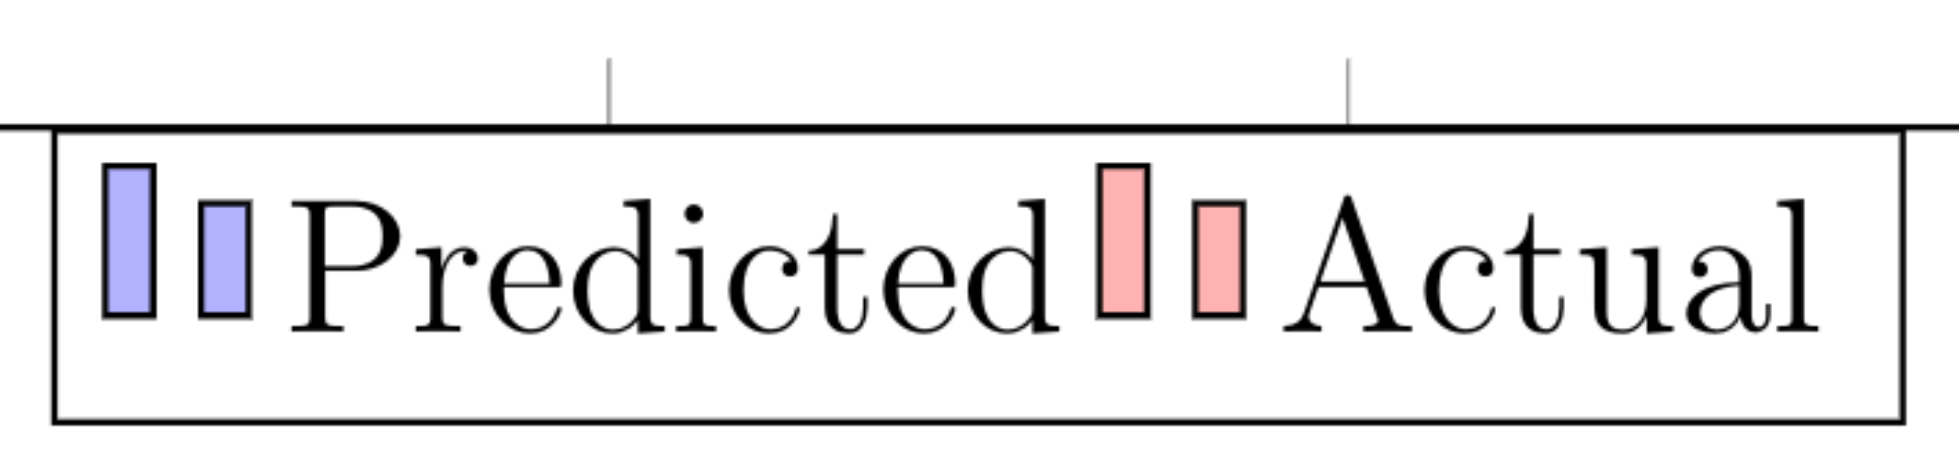
\includegraphics[scale=0.1310]{./figures/legend}}} \end{picture}
    \begin{picture}(0,0) \put(147.35,155.9){\hbox{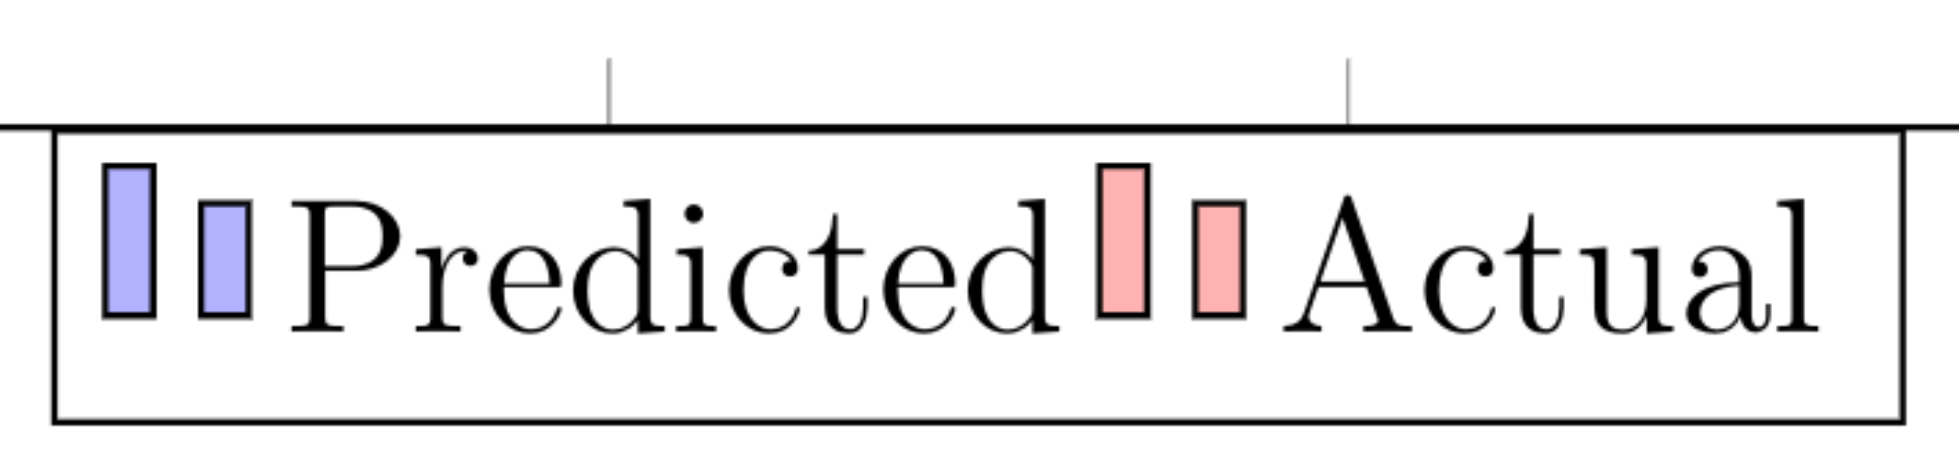
\includegraphics[scale=0.0487]{./figures/legend}}} \end{picture}
    \begin{axis}[
        ybar,
        bar width=.3cm,
        width=0.9\textwidth,
        height=0.45\textwidth,
        symbolic x coords={\texttt{fact}, \texttt{sum\_factors}, \texttt{parse\_files},\texttt{generate\_files},\texttt{add\_footer},\texttt{letter\_count},\texttt{print\_contents},\texttt{count\_vowels},\texttt{separate\_words},\texttt{map\_chars}},
        xtick=data,
        ymode=log,
        ymin=0,ymax=400000,
        xlabel={Programs},
        ylabel={Time (\(\mu s\))},
        xticklabel style={rotate=90},
        tick label style={font=\small},
        xlabel style={yshift=-78pt, font=\large},
        ylabel style={font=\large},
      ]
      \addplot[shift={(2.5,0)}, fill=blue!30!white, error bars/.cd, y dir=both, y explicit] table[x=input_param,y=predicted]{\mydata};
      \addplot[shift={(-2.5,0)}, fill=red!30!white, error bars/.cd, y dir=both, y explicit] table[x=input_param,y=actual, y error plus=actual_order_plus, y error minus=actual_order_minus]{\mydata};
    \end{axis}
  \end{tikzpicture}
  \label{fig:4.1}
  \vspace{-0.5mm}\caption{Comparing \textit{predicted} and \textit{actual runtimes} of Kautuka with 1000 trials --- error bars (unusually) represent one order of magnitude above and below the mean \textit{actual runtime}.}
\end{figure}

\newpage

Measurements were collected on a Dell XPS 15 7590 with the following specifications:

\textbf{Processor} Intel Core i7-9750H CPU @ 2.60GHz × 12

\textbf{Memory} 16 GB 2667 MHz DDR4 RAM

\textbf{OS} Zorin OS 16.2

\textbf{Go Version} go1.19 linux/amd64

The primary source of non-determinism was file-I/O caching. To minimise this effect, we space experiments across set time intervals, separated by redundant operations to clear the cache. These measurements were automated with a bash script, using the Unix \ignore{\texttt{time}} command.

\textbf{Results} In all experiments, our predicted runtime was within an order of magnitude of the true runtime (fig. \hyperref[fig:4.1]{4.1}). One may argue that classifying success as ``within one order of magnitude'' may be too permissive. However, section \hyperref[sec:4.3]{4.3} proves this bound to be sufficiently tight for Kautuka to \textit{consistently outperform} Go. Additionally, there are unpredictable runtime factors (such as caching and inter-process communication) which limit the accuracy of cost analysis.

The programs producing the worst estimates were: \ignore{\texttt{sum\_factors}}, \ignore{\texttt{separate\_words}}, and \ignore{\texttt{map\_chars}}. After investigation, I discovered that the root cause of these inaccuracies were large blocks of non-I/O computations. One explanation for why cost analysis performs worse on these computations is that runtimes of non-I/O operation are orders of magnitude shorter than for I/O operations, measured as a matter of nanoseconds. This requires operations to be executed multiple times in a single run during static profiling, to obtain measurable runtimes. However, repeating operations in such a way makes measurements susceptible to caching effects, reducing the accuracy of static analysis and hence runtime estimates.

However, all other program estimates were accurate, concluding that my \textbf{novel} approach to cost analysis produces \textit{successful} I/O runtime predictions. Since I/O computations dominate runtime in I/O-bound programs (the primary candidates for automatic parallelisation), I constitute this analysis to be a \textit{success}.


\section{Performance on I/O-bound Programs}

\label{sec:4.3}

This section investigates the performance of Kautuka on I/O-bound programs; substantiating claims that Kautuka outperforms Go. Since no existing automatic-parallelisation solutions compile to Go, it would be meaningless to compare their performances with my compiler. Runtime discrepancies would be primarily attributed to the target languages' differing performance, rather than the effectiveness of parallelisation. Thus, the most suitable comparison is with sequential Go, which entails equivalent programming effort to Kautuka (section \hyperref[sec:4.4]{4.4}).

Programmers using the compiler are expected to identify candidate Go files containing expensive (in our case specifically I/O) operations. I performed this methodology on the Kautuka corpus, removing files which fail to satisfy this criteria (\ignore{\texttt{fact}} and \ignore{\texttt{sum\_factors}}). The following benchmarks (fig. \hyperref[fig:4.2]{4.2}) compare the performance of the Kautuka against sequential Go code. By their nature, all chosen Kautuka programs exhibited some degree of parallelisation during execution --- I denote programs containing a combination of both sequential and parallel execution paths with \( \dag \).


\pgfplotstableread[row sep=\\,col sep=&]{
  input_param & kautuka & go & kautuka_err & go_err  \\
  \texttt{parse\_files}\(^\dag\) & 3.93543974 & 6.24607065 & 0.8354047344574917 & 1.4945666661486627\\
  \texttt{generate\_files} & 1.94482751 & 2.65126683 & 0.9112460687334074 & 0.6769222940742172\\
  \texttt{add\_footer}\(^\dag\) & 1.61024851 & 2.5874365499999996 & 1.0762462631630225 & 0.9178685765820006\\
  \texttt{letter\_count} & 1.8470321399999998 & 4.6445662599999995 & 0.6638485104742199 & 1.3971141250272332\\
  \texttt{print\_contents} & 2.3550815299999996 & 3.42348883 & 0.544060833469024 & 0.9825696461239788\\
  \texttt{count\_vowels} & 1.37218422 & 2.52948268 & 0.8774290146103623 & 0.6967561047554715\\
  \texttt{separate\_words} & 5.42705454 & 7.15211727 & 1.0638482023780498 & 1.8217018489778831\\
  \texttt{map\_chars} & 3.04243065 & 4.51591525 & 0.8620350407379548 & 0.931591555199212\\
}\mydata

\begin{figure}[!h]
  \begin{tikzpicture}
    \begin{axis}[
        ybar,
        bar width=.3cm,
        width=0.9\textwidth,
        height=0.45\textwidth,
        symbolic x coords={\texttt{parse\_files}\(^\dag\),\texttt{generate\_files},\texttt{add\_footer}\(^\dag\),\texttt{letter\_count},\texttt{print\_contents},\texttt{count\_vowels},\texttt{separate\_words},\texttt{map\_chars}},
        xtick=data,
        ymin=0,ymax=10,
        xlabel={Programs},
        ylabel={Time (\(s\))},
        xticklabel style={rotate=90},
        tick label style={font=\small},
        xlabel style={yshift=-78pt, font=\large},
        ylabel style={font=\large},
        legend style={at={(0.5,1)},
            anchor=north,legend columns=-1},
      ]
      \addplot[shift={(2.5,0)}, fill=blue!30!white, error bars/.cd, y dir=both, y explicit] table[x=input_param,y=kautuka, y error=kautuka_err]{\mydata};
      \addplot[shift={(-2.5,0)}, fill=red!30!white, error bars/.cd, y dir=both, y explicit] table[x=input_param,y=go, y error=go_err]{\mydata};
      \legend{Kautuka, Go}
    \end{axis}
  \end{tikzpicture}
  \label{fig:4.2}
  \vspace{-0.5mm}\caption{Benchmarking Kautuka against Go. Error bars representing \( \pm \sigma \)}
\end{figure}

\newpage 

\textbf{Results} Our benchmarks show that \textbf{Kautuka consistently outperforms sequential Go}, with performance improvements most pronounced on programs \ignore{\texttt{letter\_count}} and \ignore{\texttt{count\_vowels}}. These programs contain \textit{for-each} loops iterating over file contents, so we deduce that these types of programs exhibit greater performance gains. Overall, these results demonstrate that high-level automatic parallelisation \textit{improves} the performance of I/O-bound programs.


\section{Real-World Compiler Applications}

\label{sec:4.4}

To justify claims that Kautuka integrates into existing workflows, we first illustrate the translation process (from an existing Go file into Kautuka). As is expected with a project of this size, Kautuka lacks some features present in Go such as error handling and file access controls --- which we ignore when translating Go to Kautuka. However, there are no theoretical limitations as to why such features could not be included in the language.

\begin{listing}[!h]
  {
    \captionsetup[figure]{labelformat=empty}%

    \hspace*{-0.5cm}\begin{minipage}{.5\textwidth}
      \begin{minted}{go}
package main 

import ("fmt"; "os") 

func f(x int) {
  for i := 0; i < x; i++ { 
    print(i)
  }
}

func main() { 

  var user_input string 
  fmt.Scan(&user_input)

  user_input_len := len(user_input)

  if user_input_len > 10 { 
    f(user_input_len)
  } else { 
    file, _ := os.OpenFile(user_input,
                           os.O_RDWR, 0777)
    defer file.Close()

    dat, _ := os.ReadFile(file.Name())
    print(string(dat))
  }
}
  \end{minted}
      \begin{center}
        \vspace{-4mm}
        \hspace*{-4mm}{(a) Go}
      \end{center}

      % \label{fig:sample_figure}
    \end{minipage}%
    \begin{minipage}{.5\textwidth}
      \begin{minted}{go}
          package main 
          
          // No explicit imports required 

          func f(x int) {
            for i := 0; i < x; i++ { 
              print(i)
            }
          }
          
          func main() { 

            user_input := input(100) 
            

            user_input_len := len(user_input)

            if user_input_len > 10 { 
              f(user_input_len)
            } else { 
              file := open(user_input)


              
              dat := read(file, 1000)
              print(dat)
            }
          }
      \end{minted}
      \begin{center}
        \vspace{-4mm}
        \hspace*{16mm}{(b) Kautuka}
      \end{center}
    \end{minipage}
  }
  \vspace{2mm}
  \caption{An example I/O-bound program, hand-translated from Go (left) to Kautuka (right).}
  \label{listing:translation}
\end{listing}

\textbf{Results} Listing \hyperref[listing:translation]{1} presents a transliteration of Go to Kautuka with \textit{minimal extra overhead}. Notably, the required annotations (size bounds on I/O inputs) are less strenuous to add than typical parallelisation primitives; the notion of \textit{input sizes} is more grounded than \textit{parallel execution behaviour}, reducing the likelihood of introducing errors. Since Kautuka's syntax is similar to that of Go, and few extra annotations are required, I conclude that Go files can be translated into Kautuka with \textit{minimal effort}.

\newpage 

After translating candidate Go files into Kautuka, the codebase is compiled with my compilation tool. The tool automatically generates parallel Go code from Kautuka files and embeds them into the codebase (deleting Go files once no longer required).

\textbf{Results} Since this tool handles extra complications of a heterogeneous language repository, I conclude that the process of integrating Kautuka into existing Go workflows is \textit{effortless}.

\section{Summary}

\label{sec:4.5}


Kautuka exceeds all success criteria, achieving all core requirements and the majority of extensions listed in Section \hyperref[sec:2.7]{2.7}. Section \hyperref[sec:4.2]{4.2} presents empirical evidence that my novel approach to automatic parallelisation was successful, substantiating the \textit{safety} of side-effect tracking and \textit{accuracy} of cost analysis when implemented in an imperative setting. Our benchmarks reveal that Kautuka outperforms Go on I/O-bound programs (section \hyperref[sec:4.3]{4.3}), highlighting the practicality of high-level automatic parallelisation. Section \hyperref[sec:4.4]{4.4} describes the ease of translating Go files into Kautuka, and how the execution of Kautuka-containing Go codebases requires no additional effort --- showcasing Kautuka's seamless integration into existing workflows.


\addtocontents{lol}{\protect\vspace*{10pt}}
\chapter{Conclusions}
\label{sec:5}

The project was a success. I exceeded all core success criteria and completed the majority of proposed extensions. The project's objective was to create a mid-featured, imperative programming language with a corresponding high-level automatic parallelisation compiler. I implemented both components successfully, ensuring that resultant parallel code was both \textit{safe} and \textit{efficient}. To the best of the author's knowledge, this is the first automatic parallelisation compiler for an imperative language which employs both side-effect tracking and cost analysis. This project highlights potential performance improvements in imperative languages, achieved through high-level automatic parallelisation.

Evaluating my project (using my three research questions as a basis) yielded positive results: 

\begin{enumerate}[leftmargin=8mm]
  \setlength{\itemindent}{-3mm}

  \item \textit{Transfer automatic-parallelisation theory from functional to imperative languages}

  I faced various challenges when implementing automatic-parallelisation theory into an imperative language. To overcome these challenges, I devised \textbf{novel typing rules and algorithms}, which describe how to perform cost analysis in the presence of imperative-style functions and control flow (section \hyperref[sec:3.5]{3.5}). My solutions successfully preserve the \textit{safety} of side-effect tracking and the \textit{accuracy} of cost analysis (section \hyperref[sec:4.2]{4.2}).

  \item \textit{Investigate the performance of high-level parallelisation on I/O-bound programs}
    
  Benchmarking Kautuka against Go on a corpus of I/O-bound programs provided empirical evidence that \textbf{Kautuka outperforms Go} (section \hyperref[sec:4.3]{4.3}).

  \item \textit{Investigate real-world applications of the compiler}
    
  Powerful inferences algorithms (section \hyperref[sec:3.5]{3.5}) allowed me to translate hundreds of lines of Go into Kautuka with \textbf{minimal programmer overhead}. This demonstrates that Kautuka can seamlessly integrate into existing Go workflows using my compiler tooling (section \hyperref[sec:4.4]{4.4}).
  
\end{enumerate}

\section{Lessons Learnt}

\label{sec:5.1}

A significant proportion of the project's focus was on \textit{exploration}, with the majority of time allocated to designing and implementing new algorithms, as opposed to building upon existing work. Whilst rewarding, the research required a substantial initial time investment which I failed to account for in my original timetable. Fortunately, I allocated sufficient slack time to avoid project delays. However, more careful planning would have prevented me deviating from my planned schedule.

I initially intended to implement the entire project with a \textit{spiral development model}. However, I quickly discovered that each compiler stage was heavily dependent on its previous stages, hindering my ability to make incremental iterations. So, despite initial reservations, I used the \textit{waterfall model} for the core project development. I originally avoided this model due to its \textit{inflexibility}, but in reality I found this model to be very effective as all project requirements and deadlines were all fixed in advance. Writing pseudocode for all core components (before starting development) allowed me to commit to design decisions early on, without regretting them at later waterfall stages. This taught me that inflexible development models can be more effective than flexible models in projects where the scope is fixed.

Implementing the type-cost system took significantly longer than expected. The effect system's design was dependent on complex \textit{cost} definitions (appendix \hyperref[sec:C]{C}), which were challenging to implement. On reflection, it would have been beneficial to constrain the core criteria's scope as I now believe it to be ambitious for the time frame provided. Developing a full type-cost system could have been implemented as a stretch goal rather than as part of the core requirements.

\section{Future Work}

\label{sec:5.2}

This project demonstrates that high-level automatic parallelisation\footnote{Using side-effect tracking and cost analysis.} of imperative programs is not only feasible, but also outperforms equivalent sequential code on I/O-bound programs. The natural extension would be to integrate automatic parallelisation into an industry-standard imperative language, such as Go. Common use cases for Go include developing web servers and distributed network applications, which are inherently I/O bound. This suggests that Go is a prime candidate for high-level automatic parallelisation --- with many core ideas of language having already been discussed throughout the dissertation.

Kautuka does not currently support negative numbers, however these pose no fundamental theoretical limitations. Implementing negative numbers requires us to extend the \textit{dependent cost calculus} with \textit{min} and \textit{max} operators. The calculus can be enriched further to support real numbers and operations such as division and modulus. However, doing so would increase the complexity of the calculus, spawning a trade-off between expressivity and the evaluation time of \textit{runtime-cost expressions}. Extending the calculus whilst exploring this trade-off would be an interesting direction for future work.

A more explorative research direction would be to model data-type sizes as probability distributions, rather than relying on upper and lower bounds. This presents new optimisation opportunities, such as branch prediction, not investigated during this project. Probabilistic models would generate more accurate and meaningful runtime estimates, improving the efficiency of produced parallel code. 


% ----------------------------------------------------------------------
%TC:ignore
\newpage

\addcontentsline{toc}{chapter}{\numberline{}Bibliography}
\printbibliography

% ----------------------------------------------------------------------

\appendix

\addtocontents{toc}{\protect\setcounter{tocdepth}{0}}

\chapter{Grammar}

\label{sec:A}

Kautuka is a sequential imperative language defined by the following grammar. Note that this grammar consists of \textit{expressions}, \textit{commands}, and \textit{structures}, and does not make the simplifying assumption to treat commands and structures as unit-type expressions. In Kautuka, semicolons are interchangeable with newline characters.


\begin{fleqn}
        \begin{align*}
                 & \textit{pkg} &  & \hspace*{-4cm}\text{package name}  &  & \\
                 & \textit{fn}  &  & \hspace*{-4cm}\text{function name} &  & \\
                 & x            &  & \hspace*{-4cm}\text{variable name} &  & \\
                 & n            &  & \hspace*{-4cm}\text{integer}       &  & \\
                 & b            &  & \hspace*{-4cm}\text{boolean}       &  & \\
                 & s            &  & \hspace*{-4cm}\text{string}        &  & \\
        \end{align*}


        \vspace{-0.3cm}

        \begin{align*}
                 & \textit{program} \hspace{-0.1cm} & :: & =                                                                                                                                                                &  &                                    \\
                 & \hspace{-0.1cm}                  &    & | \ \ \ \textbf{package} \ \textit{pkg}; \ \textit{func}_1; \, \ldots \, ; \ \textit{func}_n; \ \textbf{func main()} \{ \textit{struct} \, \}                    &  &                                    \\
                 & \hspace{-0.1cm}                  &    &                                                                                                                                                                  &  &                                    \\
                 & \textit{func}    \hspace{-0.1cm} & :: & =                                                                                                                                                                &  &                                    \\
                 & \hspace{-0.1cm}                  &    & | \ \ \ \textbf{func } \textit{fn} \, (x_1: \tau_1, \ldots, x_n: \tau_n ) \: \tau \: \{ \textit{struct} \, \}                                                    &  &                                    \\
                 & \hspace{-0.1cm}                  &    &                                                                                                                                                                  &  &                                    \\
                 & \tau             \hspace{-0.1cm} & :: & =                                                                                                                                                                &  &                                    \\
                 & \hspace{-0.1cm}                  &    & | \ \ \ \textit{int}                                                                                                                                             &  &                                    \\
                 & \hspace{-0.1cm}                  &    & | \ \ \ \textit{bool}                                                                                                                                            &  &                                    \\
                 & \hspace{-0.1cm}                  &    & | \ \ \ \textit{string}                                                                                                                                          &  &                                    \\
                 & \hspace{-0.1cm}                  &    & | \ \ \ /\!\!* \, epsilon \, *\!\!/                                                                                                                              &  & \hspace*{2cm}\text{Unit type}      \\
                 & \hspace{-0.1cm}                  &    & | \ \ \ \textit{file}                                                                                                                                            &  & \hspace*{2cm}\text{File reference} \\
                 & \hspace{-0.1cm}                  &    &                                                                                                                                                                  &  &                                    \\
                 & \textit{struct} \hspace{-0.1cm}  & :: & =                                                                                                                                                                &  & \hspace*{2cm}\text{Structure}      \\
                 & \hspace{-0.1cm}                  &    & | \ \ \ \textbf{if} \ e \, \{ \textit{struct} \, \}                                                                                                              &  &                                    \\
                 & \hspace{-0.1cm}                  &    & | \ \ \ \textbf{if} \ e \, \{ \textit{struct}_1 \, \} \textbf{ else } \{ \textit{struct}_2 \, \}                                                                 &  &                                    \\
                 & \hspace{-0.1cm}                  &    & | \ \ \ \textbf{if} \ e_1 \, \{ \textit{struct}_1 \, \} \textbf{ else if } e_2 \, \{ \textit{struct}_2 \, \} \ldots \, \textbf{else } \{ \textit{struct}_n \, \} &  &                                    \\
                 & \hspace{-0.1cm}                  &    & | \ \ \ \textbf{for} \ x := e_1; \, x < e_2; \, x \! + \! + \; \{ \textit{struct} \, \}                                                                          &  &                                    \\
                 & \hspace{-0.1cm}                  &    & | \ \ \ \textbf{for} \ x := \textbf{range} \ e \: \{ \textit{struct} \,  \}                                                                                      &  &                                    \\
                 & \hspace{-0.1cm}                  &    & | \ \ \ \{ \textit{struct} \, \}                                                                                                                                 &  & \hspace*{2cm}\text{Code block}     \\
                 & \hspace{-0.1cm}                  &    & | \ \ \ \textit{struct}_1; \, \textit{struct}_2                                                                                                                  &  &                                    \\
                 & \hspace{-0.1cm}                  &    & | \ \ \ \textit{command}_1; \, \ldots \, ; \textit{command}_n                                                                                                    &  &                                    \\
        \end{align*}

        \begin{align*}
                 & \textit{command} \hspace{-0.1cm} & :: & =                                     &  &                                                        \\
                 & \hspace{-0.1cm}                  &    & | \ \ \ x := e                        &  & \hspace*{5.6cm}\text{Declaration (with assignment)}    \\
                 & \hspace{-0.1cm}                  &    & | \ \ \ \textbf{var} \ x              &  & \hspace*{5.6cm}\text{Declaration (without assignment)} \\
                 & \hspace{-0.1cm}                  &    & | \ \ \ \textbf{var} \ x \ \tau       &  & \hspace*{5.6cm}\text{Declaration (with explicit type)} \\
                 & \hspace{-0.1cm}                  &    & | \ \ \ x = e                         &  & \hspace*{5.6cm}\text{Assignment}                       \\
                 & \hspace{-0.1cm}                  &    & | \ \ \ \textit{fn}(e_1, \ldots, e_n) &  & \hspace*{5.6cm}\text{Call (user-defined) func}         \\
                 & \hspace{-0.1cm}                  &    & | \ \ \ \textbf{return} \ e           &  & \hspace*{5.6cm}\text{Return expr from func}            \\
                 &                                  &    & | \ \ \ \textbf{print}(e)             &  & \hspace*{5.6cm}\text{Console print}                    \\
                 &                                  &    & | \ \ \ \textbf{write}(e_1, e_2)      &  & \hspace*{5.6cm}\text{File write (overwrite contents)}  \\
                 &                                  &    & | \ \ \ \textbf{append}(e_1, e_2)     &  & \hspace*{5.6cm}\text{File append}                      \\
                 & \hspace{-0.1cm}                  &    &                                       &  &                                                        \\
                 & \textit{e} \hspace{-0.1cm}       & :: & =                                     &  &                                                        \\
                 & \hspace{-0.1cm}                  &    & | \ \ \ \textit{unop } e              &  &                                                        \\
                 & \hspace{-0.1cm}                  &    & | \ \ \ e_1 \textit{ binop } e_2      &  &                                                        \\
                 & \hspace{-0.1cm}                  &    & | \ \ \ n                             &  & \hspace*{5.6cm}\text{Integer}                          \\
                 & \hspace{-0.1cm}                  &    & | \ \ \ b                             &  & \hspace*{5.6cm}\text{Boolean}                          \\
                 & \hspace{-0.1cm}                  &    & | \ \ \ s                             &  & \hspace*{5.6cm}\text{String literal}                   \\
                 & \hspace{-0.1cm}                  &    & | \ \ \ x                             &  & \hspace*{5.6cm}\text{Variable read}                    \\
                 & \hspace{-0.1cm}                  &    & | \ \ \ (e)                           &  &                                                        \\
                 &                                  &    & | \ \ \ \textbf{input}(n)             &  & \hspace*{5.6cm}\text{Console input (lower bound)}      \\
                 &                                  &    & | \ \ \ \textbf{input}(n_1, n_2)      &  & \hspace*{5.6cm}\text{Console input (both bounds)}      \\
                 &                                  &    & | \ \ \ \textbf{open}(e)              &  & \hspace*{5.6cm}\text{File open (unspecified group)}    \\
                 &                                  &    & | \ \ \ \textbf{open}(e, n)           &  & \hspace*{5.6cm}\text{File open (specified group)}      \\
                 &                                  &    & | \ \ \ \textbf{read}(e, n)           &  & \hspace*{5.6cm}\text{File read (lower bound)}          \\
                 &                                  &    & | \ \ \ \textbf{read}(e, n_1, n_2)    &  & \hspace*{5.6cm}\text{File read (both bounds)}          \\
                 &                                  &    &                                       &  &                                                        \\
                 & \textit{unop}\hspace{-0.1cm}     & :: & =                                     &  &                                                        \\
                 &                                  &    & | \ \ \ !                             &  & \hspace*{5.6cm}\text{Not}                              \\
                 &                                  &    & | \ \ \ -                             &  & \hspace*{5.6cm}\text{Negation}                         \\
                 &                                  &    &                                       &  &                                                        \\
                 & \textit{binop}\hspace{-0.1cm}    & :: & =                                     &  &                                                        \\
                 &                                  &    & | \ \ \ +                             &  & \hspace*{5.6cm}\text{Addition}                         \\
                 &                                  &    & | \ \ \ *                             &  & \hspace*{5.6cm}\text{Multiplication}                   \\
                 &                                  &    & | \ \ \ -                             &  & \hspace*{5.6cm}\text{Subtraction}                      \\
                 &                                  &    & | \ \ <                               &  & \hspace*{5.6cm}\text{Less than}                        \\
                 &                                  &    & | \ \ <=                              &  & \hspace*{5.6cm}\text{Less than equal}                  \\
                 &                                  &    & | \ \ >                               &  & \hspace*{5.6cm}\text{Greater than}                     \\
                 &                                  &    & | \ \ >=                              &  & \hspace*{5.6cm}\text{Greater than equal}               \\
                 &                                  &    & | \ \ ==                              &  & \hspace*{5.6cm}\text{Equal}                            \\
                 &                                  &    & | \ \ \ !=                            &  & \hspace*{5.6cm}\text{Not equal}                        \\
                 &                                  &    & | \ \ \ \&\&                          &  & \hspace*{5.6cm}\text{And}                              \\
                 &                                  &    & | \ \ \ | |                           &  & \hspace*{5.6cm}\text{Or}                               \\
        \end{align*}

\end{fleqn}


\newpage

\chapter{Side-Effect System}

\label{sec:B}

\section*{Typing Judgement}

The side-effect system typing judgement takes the form:

\[ \Gamma^\textrm{se} \vdash e : \tau^\textrm{se}, f \]

where

\vspace{2mm}

\( \tau^\textrm{se} \): base types enriched with latent side effects

\( f \in \mathscr{P}(\mathit{Side\text{-}Effect}) \): side-effect set

\( \tau^\textrm{se}, f \): representation of immediate and latent side effects

\( \Gamma^\textrm{se} \): mapping from variables to \( \tau^\textrm{se} \)

\vspace{-1mm}

\section*{Typing Rules}

\vspace{-3mm}

For brevity, we write \( \tau^\textrm{se} \) as \( \tau \) and \( \Gamma^\textrm{se} \) as \( \Gamma \). Note that these rules also capture file-reference tracking if we consider file references with different identifiers and groups (e.g. \( \textit{file\_ref}\,(i_1, g_1) \) and \( \textit{file\_ref}\,(i_2, g_2) \)) to be of the same type.
\vspace{3mm}

% int, bool, string 

\hspace*{-1.5cm}\begin{minipage}{.33\paperwidth}
  \begin{prooftree}
    \AxiomC{}
    \RightLabel{\((\emph{int})\)}
    \UnaryInfC{\(\Gamma \vdash n : \textit{int}, \{ \} \)}
  \end{prooftree}
\end{minipage}%
\hspace*{-1cm}\begin{minipage}{.33\paperwidth}
  \begin{prooftree}
    \AxiomC{}
    \RightLabel{\((\emph{bool})\)}
    \UnaryInfC{\(\Gamma \vdash b : \textit{bool}, \{ \} \)}
  \end{prooftree}
\end{minipage}
\hspace*{-1cm}\begin{minipage}{.33\paperwidth}
  \begin{prooftree}
    \AxiomC{}
    \RightLabel{\((\emph{string})\)}
    \UnaryInfC{\(\Gamma \vdash s : \textit{string}, \{ \} \)}
  \end{prooftree}
\end{minipage}

% add, multiply, subtract, concat

\vspace{3mm}

\hspace*{-1.5cm}\begin{minipage}{.5\paperwidth}
  \begin{prooftree}
    \AxiomC{\(\Gamma \vdash e_1 : \textit{int}, f_1\)}
    \AxiomC{\(\Gamma \vdash e_2 : \textit{int}, f_2\)}
    \RightLabel{\((\emph{add})\)}
    \BinaryInfC{\(\Gamma \vdash e_1 + e_2 : \textit{int}, f_1 \cup f_2\)}
  \end{prooftree}
\end{minipage}%
\hspace*{-1.3cm}\begin{minipage}{.5\paperwidth}
  \begin{prooftree}
    \AxiomC{\(\Gamma \vdash e_1 : \textit{int}, f_1\)}
    \AxiomC{\(\Gamma \vdash e_2 : \textit{int}, f_2\)}
    \RightLabel{\((\emph{mult})\)}
    \BinaryInfC{\(\Gamma \vdash e_1 * e_2 : \textit{int}, f_1 \cup f_2\)}
  \end{prooftree}
\end{minipage}

\vspace{2mm}

\hspace*{-1.5cm}\begin{minipage}{.5\paperwidth}
  \begin{prooftree}
    \AxiomC{\(\Gamma \vdash e_1 : \textit{int}, f_1\)}
    \AxiomC{\(\Gamma \vdash e_2 : \textit{int}, f_2\)}
    \RightLabel{\((\emph{sub})\)}
    \BinaryInfC{\(\Gamma \vdash e_1 - e_2 : \textit{int}, f_1 \cup f_2\)}
  \end{prooftree}
\end{minipage}%
\hspace*{-1.3cm}\begin{minipage}{.5\paperwidth}
  \begin{prooftree}
    \AxiomC{\(\Gamma \vdash e_1 : \textit{string}, f_1\)}
    \AxiomC{\(\Gamma \vdash e_2 : \textit{string}, f_2\)}
    \RightLabel{\((\emph{concat})\)}
    \BinaryInfC{\(\Gamma \vdash e_1 + e_2 : \textit{string}, f_1 \cup f_2\)}
  \end{prooftree}
\end{minipage}

% lt, le, gt, ge, and, or, not, eq, neq, () 

\vspace{2mm}

\hspace*{-1.5cm}\begin{minipage}{.5\paperwidth}
  \begin{prooftree}
    \AxiomC{\(\Gamma \vdash e_1 : \textit{int}, f_1\)}
    \AxiomC{\(\Gamma \vdash e_2 : \textit{int}, f_2\)}
    \RightLabel{\( ( < ) \)}
    \BinaryInfC{\(\Gamma \vdash e_1 < e_2 : \textit{bool}, f_1 \cup f_2\)}
  \end{prooftree}
\end{minipage}%
\hspace*{-1.3cm}\begin{minipage}{.5\paperwidth}
  \begin{prooftree}
    \AxiomC{\(\Gamma \vdash e_1 : \textit{int}, f_1\)}
    \AxiomC{\(\Gamma \vdash e_2 : \textit{int}, f_2\)}
    \RightLabel{\( ( \le ) \)}
    \BinaryInfC{\(\Gamma \vdash e_1 <= e_2 : \textit{bool}, f_1 \cup f_2\)}
  \end{prooftree}
\end{minipage}

\vspace{2mm}

\hspace*{-1.5cm}\begin{minipage}{.5\paperwidth}
  \begin{prooftree}
    \AxiomC{\(\Gamma \vdash e_1 : \textit{int}, f_1\)}
    \AxiomC{\(\Gamma \vdash e_2 : \textit{int}, f_2\)}
    \RightLabel{\( ( > ) \)}
    \BinaryInfC{\(\Gamma \vdash e_1 > e_2 : \textit{bool}, f_1 \cup f_2\)}
  \end{prooftree}
\end{minipage}%
\hspace*{-1.3cm}\begin{minipage}{.5\paperwidth}
  \begin{prooftree}
    \AxiomC{\(\Gamma \vdash e_1 : \textit{int}, f_1\)}
    \AxiomC{\(\Gamma \vdash e_2 : \textit{int}, f_2\)}
    \RightLabel{\( ( \ge ) \)}
    \BinaryInfC{\(\Gamma \vdash e_1 >= e_2 : \textit{bool}, f_1 \cup f_2\)}
  \end{prooftree}
\end{minipage}

\vspace{2mm}

\hspace*{-1.5cm}\begin{minipage}{.5\paperwidth}
  \begin{prooftree}
    \AxiomC{\(\Gamma \vdash e_1 : \textit{int}, f_1\)}
    \AxiomC{\(\Gamma \vdash e_2 : \textit{int}, f_2\)}
    \RightLabel{\( ( = ) \)}
    \BinaryInfC{\(\Gamma \vdash e_1 == e_2 : \textit{bool}, f_1 \cup f_2\)}
  \end{prooftree}
\end{minipage}%
\hspace*{-1.3cm}\begin{minipage}{.5\paperwidth}
  \begin{prooftree}
    \AxiomC{\(\Gamma \vdash e_1 : \textit{int}, f_1\)}
    \AxiomC{\(\Gamma \vdash e_2 : \textit{int}, f_2\)}
    \RightLabel{\( ( \neq ) \)}
    \BinaryInfC{\(\Gamma \vdash e_1 \: !\!= e_2 : \textit{bool}, f_1 \cup f_2\)}
  \end{prooftree}
\end{minipage}

\vspace{2mm}

\hspace*{-1.5cm}\begin{minipage}{.5\paperwidth}
  \begin{prooftree}
    \AxiomC{\(\Gamma \vdash e_1 : \textit{bool}, f_1\)}
    \AxiomC{\(\Gamma \vdash e_2 : \textit{bool}, f_2\)}
    \RightLabel{\( (\land) \)}
    \BinaryInfC{\(\Gamma \vdash e_1 \: \&\& \: e_2 : \textit{bool}, f_1 \cup f_2\)}
  \end{prooftree}
\end{minipage}%
\hspace*{-1.3cm}\begin{minipage}{.5\paperwidth}
  \begin{prooftree}
    \AxiomC{\(\Gamma \vdash e_1 : \textit{bool}, f_1\)}
    \AxiomC{\(\Gamma \vdash e_2 : \textit{bool}, f_2\)}
    \RightLabel{\( (\lor) \)}
    \BinaryInfC{\(\Gamma \vdash e_1 \: || \: e_2 : \textit{bool}, f_1 \cup f_2\)}
  \end{prooftree}
\end{minipage}

\vspace{1mm}

\hspace*{-1.5cm}\begin{minipage}{.5\paperwidth}
  \begin{prooftree}
    \AxiomC{\(\Gamma \vdash e : \textit{bool}, f\)}
    \RightLabel{\( (\neg) \)}
    \UnaryInfC{\(\Gamma \vdash \: ! e : \textit{bool}, f \)}
  \end{prooftree}
\end{minipage}%
\hspace*{-1.3cm}\begin{minipage}{.5\paperwidth}
  \begin{prooftree}
    \AxiomC{\(\Gamma \vdash e : \tau, f\)}
    \RightLabel{\((\emph{paren})\)}
    \UnaryInfC{\(\Gamma \vdash ( e ) : \tau, f \)}
  \end{prooftree}
\end{minipage}

% x, =, :=, (_ = e)

\hspace*{-1.9cm}\begin{minipage}{.5\paperwidth}
  \vspace{4mm}
  \begin{prooftree}
    \AxiomC{}
    \RightLabel{\((\emph{var-read})\)}
    \UnaryInfC{\(\Gamma[x : \tau] \vdash x : \tau, \{\textsc{r}, \text{var}(x)\}\)}
  \end{prooftree}
\end{minipage}%
\hspace*{-1.7cm}\begin{minipage}{.5\paperwidth}
  \begin{prooftree}
    \AxiomC{\(\Gamma \vdash e_1 : \tau_1, f_1 \)}
    \AxiomC{\((x: \tau_1), \Gamma \vdash e_2 : \tau_2, f_2 \)}
    \RightLabel{\((\emph{var-declare})\)}
    \BinaryInfC{\(\Gamma \vdash x := e_1; \, e_2 : \tau_2, (f_1 \cup f_2) \)}
  \end{prooftree}
\end{minipage}

\begin{prooftree}
  \AxiomC{\(\Gamma \vdash e_1 : \tau_1, f_1 \)}
  \AxiomC{\((x: \tau_1), \Gamma \vdash e_2 : \tau_2, f_2 \)}
  \RightLabel{\((\emph{var-assign})\)}
  \BinaryInfC{\(\Gamma[x : \tau_1] \vdash x = e_1; \, e_2 : \tau_2, (f_1 \cup f_2 \cup \{(\textsc{w}, \text{var}(x))\}) \)}
\end{prooftree}

% (e1; e2), {}  

\hspace*{-1.8cm}\begin{minipage}{.5\paperwidth}
  \begin{prooftree}
    \AxiomC{\( \Gamma \vdash e_1 : \textit{unit}, f_1 \) }
    \AxiomC{\( \Gamma \vdash e_2 : \tau, f_2 \) }
    \RightLabel{\((\emph{seq})\)}
    \BinaryInfC{\(\Gamma \vdash e_1; e_2 : \tau, f_1 \cup f_2 \)}
  \end{prooftree}
\end{minipage}%
\hspace*{-1.6cm}\begin{minipage}{.5\paperwidth}
  \begin{prooftree}
    \AxiomC{\( \Gamma \vdash e : \textit{unit}, f \)}
    \RightLabel{\((\emph{block}\,\footnotemark{})\)}
    \UnaryInfC{\(\Gamma \vdash \{ e \}_{ \{ x, y, \ldots, z \} } : \textit{unit}, f \setminus \{ x, y, \ldots, z \} \)}
  \end{prooftree}
\end{minipage}

% if, if-else, for-loop, for-each 

\begin{prooftree}
  \AxiomC{\( \Gamma \vdash e_1 : \textit{bool}, f_1 \)}
  \AxiomC{\( \Gamma \vdash e_2 : \textit{unit}, f_2 \)}
  \RightLabel{\((\emph{if})\)}
  \BinaryInfC{\(\Gamma \vdash \textrm{if } e_1 \; \{ \, e_2 \, \} : \textit{unit}, (f_1 \cup f_2) \)}
\end{prooftree}

\begin{prooftree}
  \AxiomC{\( \Gamma \vdash e_1 : \textit{bool}, f_1 \)}
  \AxiomC{\( \Gamma \vdash e_2 : \textit{unit}, f_2 \)}
  \AxiomC{\( \Gamma \vdash e_3 : \textit{unit}, f_3 \)}
  \RightLabel{\((\emph{if-else})\)}
  \TrinaryInfC{\(\Gamma \vdash \textrm{if } e_1 \; \{ \, e_2 \, \} \textrm{ else } \{ \, e_3 \, \} : \textit{unit}, (f_1 \cup f_2 \cup f_3) \)}
\end{prooftree}

\begin{prooftree}
  \AxiomC{\( \Gamma \vdash e_1 : \textit{int}, f_1 \)}
  \AxiomC{\( \Gamma \vdash e_2 : \textit{int}, f_2 \)}
  \AxiomC{\( \Gamma \vdash e_3 : \textit{unit}, f_3 \)}
  \RightLabel{\((\emph{for-loop})\)}
  \TrinaryInfC{\(\Gamma \vdash \textrm{for } x := e_1 \, ; \, x < e_2 \, ; \, x \! + \! + \; \{ \, e_3 \, \} : \textit{unit}, (f_1 \cup f_2 \cup f_3) \)}
\end{prooftree}

\begin{prooftree}
  \AxiomC{\( \Gamma \vdash e_1 : \textit{string}, f_1 \)}
  \AxiomC{\( (x: \textit{string}), \Gamma \vdash e_2 : \textit{unit}, f_2 \)}
  \RightLabel{\((\emph{for-each})\)}
  \BinaryInfC{\(\Gamma \vdash \textrm{for } x := \text{range } e_1 \, \{ \, e_2 \, \} : \textit{unit}, (f_1 \cup f_2) \)}
\end{prooftree}

% print, input-1, input-2, open, read, write, append 

\hspace*{-1.5cm}\begin{minipage}{.5\paperwidth}
  \begin{prooftree}
    \AxiomC{\( \Gamma \vdash e : \textit{string}, f \)}
    \RightLabel{\((\emph{print})\)}
    \UnaryInfC{\(\Gamma \vdash \textrm{print}(e) : \textit{unit}, f \cup \{(\textsc{w}, \text{console})\}\)}
  \end{prooftree}
\end{minipage}%
\hspace*{-1.3cm}\begin{minipage}{.5\paperwidth}
  \begin{prooftree}
    \AxiomC{ \( \Gamma \vdash n : \textit{int}, \{ \} \) }
    \RightLabel{\((\emph{input-1})\)}
    \UnaryInfC{\(\Gamma \vdash \textrm{input}(n) : \textit{string}, \{(\textsc{w}, \text{console})\}\)}
  \end{prooftree}
\end{minipage}

\vspace{3mm}

\hspace*{-1cm}\begin{minipage}{.5\paperwidth}
  \begin{prooftree}
    \AxiomC{ \( \Gamma \vdash n_1 : \textit{int}, \{ \} \) }
    \AxiomC{ \( \hspace{-6mm}\Gamma \vdash n_2 : \textit{int}, \{ \} \) }
    \AxiomC{\( \hspace{-3mm}\hspace{-1.8mm}n_1 \leq n_2 \)}
    \RightLabel{\((\emph{input-2})\)}
    \TrinaryInfC{\(\Gamma \vdash \textrm{input}(n_1, n_2) : \textit{string}, \{(\textsc{w}, \text{console})\}\)}
  \end{prooftree}
\end{minipage}%
\hspace*{-1.3cm}\begin{minipage}{.5\paperwidth}
  \begin{prooftree}
    \AxiomC{\( \Gamma \vdash e : \textit{string}, f \)}
    \RightLabel{\((\emph{open-1}\,\footnotemark{})\)}
    \UnaryInfC{\(\Gamma \vdash \textrm{open}(e) : \textit{file\_ref}\,(i', g'), f \)}
  \end{prooftree}
\end{minipage}

\addtocounter{footnote}{-1}

\vspace{3mm}

\hspace*{-2.2cm}\begin{minipage}{.5\paperwidth}
  \begin{prooftree}
    \AxiomC{\( \Gamma \vdash e : \textit{string}, f \)}
    \AxiomC{\( \Gamma \vdash n : \textit{int}, \{ \} \)}
    \RightLabel{\((\emph{open-2}\,\footnotemark{})\)}
    \BinaryInfC{\(\Gamma \vdash \textrm{open}(e, n) : \textit{file\_ref}\,(i', n), f \)}
  \end{prooftree}
\end{minipage}%
\hspace*{-1.1cm}\begin{minipage}{.5\paperwidth}
  \begin{prooftree}
    \AxiomC{\( \Gamma \vdash e : \textit{file\_ref}\,(i, g), f \)}
    \AxiomC{\( \Gamma \vdash n : \textit{int}, \{ \} \)}
    \RightLabel{\((\emph{file-read-1})\)}
    \BinaryInfC{\(\Gamma \vdash \textrm{read}(e, n) : \textit{string}, f \cup \{(\textsc{r}, \text{file}(i, g))\}\)}
  \end{prooftree}
\end{minipage}

\vspace{3mm}

\begin{prooftree}
  \AxiomC{\( \Gamma \vdash e : \textit{file\_ref}\,(i, g), f \)}
  \AxiomC{\( \Gamma \vdash n_1 : \textit{int}, \{ \} \)}
  \AxiomC{\( \Gamma \vdash n_2: \textit{int}, \{ \} \)}
  \AxiomC{\( \hspace{-1.8mm}n_1 \leq n_2 \)}
  \RightLabel{\((\emph{file-read-2})\)}
  \QuaternaryInfC{\(\Gamma \vdash \textrm{read}(e, n_1, n_2) : \textit{string}, f \cup \{(\textsc{r}, \text{file}(i, g))\}\)}
\end{prooftree}

\vspace{0.5mm}

\begin{prooftree}
  \AxiomC{\( \Gamma \vdash e_1 : \textit{file\_ref}\,(i, g), f_1 \)}
  \AxiomC{\( \Gamma \vdash e_2 : \textit{string}, f_2 \)}
  \RightLabel{\((\emph{file-write})\)}
  \BinaryInfC{\(\Gamma \vdash \textrm{write}(e_1, e_2) : \textit{unit}, (f_1 \cup f_2 \cup \{(\textsc{w}, \text{file}(i, g))\}) \)}
\end{prooftree}

\vspace{0.5mm}


\begin{prooftree}
  \AxiomC{\( \Gamma \vdash e_1 : \textit{file\_ref}\,(i, g), f_1 \)}
  \AxiomC{\( \Gamma \vdash e_2 : \textit{string}, f_2 \)}
  \RightLabel{\((\emph{file-append})\)}
  \BinaryInfC{\(\Gamma \vdash \textrm{append}(e_1, e_2) : \textit{unit}, (f_1 \cup f_2 \cup \{(\textsc{w}, \text{file}(i, g))\}) \)}
\end{prooftree}

% func-def, func-call, return

\vspace{-2mm}

\begin{prooftree}
  \AxiomC{\(x_1: \tau_1, \, \ldots \,, x_n : \tau_n, \Gamma \vdash e : \tau, f\)}
  \AxiomC{\((g: \tau_1 * \cdots * \tau_n \xrightarrow{f} \tau), \Gamma \vdash e^\prime : \tau^\prime, f^\prime\)}
  \RightLabel{\((\emph{def-func})\)}
  \BinaryInfC{\(\Gamma \vdash (\textrm{def } g(x_1: \tau_1, \, \ldots \, , x_n: \tau_n) \; \tau \; \{ \, e \, \} ; \, e^\prime) : \tau^\prime, f^\prime \)}
\end{prooftree}

\begin{prooftree}
  \AxiomC{\(\Gamma(g) = \tau_1 * \cdots * \tau_n \xrightarrow{f} \tau \)}
  \AxiomC{\( \Gamma \vdash e_1 : \tau_1, f_1 \)}
  \AxiomC{\( \hspace{-2.5mm} \cdots \hspace{-2.5mm} \)}
  \AxiomC{\( \Gamma \vdash e_n : \tau_n, f_n \)}
  \RightLabel{\((\emph{apply-func})\)}
  \QuaternaryInfC{\( \Gamma \vdash g(e_1, \ldots, e_n) : \tau, (f \cup f_1 \cup \cdots \cup f_n) \)}
\end{prooftree}

\vspace{5mm}

\addtocounter{footnote}{-1}
\addtocounter{footnote}{-1}

\stepcounter{footnote}\footnotetext{All scopes remove local-variable side effects. However,  we only apply this rule to the \( (\emph{blocks}) \) for brevity.}
\stepcounter{footnote}\footnotetext{Where \( i' \) represents a fresh identifier and \( g' \) represents a fresh group.}


\newpage

\chapter{Type-Cost System}

\label{sec:C}

\section*{Cost Definitions}

In this section, we provide a full description of the \textit{dependent cost calculus}: the representation of costs in Kautuka which depend on unknown input sizes. The theoretical definitions mirror my code implementation.

The set \( \textit{Var} \) contains all program variables, specifically referring to \textit{function inputs} in this context. When evaluated (dynamically), the value of a variable is its \textit{size}. Exponentiated variables are represented with the set \( \textit{Exp\text{-}Var} = \mathit{Var} \times \mathbb{N} \), noting that exponents are constrained to \textit{integers}\footnote{The language does not contain exponentiation operators, and we assume that loops do not produce exponential behaviour (section \hyperref[sec:2.5.1]{2.5.1}).}. This set contains elements of the form \( (x, n) \), representing exponentiated variables \( x^n \). \textit{Variable terms} are the product of an arbitrary number of integers and variables, and are written in the form \( i \cdot x^m y^n \cdots z^p \) (where \(i, m, n, \ldots, p \in \mathbb{N} \) and \(x, y, \ldots, z \in \textit{Var} \)). This set is defined as \( {\mathit{Var\text{-}Term} = \mathbb{N} \times \mathscr{P}(\mathit{Exp\text{-}Var})} \). These terms are summed to produce \textit{polynomial terms} (\( \mathscr{P}(\mathit{Var\text{-}Term}) \)) of the form \( i \cdot {w^m} \cdots {x^n} + \cdots + j \cdot {y^p} \cdots {z^q} \). Note that this is simply a set-theoretical definition of \textit{polynomial expressions}. In our language, polynomial terms are sufficient to describe all costs. A cost bound can be constructed with two polynomial terms (\( \mathit{Poly\text{-}Term}    \times \mathit{Poly\text{-}Term} \)), representing the upper and lower bounds: \( { \bound{\textit{lower\_cost}}{\textit{upper\_cost}} } \). So a cost bound \( \bound{l}{u} \) contains the two \textit{polynomial terms} \( l \) and \( u \).



\begin{align*}
  \mathit{Var}               & = \{x, y, z, \ldots \}                                          & x                                                                \\
  \mathit{Exp\text{-}Var}    & = \mathit{Var}\times \mathbb{N}                                 & x^n                                                              \\
  \mathit{Var\text{-}Term}   & = \mathbb{N} \times \mathscr{P}(\mathit{Exp\text{-}Var})        & i \cdot x^m y^n \cdots z^p                                       \\
  \mathit{Poly\text{-}Term}  & = \mathscr{P}(\mathit{Var\text{-}Term})                         & i \cdot {w^m} \cdots {x^n} + \cdots + j \cdot {y^p} \cdots {z^q} \\
  \mathit{Cost\text{-}Bound} & = \mathit{Poly\text{-}Term}    \times \mathit{Poly\text{-}Term} & \bound{\textit{lower\_cost}}{\textit{upper\_cost}}
\end{align*}

\section*{Cost Operations}

Given two polynomial terms \( p_1 \) and \( p_2 \), we can perform the following operations: \( {(p_1 + p_2)}, \, {(p_1 - p_2)}, \, {(p_1 \cdot p_2)}, \, {\max(p_1, p_2)}, \, {\min(p_1, p_2)} \).

Two \textit{variable terms} are considered to be \textit{matching} if they contain the same variables with the same exponents (but potentially differing integer coefficients). The operations \( {(p_1 + p_2)}, {(p_1 - p_2)}, {(p_1 \cdot p_2)} \) are defined as expected (treating the polynomial terms as if they were polynomial expressions). For example, \( (8x + 3xy^2) + (3x + 2x^2) = 11x + 3xy^2 + 2x^2 \) and \( (2x + 1) \cdot (3y) = 6xy + 3y\). This is implemented as follows:

When adding \( p_1 + p_2 \), we join together variable terms containing the same variables (for example \( 3xy + 5xy \) becomes \( 8xy \)). This is implemented by scanning all variable terms in \( p_1 \) and \( p_2 \) and checking if they are matching. If they are, then we decompose the variable terms into their constituent parts: the variables \( w^m \cdots x^n \) (shared between the terms) and the two coefficients of each term \( i_1 \) and \( i_2 \). We add \( (i_1 + i_2) \cdot w^m \cdots x^n \) to the total (initially 0). Once we have identified all matching pairs, we then add all remaining variable terms in \( p_1 \) and \( p_2 \) to the result. Algorithm \hyperref[alg:two]{2} presents an algorithm to implement this.

\begin{algorithm}[hbt!]
  \caption{Addition of Polynomial Terms}\label{alg:two}
  \KwData{\( p_1, p_2 \)}
  \KwResult{\( p \)}

  \BlankLine

  \( p \gets 0 \)\;

  \BlankLine

  \For{\((i \cdot w^m \cdots x^n) \in p_1\)} {

    \BlankLine

    \( \textit{found\_matching} \gets \textit{false} \)\;

    \BlankLine

    \For{\((j \cdot y^p \cdots z^q) \in p_2\)} {
      \If{\text{is\_matching}\(( (i \cdot w^m \cdots x^n), (j \cdot y^p \cdots z^q) )\)}{
        \( p \gets p \cup \{ ((i + j) \cdot w^m \cdots x^n) \} \)\;
        \( p_2 \gets p_2 \backslash \{ (j \cdot y^p \cdots z^q) \} \)\;
        \( \textit{found\_matching} \gets \textit{true} \)\;
      }
    }
    \If{\(\lnot \textit{found\_matching} \)} {
      \( p \gets p \cup \{ (i \cdot w^m \cdots x^n) \} \)\;
    }
  }

  \( p \gets p \cup p_2 \)\;

\end{algorithm}

Subtraction follows similarly, where we instead add \( ((i - j) \cdot w^m \cdots x^n) \) to the result.

The multiplication of two \textit{variable terms} \( v_1 \cdot v_2 \) is defined as multiplying their coefficients and unioning their exponentiated variables. However, if any of the variables in \( v_1 \) and \( v_2 \) match, then their exponents are added together during this process. This allows us to define the multiplication of two polynomial terms \( p_1 \cdot p_2 \): for all \( v_1 \in p_1 \) and \( v_2 \in p_2 \), we add \( v_1 \cdot v_2 \) to an initially empty result.

The minimum and maximum of two polynomial terms are defined conservatively. We say that the maximum of two different unknown variables \( x \) and \( y \) is \( x + y \). But if two variable terms contain the same variables (and exponents) then we simply take the maximum of the coefficients, \( {\max(3xy^2 + 2x, 2xy^2 + 4y) = 3xy^2 + 2x + 4y} \).

However, finding the minimum of two abstract terms is not possible with our current calculus. Taking \( x - y \) does not work as we cannot ensure that the result is non-negative. One approach to this problem would be to add the \( \min \) operator into the calculus, however extending the calculus in this way is outside the scope of this project. Another solution would be to approximate the minimum with an average of the two inputs, however our calculus only supports integers (and does not support rounding operations). Hence, we opt for an even cruder approach of approximating the minimum of two variables. We apply the same approach as calculating the maximum, however we take the minimum of coefficients rather than the maximum, \( {\min(3xy^2 + 2x, 2xy^2 + 2x + 4y) = 2xy^2 + 2x + 4y} \). While this is not an accurate approximation, it does ensure that the result is always positive and is more meaningful than just returning \( 0 \). Surprisingly, the inaccuracy of this bound does not have a large impact overall (as shown by the results of section \hyperref[sec:4.2]{4.2}). The purpose of these bounds are to approximate the \textit{magnitude} of costs, rather than to produce accurate estimates. This approach succeeds in that goal, however it is possible to construct adversarial inputs where this approach fails to produce reasonable estimates. We discuss the alternative approaches in further detail in section \hyperref[sec:5.2]{5.2}.

From these operations, we can define the cost definitions presented in the section \hyperref[sec:3.5.1]{3.5.1}:

\begin{align*}
  c_1 + c_2         & \triangleq \bound{l_1 + l_2}{u_1 + u_2}               \\
  c_1 \cdot c_2     & \triangleq \bound{l_1 \cdot l_2}{u_1 \cdot u_2}       \\
  c_1 \cup c_2      & \triangleq \bound{\min{(l_1, l_2)}}{\max{(u_1, u_2)}} \\
  c_1 - c_2         & \triangleq \bound{l_1 - u_2}{u_1 - l_2}               \\
  c_1 \dotminus c_2 & \triangleq \bound{l_1 - l_2}{u_1 - u_2}               \\
\end{align*}

Section \hyperref[sec:3.5.1]{3.5.1} claims that: setting the type cost of an iterator variable \( i \) to the bound representing its range encapsulates all behaviour of a loop, even for variable values within the bound. We justify this with a proof which shows that all defined cost operations satisfy the following property: if \( c_1 \subseteq c_2 \), that is all values in the bound \( c_1 \) are contained within the bound \( c_2 \), then \( (c_1 \oplus c) \subseteq (c_2 \oplus c) \) for operators \( \oplus \in \{ +, \cdot, \cup, -, \dotminus \}\). This shows us that if operators are applied to both a value \( v \) (represented with the bound \( \bound{v}{v} \)) and a range \( c \) encapsulating that value, then the value can never exceed the bound --- hence the bound encapsulates all behaviour of the value. Note that we treat \( v \) as the bound \( \bound{v}{v} \) as these operators are only defined on cost bounds.

\newtheorem{theorem}{Theorem}
\newtheorem{lemma}[theorem]{Lemma}

\renewcommand\qedsymbol{}

\begin{theorem}
  \( c_1 \subseteq c_2 \implies (c_1 \oplus c) \subseteq (c_2 \oplus c) \) for all operators \( \oplus \in \{ +, \cdot, \cup, -, \dotminus \}\). Where \( \bound{l_1}{u_1} \subseteq \bound{l_2}{u_2} \iff l_1 \geq l_2 \land u_1 \leq u_2 \).
\end{theorem}

\begin{proof}
  Proof by Exhaustion:

  Let us define \( c_1 = \bound{l_1}{u_1}, c_2 = \bound{l_2}{u_2}, c = \bound{l}{u} \).

  \textbf{Case} (\(+\)):
  \begin{align*}
    c_1 \subseteq c_2 & \; = \hspace{4.5mm} \bound{l_1}{u_1} \subseteq \bound{l_2}{u_2}      \\
                      & \implies l_1 \geq l_2 \land u_1 \leq u_2                             \\
                      & \implies l_1 + l \geq l_2 + l \land u_1 + u \leq u_2 + u             \\
                      & \implies \bound{l_1 + l}{u_1 + u} \subseteq \bound{l_2 + l}{u_2 + u} \\
                      & \; = \hspace{5mm} c_1 + c \subseteq c_2 + c
  \end{align*}

  \textbf{Cases} (\(\dotminus\)) and (\(\cdot\)) follow similar to above.

  \textbf{Case} (\(\cup\)): 
  
  We note that \( l_1 \geq l_2 \implies \min(l_1, l) \geq \min(l_2, l) \). 
  
  If \( l_1 \leq l \), then \( l_2 \leq l_1 \leq l \), hence \( \min(l_1, l) = l \), \( \min(l_2, l) = l \) where \( l \geq l \) holds. 
  
  If \( l_1 \geq l \), then \( \min(l_1, l) = l_1 \geq l_2 \implies \min(l_1, l) \geq \min(l_2, l) \). 
  
  A similar logic can be used to prove \( u_1 \leq u_2  \implies \max(u_1, u) \leq \max(u_2, u) \). 
  
  \begin{align*}
    c_1 \subseteq c_2 & \; = \hspace{4.5mm} \bound{l_1}{u_1} \subseteq \bound{l_2}{u_2}                          \\
                      & \implies l_1 \geq l_2 \land u_1 \leq u_2                                                 \\
                      & \implies \min(l_1, l) \geq \min(l_2, l) \land \max(u_1, u) \leq \max(u_2, u)             \\
                      & \implies \bound{\min(l_1, l)}{\max(u_1, u)} \subseteq \bound{\min(l_2, l)}{\max(u_2, u)} \\
                      & \; = \hspace{5mm} c_1 \cup c \subseteq c_2 \cup c
  \end{align*}

  Case (\(-\)):
  \begin{align*}
    c_1 \subseteq c_2 & \; = \hspace{4.5mm} \bound{l_1}{u_1} \subseteq \bound{l_2}{u_2}      \\
                      & \implies l_1 \geq l_2 \land u_1 \leq u_2                             \\
                      & \implies l_1 - u \geq l_2 - u \land u_1 - l \leq u_2 - l             \\
                      & \implies \bound{l_1 - u}{u_1 - l} \subseteq \bound{l_2 - u}{u_2 - l} \\
                      & \; = \hspace{5mm} c_1 - c \subseteq c_2 - c
  \end{align*}
\end{proof}


\section*{Typing Judgement}

The type-cost system typing judgement takes the form:

\[ \Gamma^\textrm{cost} \vdash e : \tau^\textrm{cost} \]

where

\vspace{3mm}

\( \tau^\textrm{cost} \): type costs (unsized or quantified types)

\( \Gamma^\textrm{cost} \): mapping from variables to \( \tau^\textrm{cost} \)

\section*{Typing Rules}

\vspace{-3mm}

The following section lists the typing rules for the type-cost system which have not previously been mentioned throughout the dissertation. For brevity, we write \( \tau^\textrm{cost} \) as \( \tau \) and \( \Gamma^\textrm{cost} \) as \( \Gamma \).

\hspace*{-1.5cm}\begin{minipage}{.5\paperwidth}
  \begin{prooftree}
    \AxiomC{\(\Gamma \vdash e_1 : \textit{int}(c_1)\)}
    \AxiomC{\(\Gamma \vdash e_2 : \textit{int}(c_2)\)}
    \RightLabel{\( ( < ) \)}
    \BinaryInfC{\(\Gamma \vdash e_1 < e_2 : \textit{bool}\)}
  \end{prooftree}
\end{minipage}%
\hspace*{-1.3cm}\begin{minipage}{.5\paperwidth}
  \begin{prooftree}
    \AxiomC{\(\Gamma \vdash e_1 : \textit{int}(c_1)\)}
    \AxiomC{\(\Gamma \vdash e_2 : \textit{int}(c_2)\)}
    \RightLabel{\( ( \le ) \)}
    \BinaryInfC{\(\Gamma \vdash e_1 <= e_2 : \textit{bool}\)}
  \end{prooftree}
\end{minipage}

\vspace{4mm}

\hspace*{-1.5cm}\begin{minipage}{.5\paperwidth}
  \begin{prooftree}
    \AxiomC{\(\Gamma \vdash e_1 : \textit{int}(c_1)\)}
    \AxiomC{\(\Gamma \vdash e_2 : \textit{int}(c_2)\)}
    \RightLabel{\( ( > ) \)}
    \BinaryInfC{\(\Gamma \vdash e_1 > e_2 : \textit{bool}\)}
  \end{prooftree}
\end{minipage}%
\hspace*{-1.3cm}\begin{minipage}{.5\paperwidth}
  \begin{prooftree}
    \AxiomC{\(\Gamma \vdash e_1 : \textit{int}(c_1)\)}
    \AxiomC{\(\Gamma \vdash e_2 : \textit{int}(c_2)\)}
    \RightLabel{\( ( \ge ) \)}
    \BinaryInfC{\(\Gamma \vdash e_1 >= e_2 : \textit{bool}\)}
  \end{prooftree}
\end{minipage}

\vspace{4mm}

\hspace*{-1.5cm}\begin{minipage}{.5\paperwidth}
  \begin{prooftree}
    \AxiomC{\(\Gamma \vdash e_1 : \textit{int}(c_1)\)}
    \AxiomC{\(\Gamma \vdash e_2 : \textit{int}(c_2)\)}
    \RightLabel{\( ( = ) \)}
    \BinaryInfC{\(\Gamma \vdash e_1 == e_2 : \textit{bool}\)}
  \end{prooftree}
\end{minipage}%
\hspace*{-1.3cm}\begin{minipage}{.5\paperwidth}
  \begin{prooftree}
    \AxiomC{\(\Gamma \vdash e_1 : \textit{int}(c_1)\)}
    \AxiomC{\(\Gamma \vdash e_2 : \textit{int}(c_2)\)}
    \RightLabel{\( ( \ne ) \)}
    \BinaryInfC{\(\Gamma \vdash e_1 \: !\!= e_2 : \textit{bool}\)}
  \end{prooftree}
\end{minipage}

\vspace{4mm}

\hspace*{-1.5cm}\begin{minipage}{.5\paperwidth}
  \begin{prooftree}
    \AxiomC{\(\Gamma \vdash e_1 : \textit{bool}\)}
    \AxiomC{\(\Gamma \vdash e_2 : \textit{bool}\)}
    \RightLabel{\( (\land) \)}
    \BinaryInfC{\(\Gamma \vdash e_1 \: \&\& \: e_2 : \textit{bool}\)}
  \end{prooftree}
\end{minipage}%
\hspace*{-1.3cm}\begin{minipage}{.5\paperwidth}
  \begin{prooftree}
    \AxiomC{\(\Gamma \vdash e_1 : \textit{bool}\)}
    \AxiomC{\(\Gamma \vdash e_2 : \textit{bool}\)}
    \RightLabel{\( (\lor) \)}
    \BinaryInfC{\(\Gamma \vdash e_1 \: || \: e_2 : \textit{bool}\)}
  \end{prooftree}
\end{minipage}

\vspace{4mm}

\hspace*{-1.5cm}\begin{minipage}{.5\paperwidth}
  \begin{prooftree}
    \AxiomC{\(\Gamma \vdash e : \textit{bool}\)}
    \RightLabel{\( (\neg) \)}
    \UnaryInfC{\(\Gamma \vdash \: ! e : \textit{bool}\)}
  \end{prooftree}
\end{minipage}%
\hspace*{-1.3cm}\begin{minipage}{.5\paperwidth}
  \begin{prooftree}
    \AxiomC{\(\Gamma \vdash e : \tau \)}
    \RightLabel{\((\emph{paren})\)}
    \UnaryInfC{\(\Gamma \vdash ( e ) : \tau \)}
  \end{prooftree}
\end{minipage}

% x, =, :=, (_ = e)

\vspace{4mm}

\hspace*{-1.5cm}\begin{minipage}{.5\paperwidth}
  \vspace{3.5mm}
  \begin{prooftree}
    \AxiomC{}
    \RightLabel{\((\emph{var-read})\)}
    \UnaryInfC{\(\Gamma[x : \tau] \vdash x : \tau \)}
  \end{prooftree}
\end{minipage}%
\hspace*{-1.3cm}\begin{minipage}{.5\paperwidth}
  \begin{prooftree}
    \AxiomC{\(\Gamma \vdash e_1 : \tau_1 \)}
    \AxiomC{\((x: \tau_1), \Gamma \vdash e_2 : \tau_2 \)}
    \RightLabel{\((\emph{var-declare})\)}
    \BinaryInfC{\(\Gamma \vdash x := e_1; \, e_2 : \tau_2 \)}
  \end{prooftree}
\end{minipage}

\vspace{-3mm}

\begin{prooftree}
  \AxiomC{\(\Gamma \vdash e_1 : \tau_1 \)}
  \AxiomC{\((x: \tau_1), \Gamma \vdash e_2 : \tau_2 \)}
  \RightLabel{\((\emph{var-assign})\)}
  \BinaryInfC{\(\Gamma[x : \tau_1] \vdash x = e_1; \, e_2 : \tau_2 \)}
\end{prooftree}

% (e1; e2), {}  

\hspace*{-1.5cm}\begin{minipage}{.5\paperwidth}
  \begin{prooftree}
    \AxiomC{\( \Gamma \vdash e_1 : \textit{unit} \) }
    \AxiomC{\( \Gamma \vdash e_2 : \tau \) }
    \RightLabel{\((\emph{seq})\)}
    \BinaryInfC{\(\Gamma \vdash e_1; e_2 : \tau \)}
  \end{prooftree}
\end{minipage}%
\hspace*{-1.3cm}\begin{minipage}{.5\paperwidth}
  \begin{prooftree}
    \AxiomC{\(\Gamma \vdash e : \textit{unit}\)}
    \RightLabel{\((\emph{block})\)}
    \UnaryInfC{\(\Gamma \vdash \{ e \} : \textit{unit} \)}
  \end{prooftree}
\end{minipage}

% if, if-else, for-loop, for-each 

\begin{prooftree}
  \AxiomC{\( \Gamma \vdash e_1 : \textit{bool} \)}
  \AxiomC{\( \Gamma \vdash e_2 : \textit{unit} \)}
  \RightLabel{\((\emph{if}\, \footnotemark{})\)}
  \BinaryInfC{\(\Gamma \vdash \textrm{if } e_1 \; \{ \, e_2 \, \} : \textit{unit} \)}
\end{prooftree}


\addtocounter{footnote}{-1}

\begin{prooftree}
  \AxiomC{\( \Gamma \vdash e_1 : \textit{string}(c) \)}
  \AxiomC{\( (x: \textit{string}\bound{1}{1}), \Gamma \vdash e_2 : \textit{unit} \)}
  \RightLabel{\((\emph{for-each}\footnotemark{})\)}
  \BinaryInfC{\(\Gamma \vdash \textrm{for } x := \text{range } e_1 \, \{ \, e_2 \, \} : \textit{unit} \)}
\end{prooftree}

\addtocounter{footnote}{-1}

\stepcounter{footnote}\footnotetext{Where modification are made to the resultant \( \Gamma \), as described in section \hyperref[3.5.1]{3.5.1}.}


% print, input-1, input-2, open, read, write, append 

\vspace{-1mm}

\begin{prooftree}
  \AxiomC{\( \Gamma \vdash e : \textit{string}(c) \)}
  \RightLabel{\((\emph{print})\)}
  \UnaryInfC{\(\Gamma \vdash \textrm{print}(e) : \textit{unit} \)}
\end{prooftree}



\hspace*{-1.5cm}\begin{minipage}{.5\paperwidth}
  \begin{prooftree}
    \AxiomC{\( \Gamma \vdash e : \textit{string}(c) \)}
    \RightLabel{\((\emph{open-1})\)}
    \UnaryInfC{\(\Gamma \vdash \textrm{open}(e) : \textit{file\_ref}\,(i', g') \)}
  \end{prooftree}
\end{minipage}%
\hspace*{-1.3cm}\begin{minipage}{.5\paperwidth}
  \begin{prooftree}
    \AxiomC{\( \Gamma \vdash e : \textit{string}(c) \)}
    \AxiomC{\( \Gamma \vdash n : \textit{int}\bound{n}{n} \)}
    \RightLabel{\((\emph{open-2})\)}
    \BinaryInfC{\(\Gamma \vdash \textrm{open}(e, n) : \textit{file\_ref}\,(i', n) \)}
  \end{prooftree}
\end{minipage}



\begin{prooftree}
  \AxiomC{\( \Gamma \vdash e_1 : \textit{file\_ref}\,(i, g) \)}
  \AxiomC{\( \Gamma \vdash e_2 : \textit{string}(c) \)}
  \RightLabel{\((\emph{file-write})\)}
  \BinaryInfC{\(\Gamma \vdash \textrm{write}(e_1, e_2) : \textit{unit} \)}
\end{prooftree}

\begin{prooftree}
  \AxiomC{\( \Gamma \vdash e_1 : \textit{file\_ref}\,(i, g) \)}
  \AxiomC{\( \Gamma \vdash e_2 : \textit{string}(c) \)}
  \RightLabel{\((\emph{file-append})\)}
  \BinaryInfC{\(\Gamma \vdash \textrm{append}(e_1, e_2) : \textit{unit} \)}
\end{prooftree}

% func-def, func-call, return

\vspace{-1mm}

\hspace*{-1.9cm}\begin{minipage}{1.0\paperwidth}
  \begin{prooftree}
    \AxiomC{\(x_1: \tau_1, \, \ldots \,, x_n : \tau_n, \Gamma \vdash e : \tau_\textrm{unsized} \)}
    \AxiomC{\((g: (x_1 : \tau_1^\textrm{base}) * \cdots * (x_n : \tau_n^\textrm{base}) \rightarrow \tau_\textrm{unsized}), \Gamma \vdash e^\prime : \tau^\prime \)}
    \RightLabel{\((\emph{def-func-1})\)}
    \BinaryInfC{\(\Gamma \vdash (\textrm{def } g(x_1: \tau_1, \, \ldots \, , x_n: \tau_n) \; \tau \; \{ \, e \, \} ; \, e^\prime) : \tau^\prime \)}
  \end{prooftree}
\end{minipage}%


\begin{prooftree}
  \AxiomC{\( \Gamma \vdash g : (x_1 : \tau_1^\textrm{base}) * \cdots * (x_n : \tau_n^\textrm{base}) \rightarrow \tau_\textrm{unsized}\)}
  \AxiomC{\( \Gamma \vdash e_1 : \tau_1 \hspace{5mm} \cdots \hspace{5mm} \Gamma \vdash e_n : \tau_n \)}
  \RightLabel{\((\emph{apply-func-1})\)}
  \BinaryInfC{\( \Gamma \vdash g(e_1, \ldots, e_n) : \tau_\textrm{unsized} \)}
\end{prooftree}


\newpage

\chapter{Runtime-Cost System}

\label{sec:D}

\section*{Static Profiling}

Some operations (such as addition) take practically no time to execute, no matter the input size. We estimate their execution time to be \( 1 ns \), which is negligible compared to the operations we are interested in (with execution times of order \( 1 \mu s \)). However, we do not give them an execution time of \( 0 ns \), as if these instructions are repeated many times (for example in deeply nested loops) their effect may become noticeable. These entries are marked as NEGL in table \hyperref[table:runtime]{D.1}.

I measured runtimes for each instruction, repeating the experiments 1000 times and calculating the average. For those instructions containing sized inputs, I varied the input size from \( 1 \) to \( 200,000 \) and calculated the results for each. By plotting the relationship between input size and runtime using Python's \texttt{matplotlib}, I was able to determine the relationship between these variables: which in all cases was either constant or linear. For all linear relationships, I used \texttt{sklearn} to train a linear regression model on the data to extract its model parameters. The results of this analysis can be seen in the table below: 

\vspace{3mm}

\begin{figure}[!h]
  \begin{tabular}{cc}
    \hline
    Instruction          & Runtime \( ns \) \\
    \hline
    ADD(\(c_1, c_2\))    & NEGL             \\
    MULT(\(c_1, c_2\))   & NEGL             \\
    SUB(\(c_1, c_2\))    & NEGL             \\
    CONCAT(\(c_1, c_2\)) & NEGL             \\
    LT()                 & NEGL             \\
    LE()                 & NEGL             \\
    GT()                 & NEGL             \\
    GE()                 & NEGL             \\
    EQUIV()              & NEGL             \\
    NE()                 & NEGL             \\
    AND()                & NEGL             \\
    OR()                 & NEGL             \\
    NOT()                & NEGL             \\
  \end{tabular}
  \quad
  \hspace*{0.4cm}\begin{tabular}{cc}
    \hline
    Instruction                          & Runtime \( ns \)             \\
    \hline
    VAR\_READ()                          & NEGL                         \\
    VAR\_DECLARE()                       & NEGL                         \\
    VAR\_ASSIGN()                        & NEGL                         \\
    IF()                                 & NEGL                         \\
    FOR\_LOOP()                          & \( 34 \)                     \\
    FOR\_EACH(\( c \))                   & \( 11.7656c +  4.4181 \)     \\
    PRINT(\( c \))                       & \( 0.2118c + 486.8636\)      \\
    INPUT(\( c_1, c_2 \))\footnotemark{} & \( 3{\times}10^9\)           \\
    FILE\_OPEN()                         & \( 4285 \)                   \\
    FILE\_READ(\( c \))                  & \( 0.7596c + 78047.7545 \)   \\
    FILE\_WRITE(\( c \))                 & \( 2.8451c + 1410315.1545 \) \\
    FILE\_APPEND(\( c \))                & \( 2.3044c + 1310741.9063 \) \\
    FUNC\_CALL()                         & 5                            \\
  \end{tabular}
  \label{table:runtime}
  \caption{Instruction runtime estimates measured on my machine.}
\end{figure}

\addtocounter{footnote}{-1}
\stepcounter{footnote}\footnotetext{Modelled as a constant time of \( 3s \). It is impossible to estimate how long this will be, \( 3s \) was an arbitrarily picked value of the right order of magnitude.}

We unusually treat the initialisation of the \textit{for-each} structure as being dependent on the number of loop iterations. \textit{For-each} loops in Go produce iterator variables of type \textit{rune}. However, Kautuka only supports \textit{strings}, so each loop is required to cast the iterator from a \textit{rune} to a \textit{string}. This takes non-negligible time, proportional to the number of loops performed. 

Our linear models above produce float results, however our cost calculus only supports integers. We substitute the integer input sizes into the models, and round the result to the nearest integer. This allows us to produce more accurate estimates than if the model was constrained to only integer parameters (as the gradient is often very small). 

The extra cost of parallelisation came to: \( 257.1065n + 674.2374 \) where \( n \) is the number of blocks to be parallelised.


\section*{Typing Judgement}

The runtime-cost system typing judgement takes the form:

\[ \Gamma^\textrm{run} \vdash e : \tau^\textrm{run}, r \]

where

\vspace{3mm}

\( \tau^\textrm{run} \): type costs with latent runtime costs

\( r \in \textit{Cost\text{-}Bound} \): runtime cost bound

\( \tau^\textrm{run}, r \): representation of immediate and latent runtime costs

\( \Gamma^\textrm{run} \): mapping from variables to \( \tau^\textrm{run} \)

\section*{Typing Rules}

\vspace{-3mm}

The following section lists the typing rules for the runtime-cost system which have not previously been mentioned throughout the dissertation. For brevity, we write \( \tau^\textrm{run} \) as \( \tau \) and \( \Gamma^\textrm{run} \) as \( \Gamma \).

Note that the runtime-cost function for structures (e.g. IF(), FOR\_LOOP(), etc.) refers to the runtime cost for initialising the structure, not the runtime of the structure itself.

\vspace{5mm}

% int, bool, string 

\hspace*{-1.5cm}\begin{minipage}{.33\paperwidth}
  \begin{prooftree}
    \AxiomC{}
    \RightLabel{\((\emph{int}\,\footnotemark{})\)}
    \UnaryInfC{\(\Gamma \vdash n : \textit{int}\bound{n}{n}, 0\)}
  \end{prooftree}
  \addtocounter{footnote}{-1}
\end{minipage}%
\hspace*{-1cm}\begin{minipage}{.33\paperwidth}
  \begin{prooftree}
    \AxiomC{}
    \RightLabel{\((\emph{bool}\,\footnotemark{})\)}
    \UnaryInfC{\(\Gamma \vdash b : \textit{bool}, 0 \)}
  \end{prooftree}
  \addtocounter{footnote}{-1}
\end{minipage}
\hspace*{-1cm}\begin{minipage}{.33\paperwidth}
  \begin{prooftree}
    \AxiomC{\(\text{len}(s) = n\)}
    \RightLabel{\((\emph{string}\,\footnotemark{})\)}
    \UnaryInfC{\(\Gamma \vdash s : \textit{string}\bound{n}{n}, 0 \)}
  \end{prooftree}
  \addtocounter{footnote}{-1}
\end{minipage}

\vspace{-2mm}

\stepcounter{footnote}\footnotetext{We assume that initialising values (which are known at compile time), has no cost.}


% add, multiply, subtract, concat, () 

\begin{prooftree}
  \AxiomC{\( \Gamma \vdash e_1 : \textit{int}(c_1), r_1 \)}
  \AxiomC{\( \hspace{-3mm}\Gamma \vdash e_2 : \textit{int}(c_2), r_2 \)}
  \RightLabel{\((\emph{sub})\)}
  \BinaryInfC{\(\Gamma \vdash e_1 - e_2 : \textit{int}(c_1 - c_2), r_1 + r_2 + \text{SUB}(c_1, c_2) \)}
\end{prooftree}

\begin{prooftree}
  \AxiomC{\( \Gamma \vdash e_1 : \textit{string}(c_1), r_1 \)}
  \AxiomC{\( \hspace{-3mm}\Gamma \vdash e_2 : \textit{string}(c_2), r_2 \)}
  \RightLabel{\((\emph{concat})\)}
  \BinaryInfC{\(\Gamma \vdash e_1 + e_2 : \textit{string}(c_1 + c_2), r_1 + r_2 + \text{CONCAT}(c_1, c_2) \)}
\end{prooftree}

% lt, le, gt, ge, and, or, not, eq, neq, () 

\begin{prooftree}
  \AxiomC{\(\Gamma \vdash e_1 : \textit{int}(c_1), r_1\)}
  \AxiomC{\(\Gamma \vdash e_2 : \textit{int}(c_2), r_2\)}
  \RightLabel{\( ( < ) \)}
  \BinaryInfC{\(\Gamma \vdash e_1 < e_2 : \textit{bool}, r_1 + r_2 + \text{LT}(c_1, c_2)\)}
\end{prooftree}

\vspace{5mm}
\newpage 

Rules \( (\leq) \),\( (>) \),\( (\ge) \),\( (=) \),\( (\ne) \) follow similarly to \( (<) \).

\vspace{5mm}

\hspace*{-1.5cm}\begin{minipage}{.5\paperwidth}
  \begin{prooftree}
    \AxiomC{\(\Gamma \vdash e_1 : \textit{bool}, r_1\)}
    \AxiomC{\(\Gamma \vdash e_2 : \textit{bool}, r_2\)}
    \RightLabel{\( (\land) \)}
    \BinaryInfC{\(\Gamma \vdash e_1 \: \&\& \: e_2 : \textit{bool}, r_1 + r_2 + \text{AND()}\)}
  \end{prooftree}
\end{minipage}%
\hspace*{-1.3cm}\begin{minipage}{.5\paperwidth}
  \begin{prooftree}
    \AxiomC{\(\Gamma \vdash e_1 : \textit{bool}, r_1\)}
    \AxiomC{\(\Gamma \vdash e_2 : \textit{bool}, r_2\)}
    \RightLabel{\( (\lor) \)}
    \BinaryInfC{\(\Gamma \vdash e_1 \: || \: e_2 : \textit{bool}, r_1 + r_2 + \text{OR()}\)}
  \end{prooftree}
\end{minipage}

\vspace{4mm}

\hspace*{-1.5cm}\begin{minipage}{.33\paperwidth}
  \begin{prooftree}
    \AxiomC{\(\Gamma \vdash e : \textit{bool}, r\)}
    \RightLabel{\( (\neg) \)}
    \UnaryInfC{\(\Gamma \vdash \: ! e : \textit{bool}, r + \text{NOT}() \)}
  \end{prooftree}
\end{minipage}%
\hspace*{-1.6cm}\begin{minipage}{.33\paperwidth}
  \begin{prooftree}
    \AxiomC{\(\Gamma \vdash e : \tau, r \)}
    \RightLabel{\((\emph{paren})\)}
    \UnaryInfC{\(\Gamma \vdash ( e ) : \tau, r \)}
  \end{prooftree}
\end{minipage}
\hspace*{-0.8cm}\begin{minipage}{.33\paperwidth}
  \begin{prooftree}
    \AxiomC{}
    \RightLabel{\((\emph{var-read})\)}
    \UnaryInfC{\(\Gamma[x : \tau] \vdash x : \tau, \text{VAR\_READ}() \)}
  \end{prooftree}
\end{minipage}

% x, =, :=, (_ = e)

\vspace{4mm}

\begin{prooftree}
  \AxiomC{\(\Gamma \vdash e_1 : \tau_1, r_1 \)}
  \AxiomC{\((x: \tau_1), \Gamma \vdash e_2 : \tau_2, r_2 \)}
  \RightLabel{\((\emph{var-declare})\)}
  \BinaryInfC{\(\Gamma \vdash x := e_1; \, e_2 : \tau_2, r_1 + r_2 + \text{VAR\_DECLARE}() \)}
\end{prooftree}

\vspace{-3mm}

\begin{prooftree}
  \AxiomC{\(\Gamma \vdash e_1 : \tau_1, r_1 \)}
  \AxiomC{\((x: \tau_1), \Gamma \vdash e_2 : \tau_2, r_2 \)}
  \RightLabel{\((\emph{var-assign})\)}
  \BinaryInfC{\(\Gamma[x : \tau_1] \vdash x = e_1; \, e_2 : \tau_2, r_1 + r_2 + \text{VAR\_ASSIGN}() \)}
\end{prooftree}

% (e1; e2), {}  

\hspace*{-1.5cm}\begin{minipage}{.5\paperwidth}

  \begin{prooftree}
    \AxiomC{\(\Gamma \vdash e : \textit{unit}, r\)}
    \RightLabel{\((\emph{block})\)}
    \UnaryInfC{\(\Gamma \vdash \{ e \} : \textit{unit}, r \)}
  \end{prooftree}
\end{minipage}%
\hspace*{-3.0cm}\begin{minipage}{.5\paperwidth}
  \begin{prooftree}
    \AxiomC{\( \Gamma \vdash e_1 : \textit{bool}, r_1 \)}
    \AxiomC{\( \Gamma \vdash e_2 : \textit{unit}, \bound{l}{u} \)}
    \RightLabel{\((\emph{if})\)}
    \BinaryInfC{\(\Gamma \vdash \textrm{if } e_1 \; \{ \, e_2 \, \} : \textit{unit}, e_1 + \bound{0}{u} + \text{IF}() \)}
  \end{prooftree}
\end{minipage}


% if, if-else, for-loop, for-each 



\begin{prooftree}
  \AxiomC{\( \Gamma \vdash e_1 : \textit{string}(c), r_1 \)}
  \AxiomC{\( (x: \textit{string}\bound{1}{1}), \Gamma \vdash e_2 : \textit{unit}, r_2 \)}
  \RightLabel{\((\emph{for-each})\)}
  \BinaryInfC{\(\Gamma \vdash \textrm{for } x := \text{range } e_1 \, \{ \, e_2 \, \} : \textit{unit}, r_1 + c \cdot r_2 + \text{FOR\_EACH}(c) \)}
\end{prooftree}


% print, input-1, input-2, open, read, write, append 

\hspace*{-2.2cm}\begin{minipage}{.5\paperwidth}
  \begin{prooftree}
    \AxiomC{\( \Gamma \vdash e : \textit{string}(c), r \)}
    \RightLabel{\((\emph{print})\)}
    \UnaryInfC{\(\Gamma \vdash \textrm{print}(e) : \textit{unit}, r + \text{PRINT}(c) \)}
  \end{prooftree}
\end{minipage}%
\hspace*{-1.3cm}\begin{minipage}{.5\paperwidth}
  \begin{prooftree}
    \AxiomC{ \( \Gamma \vdash n : \textit{int}\bound{n}{n}, 0 \) }
    \RightLabel{\((\emph{input-1})\)}
    \UnaryInfC{\(\Gamma \vdash \textrm{input}(n) : \textit{string}\bound{0}{n}, \text{INPUT}(\bound{0}{n}) \)}
  \end{prooftree}
\end{minipage}

\begin{prooftree}
  \AxiomC{ \( \Gamma \vdash n_1 : \textit{int}\bound{n_1}{n_1}, 0 \) }
  \AxiomC{ \( \Gamma \vdash n_2 : \textit{int}\bound{n_2}{n_2}, 0 \) }
  \AxiomC{\( \hspace{-1.8mm}n_1 \leq n_2 \)}
  \RightLabel{\((\emph{input-2})\)}
  \TrinaryInfC{\(\Gamma \vdash \textrm{input}(n_1, n_2) : \textit{string}\bound{n_1}{n_2}, \text{INPUT}(\bound{n_1}{n_2}) \)}
\end{prooftree}

\begin{prooftree}
  \AxiomC{\( \Gamma \vdash e : \textit{string}(c), r \)}
  \RightLabel{\((\emph{open-1})\)}
  \UnaryInfC{\(\Gamma \vdash \textrm{open}(e) : \textit{file\_ref}\,(i', g'), r + \text{FILE\_OPEN}() \)}
\end{prooftree}

\begin{prooftree}
  \AxiomC{\( \Gamma \vdash e : \textit{string}(c), r \)}
  \AxiomC{\( \Gamma \vdash n : \textit{int}\bound{n}{n}, 0 \)}
  \RightLabel{\((\emph{open-2})\)}
  \BinaryInfC{\(\Gamma \vdash \textrm{open}(e, n) : \textit{file\_ref}\,(i', n), r + \text{FILE\_OPEN}() \)}
\end{prooftree}

\begin{prooftree}
  \AxiomC{\( \Gamma \vdash f : \textit{file\_ref}\,(i, g), r \)}
  \AxiomC{\( \Gamma \vdash n : \textit{int}\bound{n}{n}, 0 \)}
  \RightLabel{\((\emph{file-read-1})\)}
  \BinaryInfC{\(\Gamma \vdash \textrm{read}(f, n) : \textit{string}\bound{0}{n}, r + \text{FILE\_READ}(\bound{0}{n})\)}
\end{prooftree}

\begin{prooftree}
  \AxiomC{\( \Gamma \vdash f : \textit{file\_ref}\,(i, g), r \)}
  \AxiomC{\( \Gamma \vdash n_1 : \textit{int}\bound{n_1}{n_1}, 0 \)}
  \AxiomC{\( \Gamma \vdash n_2 : \textit{int}\bound{n_2}{n_2}, 0 \)}
  \AxiomC{\( \hspace{-1.8mm}n_1 \leq n_2 \)}
  \RightLabel{\((\emph{file-read-2})\)}
  \QuaternaryInfC{\(\Gamma \vdash \textrm{read}(f, n_1, n_2) : \textit{string}\bound{n_1}{n_2}, r + \text{FILE\_READ}(\bound{n_1}{n_2})\)}
\end{prooftree}

\begin{prooftree}
  \AxiomC{\( \Gamma \vdash e_1 : \textit{file\_ref}\,(i, g), r_1 \)}
  \AxiomC{\( \Gamma \vdash e_2 : \textit{string}(c), r_2 \)}
  \RightLabel{\((\emph{file-write})\)}
  \BinaryInfC{\(\Gamma \vdash \textrm{write}(e_1, e_2) : \textit{unit}, r_1 + r_2 + \text{FILE\_WRITE}(c) \)}
\end{prooftree}

\begin{prooftree}
  \AxiomC{\( \Gamma \vdash e_1 : \textit{file\_ref}\,(i, g), r_1 \)}
  \AxiomC{\( \Gamma \vdash e_2 : \textit{string}(c), r_2 \)}
  \RightLabel{\((\emph{file-append})\)}
  \BinaryInfC{\(\Gamma \vdash \textrm{append}(e_1, e_2) : \textit{unit}, r_1 + r_2 + \text{FILE\_APPEND}(c) \)}
\end{prooftree}

% func-def, func-call, return


\vspace{-1mm}

\vspace{5mm}

Let us say that expression \( e \) below returns expressions: \( \tau_\textrm{sized}(c_1), \ldots, \tau_\textrm{sized}(c_n) \).

And \( \tau_\textrm{sized}(c) = \tau_\textrm{sized}(c_1) \cup \cdots \cup \tau_\textrm{sized}(c_n) \).

\vspace{3mm}

\((\emph{def-func-2})\):

\hspace*{-2cm}\begin{minipage}{1.0\paperwidth}
  \begin{prooftree}
    \AxiomC{\(x_1: \tau_1(c_1), \ldots, x_n : \tau_n(c_n), \Gamma \vdash e : \tau_\textrm{sized}(c), r \)}
    \AxiomC{\hspace{-2mm}\((g: \tau_1^\textrm{base} * \cdots * \tau_n^\textrm{base} \xrightarrow{\stackanchor[1mm]{\(\scriptstyle g_\textit{size}(c_1, \ldots, c_n) = c\)}{\(\scriptstyle g_\textit{runtime}(c_1, \ldots, c_n) = r\)}} \tau^\textrm{base}), \Gamma \vdash e^\prime : \tau^\prime, r\)}
    \RightLabel{}
    \BinaryInfC{\(\Gamma \vdash (\textrm{def } g(x_1: \tau_1^\textrm{base}, \, \ldots \, , x_n: \tau_n^\textrm{base}) \; \tau^\textrm{base} \; \{ \, e \, \} ; \, e^\prime) : \tau^\prime, r \)}
  \end{prooftree}
\end{minipage}%

\vspace{5mm}

\((\emph{apply-func-2}\,\footnotemark{})\):

\vspace{-5mm}


\begin{prooftree}
  \AxiomC{\( \Gamma \vdash g: (\tau_1^\textrm{base} * \cdots * \tau_n^\textrm{base}) \xrightarrow{\stackanchor[1mm]{\(\scriptstyle g_\textit{size}(c_1, \ldots, c_n) = c\)}{\(\scriptstyle g_\textit{runtime}(c_1, \ldots, c_n) = r\)}} \tau^\textrm{base}\)}
  \AxiomC{\( \Gamma \vdash e_1 : \tau_1(c_1) \hspace{5mm} \cdots \hspace{5mm} \Gamma \vdash e_n : \tau_n(c_n) \)}
  \RightLabel{}
  \BinaryInfC{\( \Gamma \vdash g(e_1, \ldots, e_n) : \tau_\textrm{sized}(g_\textit{size}(c_1, \ldots, c_n)), g_\textit{runtime}(c_1, \ldots, c_n) \)}
\end{prooftree}


\addtocounter{footnote}{-1}
\stepcounter{footnote}\footnotetext{We assume that initialising functions has no cost.}


\newpage

\chapter{Parallelisation}

\label{sec:E}

This appendix details a proof outline for why algorithm \hyperref[alg:one]{1} (presented in section \hyperref[sec:3.6.1]{3.6.1}) produces an \textit{optimal} solution to block clustering (under the given assumptions and constraints).

The \textit{interference operator} \( \cancel{\#} \) is defined as the exact inverse of the non-interference operator \( \# \):

% \hspace*{4cm}

\[ f_1 \; \cancel{\#} \; f_2 \leftrightarrow (\exists \sigma_1 \in f_1, \sigma_2 \in f_2 \cdot \sigma_1 \; \cancel{\#} \; \sigma_2) \]

This allows us to prove the following lemma:

\setcounter{theorem}{0}

\begin{lemma}
  If we have two non-interfering side-effect sets \( f_1, f_2 \in \mathscr{P}(\mathit{Side\text{-}Effect})\), where \( f_1 \) is non-empty, then after removing a side effect from \( f_1 \) these side-effect sets are still non-interfering.
\label{lemma:one}\end{lemma}

\[ (\sigma \cup f_1) \: \# \: f_2 \implies f_1 \: \# \: f_2 \]


\begin{proof}
  Proof by contrapositive: \( f_1 \: \cancel{\#} \: f_2 \implies (\sigma \cup f_1) \: \cancel{\#}  \: f_2\)

  \begin{adjustwidth}{1.5em}{0em}
    \textit{Assume:} \( f_1 \: \cancel{\#} \: f_2 \)

    \vspace{-2mm}

    \begin{align*}
      f_1 \: \cancel{\#} \: f_2 & \implies \exists \sigma_1 \in f_1, \exists \sigma_2 \in f_2 \cdot \sigma_1 \: \cancel{\#} \: \sigma_2               &  & \textit{(By definition of \(  \cancel{\#} \) )} \\
                                & \implies \exists \sigma_1 \in (\sigma \cup f_1), \exists \sigma_2 \in f_2 \cdot \sigma_1 \: \cancel{\#} \: \sigma_2                                                      \\
                                & \implies (\sigma \cup f_1) \: \cancel{\#} \: f_2                                                                    &  & \textit{(By definition of \( \cancel{\#} \) )}  \\
    \end{align*}
  \end{adjustwidth}
\end{proof}

We can also prove the following lemma regarding blocks and parallelisation groups:

\begin{lemma}
  Let us say we have a group G containing block A. If we were to move block A into a group later than G, then there are no blocks sequentially later than A which can be moved into group G (or a group preceding G), which would otherwise not be possible. \label{lemma:two}
\end{lemma}

\begin{proof}
  Proof by contradiction.

  Let us assume that placing block A into a group later than G now allows us to place block B into group G' (where G' is G, or a group preceding G). Note that B would be moved into a group which is executed sequentially earlier than the group it is currently in. This is because A (and hence G') is sequentially executed before B's original group. 
  
  The original statement says that, before moving A, it is not possible to place B into group G'. The only reason this could be is if B's side effects were to conflict with A's side effects, or with C's side effects, where C is a block between B and group G' (or C is in G'). If the former is the case, then moving A sequentially later still prevents us from moving B past A (as we cannot re-order blocks with conflicting side effects). Hence, if A is moved to a group later than G, than B cannot be placed to a group G or earlier. If the latter is the case, then moving A does not affect the position of C, so it would still be impossible to re-order B past C. So again, B cannot be placed into a group G or earlier. Hence, we derive a contradiction. 
\end{proof}


\newpage 

Here we provide a proof sketch for the \textit{optimality} of algorithm \hyperref[alg:one]{1}:

\setcounter{theorem}{0}

\begin{theorem}
  Algorithm \hyperref[alg:one]{1} produces an optimal parallelisation list (there does not exist another valid parallelisation list with less parallelisable groups). Algorithm \hyperref[alg:one]{1} states that a block should be placed into a group at the earliest opportunity (without re-arranging or parallelising blocks with conflicting side effects). 
\end{theorem}

\begin{proof}
  Proof by contradiction.

  Let us say that not placing block A into group G at the earliest opportunity produces a more optimal solution. That is, placing A into a group later than G reduces the number of parallelisable groups in the program. Lemma \hyperref[lemma:two]{2} tells us that if we place block A into a group later than G, then G (and all groups preceding G) cannot contain any more blocks than would be possible if G did contain A. Hence, to prove that this produces a more optimal solution, placing A into a group later than G must reduce the total number of parallelisation groups past G, without any other blocks moved forward. 

  However, we now prove that if a construction of groups G\(_1\), \ldots, G\(_n\) contains A, then removing A does not invalidate this group. And hence there cannot exist a construction of groups with fewer parallelisation groups past G that becomes invalidated by removing A. 

  Let us say block A is now stored in block G' (sequentially later than block G). For the construction of groups to no longer be valid if A is removed, then the side-effects in group G' must conflict if A is removed. However, (Lemma \hyperref[lemma:one]{1}) proves that: if two side-effect sets are non-interfering and a side effect is removed from one of these side-effect sets then they are still non-interfering. Since the side effects in G' (with A) were non-interfering, then the removal of A's side-effects means that these side effects must still be non-interfering. Hence, there cannot be a construction of groups which becomes invalidated if A is removed, and so we derive a contradiction. 
\end{proof}

\newpage

\chapter{Proposal}

\label{sec:F}

\begin{refsection}
  \renewcommand{\thesection}{\arabic{section}}
  
  \section{Introduction}

  Since 2006, improvements made to single-core processor performance have begun to stagnate as we begin to approach theoretical limits in advancements to transistor technology. This has led to an uptake in parallel processing, the act of splitting computations across multiple processors running simultaneously, in order to increase computational throughput by utilising more than one processor at once. However, there have been some limiting factors in the progress of parallel processing - the most prominent of which being the difficulties humans face when attempting to reason about concurrent systems (we assume that concurrency refers specifically to parallelism concurrency in this proposal). Human brains seem to be designed for sequential calculations \cite{Sigman7585} which makes it very hard for us to design and understand systems containing multiple threads of independent, interlocking calculations which are running in parallel. In order to try and aid programmers, modern programming languages often include concurrency primitives to reduce the cognitive load needed to design these sorts of systems, but despite this, many programmers still find concurrency difficult and often opt to avoid it when it is not strictly necessary. This may cause problems in the future as programmers will either have to embrace concurrency, despite its current flaws, or potentially miss out on the yearly performance improvements in computation which have been observed in previous decades.

  In this project, I propose a new sequential programming language and a compiler, written in OCaml, which compiles this sequential language to parallelised code at the function level. This means that users can gain the benefits of parallel programming while avoiding many complexities surrounding concurrency. I will design a simple sequential programming language with Go-like syntax, which is provisionally dubbed Kautuka after the woven Indian ``thread''\footnote{\url{https://en.wikipedia.org/wiki/Kautuka}}. I will compile Kautuka to the Go programming language, automatically parallelising the code during this compilation process using the Go's concurrency primitives: channels and goroutines\footnote{Goroutines are lightweight threads managed by the Go runtime designed to run functions in parallel}.

  When compiling from sequential Kautuka to parallel Go code, we expect that the parallel code acts in the same way as the sequential code, regardless of any non-determinism introduced by threads. Hence any instructions which may be affected by running in parallel, namely effects, should be statically analysed before compilation to ensure that effects in different threads do not interfere. And secondly, we expect that the compiler makes an attempt to produce parallel Go code which is computationally faster than the equivalent sequential Go code. Hence we introduce a static analysis: effect tracking and cost analysis into the compiler to ensure these expectations are met. As part of this project, I will implement a novel approach to cost analysis by designing a type system based upon tracking lower and upper bounds of values. My approach to cost analysis and effect tracking is explored in further detail in the next section.

  \newpage 

  \section{Structure of the Project}

  There are five main components to this project:
  \begin{itemize}
    \item Translation: Building a compiler from Kautuka to sequential Go
    \item Effect tracking: Implementing effect tracking into Kautuka 
    \item Cost analysis: Implementing cost analysis into Kautuka 
    \item Automatic parallelisation: Extending the Translation step to compile Kautuka to parallelised Go based upon the previous two steps
    \item Evaluation: refer to Evaluation section
  \end{itemize}

  \subsection*{Translation}

  This involves designing the syntax and semantics of my custom language: Kautuka. Once the syntax and semantics have been formalised, I can use OCaml's lexing and parsing libraries to compile Kautuka to an AST, along with tests to ensure this has been carried out correctly. Finally, I can develop a tool which converts this AST to Go code, and write tests to check that the produced Go code is semantically equivalent to the original Kautuka program. 

  \subsection*{Effect tracking}

  I will extend the compiler by introducing a basic effect system based upon \cite{Optimising-Compilers-Lecture-13-Effect-Systems}. This will allow me to track the effects which may potentially be introduced by calls to user-defined functions, in order to ensure that parallel threads do not contain conflicting effects. The core project will only focus on the effects of mutating non-local state, but this can be extended to reasoning about console IO and file system effects in my project extensions. However, this project will not focus on pointers and aliases, and so we will assume that pointers of the same type will conflict unless we are explicitly told otherwise by the user.

  \subsection*{Cost analysis}

  A large part of my project will be implementing an original approach to cost analysis by designing a custom type system which allows us to better estimate the time it takes to run functions. The type system will track the minimum and maximum value of variables\footnote{Value refers to the numerical value for int types and size for string and array types} (henceforth referred to as bounds), and uses inference to update these bounds throughout the program. By measuring the execution time of standard functions for different input size, we can estimate the minimum and maximum execution time of all the standard function calls in a given program. The novelty of this idea is that tracking the lower and upper bounds of variables does not seem to have been used to statically estimate the execution times of functions before. However, tracking the intervals of integer variables seems to be well researched in the field of scientific computing and so I intend to apply some of these ideas to the cost analysis in my project. When determining the runtime of all user-declared functions in the program, I intend to use \cite{10.1145/361002.361016} as a reference for dealing with conditions and loops. Hence, this analysis can be used to estimate how much time would be saved or lost by parallelising sets of functions, taking into consideration any costs incurred by introducing threads. The main tradeoff for my proposed approach is that Kautuka's type system is quite verbose and require a lot of extra type annotations from the user surrounding estimated bounds of variables. In my extensions, we can explore cost analysis in relation to higher-order and first-class functions, also using \cite{10.1145/361002.361016} as a reference, which will add significant complexity to this analysis.

  \subsection*{Automatic parallelisation}

  Effect tracking allows us to identify combinations of function sets which do not contain any interfering effects. We can then use the cost analysis to determine the best way to schedule functions into separate threads in order to gain the most benefit; this involves determining whether parallelisation will give us any benefit at all compared to compiling functions purely sequentially. If we decide to carry out parallelisation, we will compile the program to Go; making use of goroutines to parallelise functions and channels to pass results out of successfully terminated goroutines (similar to \textit{futures}\footnote{\url{https://en.wikipedia.org/wiki/Futures_and_promises}}).

  \section{Evaluation}

  \subsection*{Quantitative}
  Evaluate the execution time of Kautuka compared to the equivalent sequential Go code. The examples will be handcrafted and well-suited to potential parallelisation optimisation as that is the intended use case of my program.

  \subsection*{Qualitative}
  Ensure that my compiled language is semantically equivalent to the sequential Go code it is emulating, using the same corpus of examples as above.

  \section{Starting Point}

  I have limited prior experience in implementing lexers and parsers, and no prior experience in implementing effect systems or cost analysis. However I have studied Semantics of Programming Languages and Compiler Construction which should aid with building the lexer and parser stages of my compiler. Furthermore I have read ahead on the Optimising Compilers course regarding effect systems.

  \section{Success Criteria}

  For the project to be deemed a success, the following must be successfully completed:

  \begin{enumerate}
    \item Design the syntax for Kautuka and then develop a compiler from Kautuka to Go. Kautuka should support basic control flow, iterators and (non-first-class and non-higher-order) functions. My compiler will not include type checking, this stage will be carried out when the Go code is compiled further using the standard Go compiler.
    \item Implement effect tracking for Kautuka. In the core project, this is limited to tracking modifications of non-local state. 
    \item Implement cost analysis for Kautuka. This involves creating a type system to track the minimum and maximum values of variables, and then measuring the runtime of standard functions based upon inputs of different sizes. Hence we can calculate the estimated minimum and maximum runtime of functions. 
    \item Parallelise the code during the compilation process based upon this analysis. We want to compile functions into parallel threads if there are no interfering effects and we deem there to be sufficient cost benefit.
    \item Compare the runtime of a Kautuka program compiled to parallelised Go with the equivalent sequential Go code. And also evaluate whether a given Kautuka program is semantically equivalent to the Go code it is compiled to. 
  \end{enumerate}

  \section{Possible Extensions}

  Possible extensions include: 

  \begin{enumerate}
    \item Add IO support to Kautuka, namely interactions with console IO and the file system.
    \item Add support for first-class functions and higher-order functions to Kautuka.
    \item Add support for data structures, such as structs and enums, to Kautuka.
    \item Seamlessly integrate Kautuka programs with existing Go codebases. This involves developing a tool that allows us to run a project containing both Kautuka and Go files using a combination of both my compiler and the standard Go compiler.
    %\item Give support for different levels of optimisation. For example, higher levels of optimisation can have the potential for a greater improvement in code performance but may be less reliable.
  \end{enumerate}

  \newpage 

  \section{Timetable and Milestones}

  \subsection*{Weeks 1 to 2 (17 Oct 22 - 30 Oct 22)}
  Proposal Submitted

  Learn best software development practices in OCaml and research tools available for creating the frontend of a compiler (e.g. lexer and parser tools). 

  Carry out research into effect tracking and cost analysis. For effect tracking, re-read the Optimising Compilers lectures regarding effects systems \cite{Optimising-Compilers-Lecture-13-Effect-Systems} and carry out further reading. For cost analysis, read \cite{10.1145/361002.361016} and research other papers for more inspiration on how best to implement this into my compiler.

  Familiarise myself with Go syntax. Begin designing the syntax for Kautuka.

  Begin writing the Introduction draft in dissertation.

  \subsection*{Weeks 3 to 4 (31 Oct 22 - 13 Nov 22)}

  Finish designing the syntax for Kautuka. 

  Implement the lexer and parser for the language and write tests to verify that the output abstract syntax trees are correct. Write a compiler to convert the output abstract syntax tree into Go code, which at this point will closely resemble the source code we started with. 

  Finish writing the Introduction draft in dissertation.

  Milestone: Given a Kautuka program, generate the corresponding abstract syntax tree 

  \subsection*{Weeks 5 to 6 (14 Nov 22 - 27 Nov 22)}

  Design and formalise effect tracking for my language. Then implement this into the compiler to generate lists of effects for all functions in the program. Add more tests to verify that this has been done correctly.

  Begin writing the Implementation draft in dissertation (specifically adding my formalised Kautuka syntax and effect tracking inference rules).

  Milestone: Given a Kautuka program, determine the list of effects for all of the functions 

  \subsection*{Weeks 7 to 8 (28 Nov 22 - 11 Dec 22)}
  End of Michaelmas Term - start of Christmas holidays.

  Design and formalise my proposed bound-based type system. Then implement this into the compiler. Collect data surrounding the execution time for the standard functions and the overheads involved with creating threads.

  Continue writing the Implementation draft in dissertation.

  Milestone: Extend Kautuka with my bound-based type system, represent these bounds in the generated abstract syntax tree 

  \subsection*{Weeks 9 to 11 (12 Dec 22 - 1 Jan 22)}

  Finish collecting data surrounding execution times and create an algorithm to predict how long functions will take on inputs of different sizes. Using my type system and the collected data, now extend the compiler to estimate the runtime of the user's functions. Finally we can compile functions into different threads if there is sufficient cost benefit.

  Start my evaluation.

  Finish writing the Implementation draft in dissertation.

  Take time off for Christmas

  Milestone: Estimate the runtime of all user defined Kautuka functions. Compile Kautuka to parallelised Go based upon the analysis 

  \subsection*{Weeks 12 to 13 (2 Jan 22 - 15 Jan 22)}

  Add better type system inference and create further tests to ensure that the program is compiled correctly. 

  Evaluate the runtime of Kautuka compared to the semantically equivalent, sequential Go code.

  Begin writing the Evaluation draft in dissertation.

  Milestone: Finish core project implementation and pass all success criteria  

  \subsection*{Weeks 14 to 15 (16 Jan 22 - 29 Jan 22)}
  End of Christmas holidays - start of Lent Term.

  Slack time to finish core project implementation.

  Make a start on progress report.

  \subsection*{Weeks 16 to 17 (30 Jan 22 - 12 Feb 22)}

  Finish progress report for the deadline Fri 3 Feb 2023. And create progress report presentation for the deadline Wed 9 Feb 2023.

  Finish writing the Evaluation draft in dissertation.

  Milestone: Submit progress report 

  \subsection*{Weeks 18 to 19 (13 Feb 22 - 26 Feb 22)}

  Make a start on extensions if time permits. Mainly focus on extensions 1 and 4.

  Start Conclusion draft in dissertation.

  \subsection*{Weeks 20 to 21 (27 Feb 22 - 12 Mar 22)}

  Continue with extensions if time permits. Now focus on the remaining extensions.

  Finish Conclusion draft in dissertation.

  Milestone: Finish dissertation draft

  \subsection*{Weeks 22 to 23 (13 Mar 22 - 26 Mar 22)}

  Slack time to finish the dissertation draft.

  \subsection*{Weeks 24 to 25 (27 Mar 22 - 9 Apr 22)}

  Submit draft of the dissertation to my supervisor and DoS for review by the deadline Fri 7 Apr 2023. Begin exam revision and review code repository in the meantime (ensure that my code is clear, readable and well structured).

  Make improvements to the dissertation based upon this feedback.

  \subsection*{Weeks 26 to 27 (10 Apr 22 - 23 Apr 22)}

  Finish improvements to the dissertation and submit to my supervisor a second time for final review. 

  Make last adjustments and focus on making the dissertation presentable and easy to read. 

  \subsection*{Weeks 28 - 29 (24 Apr 22 - 7 May 22)}

  Slack time for any extra additional evaluation and tests that may be discovered during final reviews of my dissertation, and start revision for exams.

  Milestone (28 April 22): Submit Dissertation (2 weeks in advance of final deadline)

  \section{Resource Declaration}

  I will be using my personal laptop (Dell XPS 15 7590 - 2.6GHz i7, 16GB RAM) as my primary machine for software development. As a backup, I will use my secondary personal laptop and resources provided by SRCF (student run computing facility). I will continuously backup my code and dissertation with Git version control and carry out periodic backups to Google Drive.

  % ----------------------------------------------------------------------
  
  \newpage

  \printbibliography[heading=subbibliography]
\end{refsection}

%TC:endignore
\end{document}
